
% Dies ist die Datei, in der alle Fäden der Arbeit zusammenlaufen.
%
\documentclass[a4paper, 12pt]{scrreprt}

\usepackage[utf8]{inputenc}
%\usepackage[applemac]{inputenc}
\usepackage[english,ngerman]{babel}
%\usepackage[autostyle,german=guillemets]{csquotes}
\usepackage[gen]{eurosym}
\usepackage{parskip}
\usepackage{scrpage2}
\usepackage{graphicx}
\usepackage{tabularx}
\usepackage{booktabs}
\newcommand{\ra}[1]{\renewcommand{\arraystretch}{#1}}
\usepackage{todonotes}
\usepackage[nottoc]{tocbibind}
%\usepackage[tocflat]{tocstyle}
%\usepackage[tocgraduated]{tocstyle}
\setcounter{tocdepth}{5}
\setcounter{secnumdepth}{5}
\usepackage{listings}
\usepackage{caption}
%\usepackage{courier}
\usepackage{chngcntr}
\usepackage{hyperref}
\usepackage{url}
\urlstyle{rm}

\hypersetup{
	colorlinks,
	citecolor=black,
	filecolor=black,
	linkcolor=black,
	urlcolor=black
}
\usepackage[
backend=biber,
%style=authortitle-icomp,
style=authortitle-icomp,
isbn=true,
url=false,
doi=false
]{biblatex}
%\addbibresource{./struktur/literatur.bib}

\bibliography{struktur/literatur.bib}

\begin{document}
	% config for table of contents
	% ongoing enumeration of footnotes
	\counterwithout{footnote}{chapter}
		%deckblatt start
	\thispagestyle{empty}
	\begin{center}
		\Large{Hochschule Emden/Leer}\\
	\end{center}
	
	
	\begin{center}
		\Large{Fachbereich Technik}
	\end{center}
	\begin{verbatim}
	
	
	\end{verbatim}
	
	\begin{figure}[h!]
	    \centering
		
\includegraphics[width=8cm]{struktur/grafiken/fb_technik_logo}
	\end{figure}
	
	\begin{verbatim}
	
	
	
	
	\end{verbatim}
	
	
	\begin{center}
		\textbf{Wissenschaftliche Arbeit}
		\textbf{im Studiengang Online-Medieninformatik,\\}
		\textbf{Modul: Informationsmanagement}
	\end{center}
	\begin{verbatim}
	
	
	
	
	
	
	
	
	
	
	\end{verbatim}
	
	\begin{flushleft}
		\begin{tabular}{lll}
			\textbf{Thema:} & & Potentielle Neuordnung des Informationsmanagements  \\ 
			& & einer kleineren Fachhochschule auf der Grundlage \\
			& & bestehender Lösungen an deutschen Hochschulen\\
			& & \\
			& & \\
			& & \\
			\textbf{eingereicht von:} & & (siehe Liste der Autoren)\\
			& & \\
			& & \\
			\textbf{eingereicht am:} & & 01.07.2015\\
			& & \\
			& & \\
			\textbf{Betreuer:} & & Prof. Maria Krüger-Basener
		\end{tabular}
	\end{flushleft}
	
	\newpage
	%deckblatt ende
	\listoftodos
    \begin{abstract}
	\paragraph*{Abstract}
	$\;$ \\
	$\;$ \\
	\textit{Autor: Andreas Willems}
	$\;$ \\
	$\;$ \\
	% Ziel der Arbeit
	Ziel dieses Gutachtens ist die Untersuchung des Informationsmanagements an der Hochschule Emden/Leer
	im Hinblick auf eine potenzielle Neuordnung.
	
	% Wiedergabe der Struktur
	% Grundlagen 1.1
	Der Grundlagenteil dieser Arbeit befasst sich zunächst mit dem gegenwärtigen Stand der Literatur in Bezug auf das Informationsmanagement
	speziell im Hinblick auf Hochschulen und betrachtet im Weiteren Trends des Informationsmanagements an Hochschulen und Ergebnisse der
	Einführung eines Informationsmanagements an anderen Hochschulen.
	
	% Grundlagen 1.2
	% Grundlagen 1.3
	% Ist-Zustand und Soll-Konzept
	Im weiteren Verlauf der Arbeit wird der gegenwärtige Stand des Informationsmanagements an der Hochschule Emden/Leer analysiert und
	daraus ein Konzept zur Neuordnung entwickelt.
	% Überführung und Kosten/Zeit
	Dieses Konzept wird zuletzt auf seine Umsetzbarkeit hin untersucht und Schätzungen hinsichtlich zeitlichem und finanziellem Aufwand 
	angestellt.
	
	% Wiedergabe der Ergebnisse
    % Ergebnis Gruppe 2
	Die Analyse der gegenwärtigen Situation kommt zu dem Ergebnis, dass die Hochschule Emden/Leer über kein
	Informationsmanagement verfügt.
	
	% Ergebnisse Gruppe 3
	Das entwickelte Soll-Konzept setzt Schwerpunkte in der Erweiterung von externen und internen Marketingmaßnahmen,
	in der Einführung einer zentralen Logdatei für Supportmaßnahmen sowie daraus abzuleitenden Feedbackmaßnahmen zur
	Prozessverbesserung und in der Optimierung von Hard- und Software mit dem immer wiederkehrenden Aspekt eines Single-Sign-Ons.
	
	% Ergebnisse Gruppe 4.1
	Die nachfolgende Umsetzungsplanung konzentriert sich vornehmlich auf das Change-Management zur Begleitung der vorgeschlagenen 
	Veränderungen und führt zwei Migrationsbeispiele aus. Das erste Beispiel beschreibt die Einführung einer responsiven Webseite mit 
	zugrundeliegendem Content-Management-System TYPO3. Das zweite Beispiel führt die Einführung des Dokumentenmanagementsystems
	Alfresco aus.
	
	% Ergebnisse Gruppe 4.2
	Die zum Schluss durchgeführte Kosten- und Zeitschätzung kommt zu dem Ergebnis, dass die Einführung des Dokumentenmanagementsystems
	zu Kosten von ca. EUR 210.000 über vier Jahre führen wird.
	Das Redesign und der Relaunch der Homepage der Hochschule werden mit mindestens 50 Manntagen beziffert,
	die Erstellung einer Facebook-Seite mit 21,5 Manntagen.
	
	
	
	
	
\end{abstract}
    \chapter*{Liste der Autoren}
Andreas Willems \newline
Marco Beckmann \newline
Christian Halfmann
	\tableofcontents
	\chapter{Einleitung - AW}
\textit{Autor: Andreas Willems}

Informationen stellen für Organisationen zunehmend eine Ressource dar, die es effizient zu nutzen gilt.
Unter anderem bedingt durch den Einzug vernetzter Geräte in alle Lebens- und Unternehmensbereiche 
kommt es zu einer massiven Flut an Daten und Informationen, welche durch geschicktes Auswerten und 
Weiterleiten an die richtigen Empfänger zu einer hohen Qualität in der Informationsbereitstellung 
führen sollen.

Die effiziente Bereitstellung und Verarbeitung von Informationen ist Aufgabe eines Informationsmanagements.

Im Rahmen dieser Arbeit soll das Informationsmanagement an Hochschulen zunächst allgemein betrachtet 
werden und anschließend am Beispiel der Hochschule Emden/Leer im speziellen angewandt werden.

Dabei wird die Hochschule Emden/Leer zunächst auf bereits bestehende Anwendungen des 
Informationsmanagements hin untersucht. Anschließend wird unter Berücksichtigung von 
Erfahrungen an anderen Hochschulen ein Konzept ausgearbeitet,
welches das Informationsmanagement an dieser Hochschule erweitern und optimieren soll.

Das entworfene Konzept wird zuletzt auf seine Umsetzbarkeit sowie auf seine finanziellen und 
zeitlichen Anforderungen hin untersucht.

\todo[inline]{Einleitung überarbeiten} 
	\newpage
%\chapter{Grundlegende Aufgaben und Organisation des Informationsmanagements und Besonderheiten an Hochschulen - AD, BH, MB}
\label{chapter_grundlagen_INM}

\textit{Autoren: Miriam Boerger, Alina Düssmann, Boris Heiliger}

Im Folgenden soll das Informationsmanagement im Allgemeinen erklärt werden, auf die Besonderheiten von Hochschulen wird in den späteren Kapiteln genauer eingegangen.


\section{Begriffsdefinition des (Wortes) Informationsmanagements - BH}
\label{begriffsdefintion_inm}
\textit{Autor: Boris Heiliger}

Im Folgenden soll das Informationsmanagement im Allgemeinen erklärt werden, auf die Besonderheiten von Hochschulen wird in den späteren Kapiteln genauer eingegangen.

Das Informationsmanagement ist ein Bestandteil der Unternehmensführung und hat planende, kontrollierende und steuernde Aufgaben sowohl im strategischen als auch im operativen Bereich zu erfüllen. Zudem soll es die Entscheidungsprozesse in den Unternehmen oder Organisationen, in denen Informationsmanagement eingesetzt wird, mit den nötigen Informationen zu versorgen. Informationen sollten im Rahmen des Informationsmanagements also als Ressource angesehen werden, die im Unternehmen gesammelt, verarbeitet und genutzt werden kann.\footnote{\cite[65-68]{voss_informationsmanagement_2001}}

Grob lässt sich Informationsmanagement in drei Aufgabenbereiche unterteilen. Zum einen hat es die Klärung und Planung des \textbf{Informationsbedarfs} zur Aufgabe, in der abgewägt werden muss, welche Informationen (Qualität), wann (Dringlichkeit) und in welchem Umfang (Quantität) benötigt werden.

Ist der Informationsbedarf geklärt, muss die \textbf{Informationsbeschaffung} geplant 
und organisiert werden. Hier stellt sich die Frage, wo (Ort, Quelle, Medium), wie (Werkzeuge), wann (im günstigsten Moment) und durch wen (Qualifikation, Fähigkeiten) die Informationen beschafft werden können.

Sind die Informationen beschafft, folgt die \textbf{Informationssicherung, Nutzbarmachung und Nutzenmehrung}. Hier müssen die Informationen aufbereitet (Aus- und Bewerten), verarbeitet (Integrieren und Kombinieren), präsentiert (vor einer entsprechenden Zielgruppe) und dokumentiert (Archivieren) werden.\footnote{\url{http://www.dr-luepke.de/Seiten/InfoMangmt1.htm}, abgerufen am 23.05.2015}

\subsection{Begriffsdefinition Information}

\textbf{Unterschiedung zwischen Informationen, Daten und Wissen}\\
Laut Probst umfasst Wissen Konzepte, Erfahrung und Einsichten und bezeichnet damit die Gesamtheit personengebundener Kenntnisse und Fähigkeiten, welche zur Problemlösung eingesetzt werden. Dabei stützt sich Wissen auf Daten (gegebene Inhalte) und Informationen.\footnote{\cite{probst_wissen_2006}}

Laut Wittmann ist Information zweckorientiertes Wissen. Zweckorientiert bedeutet in diesem Fall, dass nur solches Wissen als Information bezeichnet wird, das für das Treffen von Entscheidungen oder Handlungstätigkeiten dient.\footnote{\cite{wittmann_unternehmung_1959}}

\textbf{Information als Produktionsfaktor}\\
Wie schon weiter oben erwähnt, ist es wichtig, Informationen als wertschöpfenden Faktor für den unternehmerischen Erfolg einschätzen zu können. Für die Produktion von Gütern oder auch für die Bereitstellung von Dienstleistungen sind Informationen notwendig, die Auskunft darüber geben, welche Elemente wo und in welcher Qualität beschafft werden können und wie diese z.B. verarbeitet werden müssen.\footnote{\cite{bode_informationsbegriff_1997}}

Informationen im Sinne des Informationsmanagements sind demnach also immaterielle Güter, die beliebig zu vervielfältigen sind. Es sind jedoch keine freien Güter, da sie einen monetären Wert haben, der von der kontextspezifischen und zeitlichen Verwendung abhängt.\footnote{\cite{krcmar_informationsmanagement_2015}}

Informationen verbrauchen sich bei Nutzung nicht bzw. nutzen sich nicht ab, sind leicht erweiterbar und können schnell und einfach transportiert werden.\footnote{\cite{teubner_information_2005}}

\textbf{Lebenszyklus von Informationen}\\
Informationen unterliegen des weiteren einem Informationslebenszyklus. Dieser beschreibt, wie ein Informationsbedürfnis entsteht und anschließend die Planung für ein Informationssystem erfolgt. Ist das Informationssystem erstellt, wird es in den laufenden Betrieb integriert und für den Anwender nutzbar gemacht. Entsteht ein neues Informationsbedürfnis, kann später das veraltete Informationssystem durch ein Neues ersetzt werden.\footnote{(\cite{dippold_datenmanagement_2005})}

\begin{figure}[h!]
	\centering
	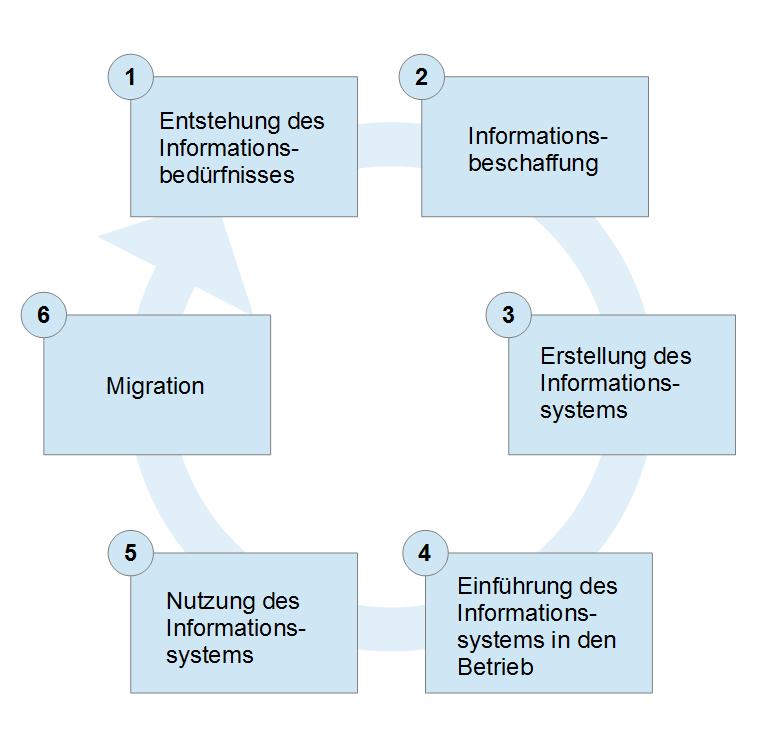
\includegraphics[width=10cm]{kapitel/gruppe1_1/bilder/informations-lebenszyklus}
	\caption{Informations-Lebenszyklus}
	\label{fig_informations_lebenszyklus}
\end{figure}

Ich bin ein Satz, der sich auf Abbildung \ref{fig_informations_lebenszyklus} bezieht und die Quelle dazu angibt.\footnote{Was ist meine Quelle?}
\todo[inline]{Ich bin ein Satz, der sich auf Abbildung \ref{fig_informations_lebenszyklus} bezieht und die Quelle dazu angibt.}

\subsection{Informationsmanagementmodell in der Literatur}
In der deutschsprachigen Literatur lassen sich viele verschiedene Arbeiten und Definitionen zum Thema Informationsmanagement finden, die sich zum Teil deutlich voneinander unterscheiden. Im Folgenden wollen wir kurz auf die Informationsmanagementmodelle- und Sichtweisen von Heinrichs, Wollnik und Krcmar eingehen.

\subsection{Informationsmanagement nach Heinrich}

Lange Zeit stellte das 1987 erschienene Werk von Lutz Heinrich das deutschsprachige Standardwerk im Bereich des Informationsmanagement dar.\footnote{\cite{heinrich_informationsmanagement_2005}} Entsprechend wurde es auch als Lehrbuch an Hochschulen eingesetzt.\footnote{\cite{heinrich_inm_2002}}

Laut Heinrich wird unter Informationsmanagement das “Leitungshandeln (Management) im Unternehmen im Bezug auf Information und Kommunikation” verstanden.\footnote{\cite{heinrich_informationsmanagement_2005}}

Es umfasst alle Führungsaufgaben, die sich mit Information und Kommunikation befassen. Diese Informations- und Kommunikationsaufgaben werden als Informationsfunktion bezeichnet, die den Schwerpunkt des Informationsmanagements darstellt. 

Das Ziel des Informationsmanagements laut Heinrich ist es, eine Informationsinfrastruktur aufzubauen, die die Verteilung, Produktion und Nutzung vom Informationen zur Aufgabe hat. Die Informationsinfrastruktur dient dazu, das Leistungspotenzial der Informationsfunktion umzusetzen und somit einen optimaler Beitrag zum Unternehmenserfolg zu leisten.\footnote{\cite{heinrich_inm_2002}}

Für die Umsetzung der Ziele werden die Aufgaben des Informationsmanagements in drei Ebenen strukturiert.
Die \textbf{strategische} Ebene plant, überwacht uns steuert die Informationsinfrastruktur.
Die \textbf{administrative} Ebene plant, überwacht und steuert die Komponenten der Informationsinfrastruktur (z.B. Anwendungssysteme, Mitarbeiter, Bestand an Daten).
Die \textbf{operative} Ebene umfasst Aufgaben und Nutzung der Informationsinfrastruktur. Mögliche Aktionsfelder für die operative Aufgabenebene stellen den laufenden Betrieb, die Nutzerunterstützung und die Störungsbeseitigung dar.

Auf jeder Aufgabenebene werden Methoden, Techniken und Werkzeuge eingesetzt, die die Durchführung 
der strategischen, administrativen und operativen Aufgaben durchführt und unterstützt.
Die Gesamtheit dieser Methoden und Techniken wird von Heinrich als \emph{Information Engineering} bezeichnet.

\subsection{Informationsmanagement nach Wollnik}
Michael Wollnik\footnote{\cite{wollnik_referenzmodell_1988}} gliedert das Informationsmanagement in drei Ebenen.

Die \textbf{Ebene des Informationseinsatzes} und dessen Management befasst sich mit der Integration von Informationen in Produkte und Dienstleistungen. Des weiteren befasst es sich mit der Erschließung neuer Märkte durch den Einsatz von Informationstechnologie.

Die \textbf{Ebene der Informations- und Kommunikationssysteme} stellt die mittlere Managementebene dar. Laut Wollnik bestehen Informationssysteme aus folgenden Elementen/Komponenten: Aufgaben, Informationen, Personen, Geräte, Organisation und Programme. Diese bestimmen die Struktur eines Informationssystems. Die Aufgaben dieser Ebene sind die Festlegung, Erhaltung und Modifikation dieser Strukturen während des Lebenszyklus des Informationssystems.

Ein weiteres Handlungsobjekt dieser Ebene sind die Prozesse zur Gestaltung von Informationssystemen, die geplant, organisiert und kontrolliert werden müssen. Diese Ebene stellt das Verbindungsglied zwischen den betrieblichen Aufgaben (Ebene Eins) und der technischen Infrastruktur (Ebene Drei) dar.

Die \textbf{Ebene der Informations- und Kommunikationsinfrastruktur} ist die unterste der drei Ebenen 
und befasst sich mit der Informationstechnologie. 
Dazu zählt laut Wollnik die Hard- und Software sowie die inhaltlichen Strukturen (zentrale Informationsbestände, Zugriffsberechtigungen auf Informationen). Kernaufgabe dieser Ebene ist der Betrieb und die Entwicklung der Infrastrukturen.\\

Diese drei Ebenen sind hierarchisch strukturiert und stellen den jeweils übergeordneten Ebenen Dienstleistungen zur Verfügung bzw. stellen Anforderungen an die jeweils untergeordneten Ebenen. 

\begin{figure}[h!]
	\centering
	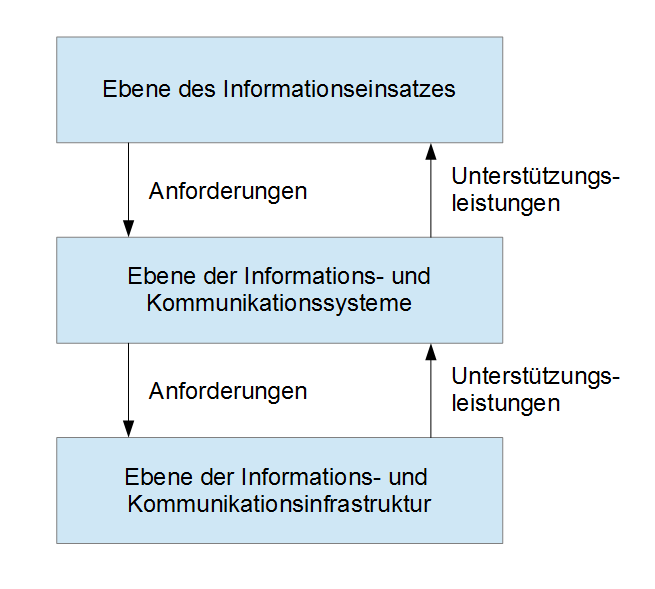
\includegraphics[width=10cm]{kapitel/gruppe1_1/bilder/ebenenmodell_wollnik}
	\caption{Ebenenmodell nach Wollnik}
	\label{fig_ebenenmodell_wollnik}
\end{figure}

Dieses einfache Ebenenmodell stellt auch die Grundlage für viele weitere Informationsmanagementmodelle dar, unter anderem das von Krcmar.

\subsection{Informationsmanagement nach Krcmar}
Krcmars Strukturierung des Informationsmanagement basiert auf dem Ebenenmodell von Wollnik, erweitert es jedoch um allgemeine Führungsaufgaben mit ebenenübergreifenden Funktionen (IT-Governance, Strategie, IT-Prozesse, IT-Personal, IT-Controlling).\footnote{\cite{krcmar_informationsmanagement_2015}}

Er gliedert das Informationsmanagement in die drei Teilbereiche Informationswirtschaft, Informationssysteme und Informations- und Kommunikationstechnik.

Die \textbf{Informationswirtschaft} beschäftigt sich mit dem Angebot, der Nachfrage und Verwendung von Informationen.
Die \textbf{Informationssysteme} haben das Management von Daten, Prozessen und dem Anwendungslebenszyklus zur Aufgabe.
Die \textbf{Informations- und Kommunikationstechnik} weisen die Speicherung, Verarbeitung und Kommunikation von Information als Basisfunktionalitäten auf.

In Kapitel \ref{section_inm_nach_krcmar} wird genauer auf den Aufbau des Informationsmanagementmodells von Krcmar eingegangen.

Da Krcmar mit seinen Publikationen zum Thema Informationsmanagement breiter aufgestellt ist als andere Autoren und er entsprechend oft zitiert wird, soll er auch in dieser Arbeit als Quelle für die nachfolgenden Kapitel sein. 

\subsection{Ziele des Informationsmanagements}
Das Informationsmanagement verfolgt zwei grundlegende Zielsetzungen.
Das erste Ziel ist die Koordination der Informationslogistik bzw. die Gewährleistung der adressatengerichteten Informationsversorgung.
Das zweite Ziel ist die Unterstützung der Unternehmensziele durch eine zielgerichtete und wirtschaftliche Steuerung der Informatik.\footnote{\cite{zarnekow_intergriertes_2004}}

Die Aufgaben des Informationsmanagements leiten sich aus diesen Zielen ab und werden im diesem Kapitel näher beleuchtet.

\subsection{Koordination der Informationslogistik}
In erster Linie ist das Ziel des Informationsmanagements, tatsächlich relevante Information von der Menge an verfügbaren und eventuell unnützen Informationen zu trennen, die für einen Entscheidungsprozess benötigt werden. Hierzu muss jedoch erst einmal ein Informationsbedarf vorliegen, der die Art, Menge und Beschaffenheit der Informationen bestimmt und auf dessen Grundlage eine Entscheidung getroffen werden kann.

Die Definition des Informationsbedarfs hängt einerseits vom Entscheider, andererseits von den Anforderungen der zu treffenden Entscheidung ab.

Der Informationsbedarf lässt sich grundsätzlich in zwei Kategorien einteilen: in den objektiven und den subjektiven Informationsbedarf.\footnote{\cite{picot_grenzenlos_2003}}

Der \textbf{objektive} Informationsbedarf wird in erster Linie durch die Entscheidung festgelegt und baut auf der Aufgabenbeschreibung des Entscheiders und den jeweiligen Marktgegebenheiten auf.
Der \textbf{subjektive} Informationsbedarf wird primär durch den Entscheider festgelegt. Welche Informationen für die Entscheidung relevant sind, werden durch die Einschätzungen und Präferenzen des Entscheiders mitbestimmt.

Aus der Überschneidung des objektiven und subjektiven Informationsbedarfs entsteht die Informationsnachfrage, die wiederum maßgeblich vom Informationsangebot abhängt. Somit legt der Informationsbedarf

\begin{itemize}
	\item die Beschaffenheit (Qualität),
	\item den Zeitpunkt der Lieferung,
	\item den Ort, an dem geliefert wird und
	\item das Medium, über das geliefert wird		 
\end{itemize}
in Bezug auf die Information fest. Im Hinblick auf die Unternehmensziele sollten die Informationen als Ressource angesehen werden.\footnote{\cite{bode_informationsbegriff_1997}} 

\subsection{Informationsmanagement als Unterstützung der Unternehmensziele}
Das Informationsmanagement bildet einen Teil der Unternehmensführung ab, der die Steuerung der Informatik (d.h. Mitarbeiter, Prozesse, organisatorische Teilbereiche und die eingesetzten Informationstechnologien) zur Verantwortung hat.

Die Rahmenbedingungen für die Informationslogistik werden so gestaltet, dass diese Informatik und deren Leistungen auf die Unternehmensziele ausgerichtet ist.\footnote{\cite{voss_informationsmanagement_2001}}

Dazu sollte eine geeignete und zweckorientierte Informationsinfrastruktur (Systemdenken, Rationalisierung, Orientierung am Beschaffungs- und Absatzmarkt) bereitgestellt werden.\footnote{\cite{Vgl. u.a. Vieweger, Bernd; Informationsmanagement; 2013}}
\todo[inline]{andere Quelle finden, da nicht mehr verfügbar}

\section{Aufbau des Informationsmanagements nach Krcmar - AD}
\textit{Alina Düßmann}


Prof. Dr. Helmut Krcmar, 1954 in Hanau geboren, schloss sein Studium der Wirtschaftswissenschaften an der Universität des Saarlandes ab und hat derzeit den Lehrstuhl der Wirtschaftsinformatik der Technischen Universität München inne.

Im Rahmen seines beruflichen Werdeganges widmete er sich der Forschung  auf dem Gebiet der Wirtschaftsinformatik, insbesondere dem Informationsmanagement.

Krcmars Ziel ist es, eine fokussierte und strukturierte Darstellung der Grundzüge des Informationsmanagements zu geben, mit dem Fokus auf der Präsentation ausgewählter Themen, Methoden und Konzepten.

Als Autor verschiedener veröffentlichter Werke hat Krcmar die Ansichtsweise des
Informationsmanagements in Deutschland revolutioniert. Aus seiner Hand stammen die
meisten Publikationen zum Thema Informationsmanagement aus informationstheoretischer
Perspektive.\footnote{\url{ttp://www.professoren.tum.de/krcmar-helmut/}, abgerufen am 09.05.2015, verfasst von Dr. Ulrich Marsch}

Das Informationsmanagement hat als primäre Aufgabe die betriebswirtschaftlich sinnvolle Steuerung von Informationen, die nach Krcmar als Ressource beschrieben werden.

Die Gestaltungsmöglichkeiten der innerbetrieblichen Informationswirtschaft im Spannungsfeld zwischen dem technologisch Realisierbarem, den arbeitsorganisatorischen Anforderungen der Mitarbeiter an Informationssysteme, der organisatorischen Konfiguration selbst und dem wettbewerblichen Umfeld der Organisation geben dem Informationsmanagement Bedeutung.\footnote{fortiss GmbH, Autor unbekannt, 2015, \url{http://www.fortiss.org/ueber-uns/mitarbeiter/helmut-krcmar/}, abgerufen am 09.05.2015}

Der Autor verfolgt das Ziel, eine fokussierte und strukturierte Darstellung der Grundzüge des Informationsmanagements zu geben. Das Informationsmanagement ist laut seiner Definition eine Managementaufgabe.

Drei Kernbereiche sind hier zu berücksichtigen.
\begin{enumerate}
	\item Das Management der Informationswirtschaft
	\item Das Management der Informationssysteme
	\item Das Management der Informations- und Kommunikationstechnik
\end{enumerate}

Das Informationsmanagement in die Organisations-, Führungs- und Kontrollstrukturen zu integrieren unterliegt dem Management der Unternehmensführung.

In seinen Werken definiert Krcmar einleitend die Grundbegriffe des Informationsmanagements.\\

\textbf{Information}\\\\
Das Wort „Information“ ergibt sich auf Grund einer Abbildung \ref{fig_ebenen_begriffshierarchie}, die den Zusammenhang zwischen Zeichen, Daten, Informationen und Wissen auf vier Ebenen darstellt.

\begin{figure}[h!]
	\centering
	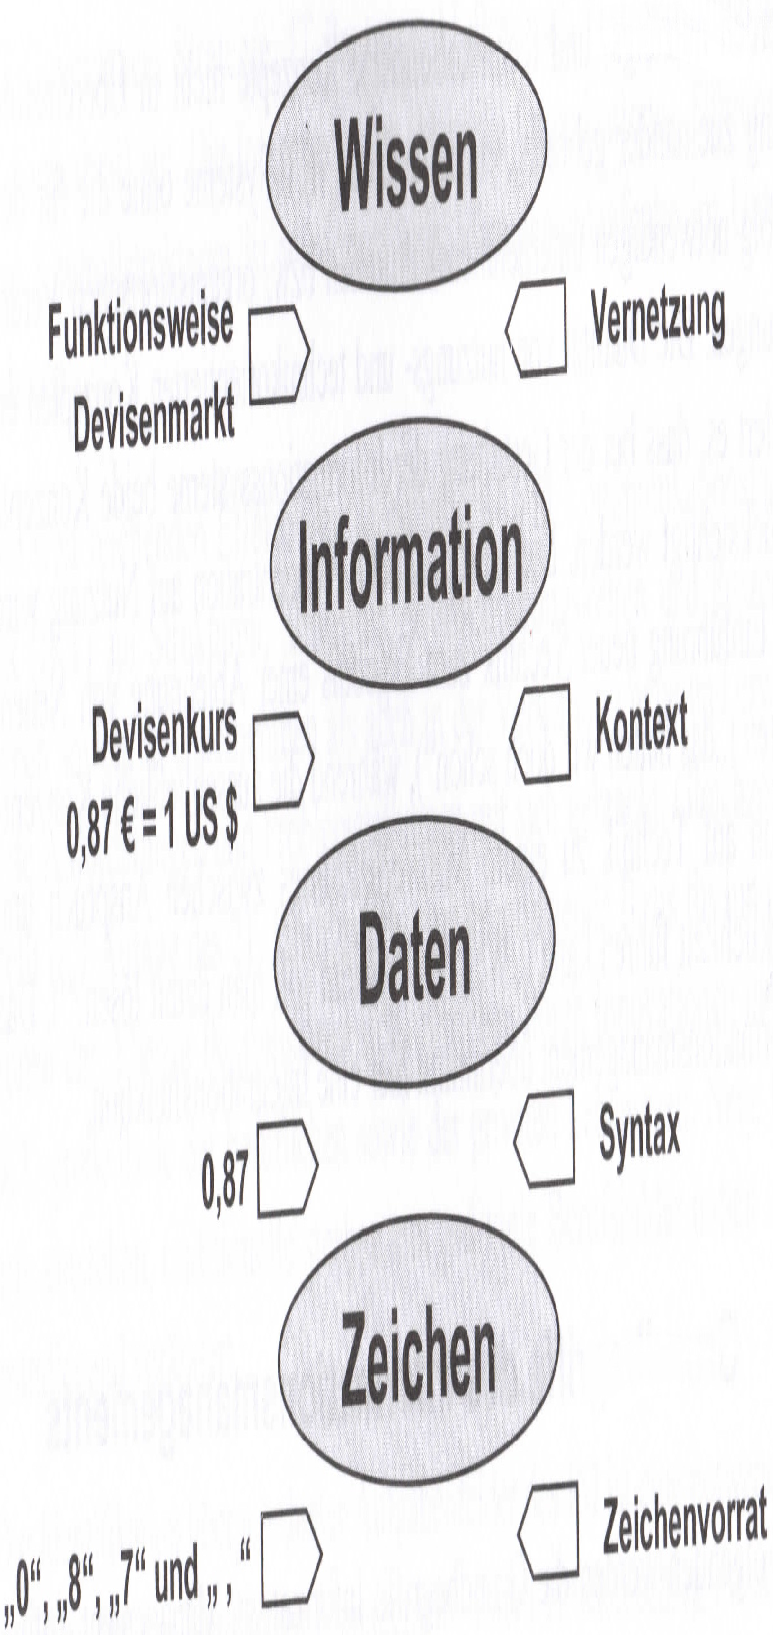
\includegraphics[width=10cm, height=8cm]
	{kapitel/gruppe1_1/bilder/ebenen_der_begriffshierarchie}
	\caption{Die Beziehungen zwischen den Ebenen der Begriffshierarchie, nach Krcmar}
	\label{fig_ebenen_begriffshierarchie}
\end{figure}

Wie in dieser Grafik von Krcmar\footnote{\cite{krcmar_einfuhrung_2015}} zu erkennen, befindet sich auf der untersten Ebene ein Zeichenvorrat als Basis aller weiteren oben angesiedelten Begriffe. 
Aus diesem Zeichenvorrat entstehen Daten, wenn die Zeichen in einen definierten, strukturierten Zusammenhang gebracht werden.
Werden diese entstandenen Daten mit Kontext angereichert, bekommen sie eine Bedeutung, sodass eine Information entsteht. 
Durch die Vernetzung dieser Information mit anderen Informationen entsteht Wissen auf einer übergeordneten Begriffshierarchie.

Wird Information als Produktionsfaktor im betrieblichen Leistungsprozess angesehen, 
versteht sie sich in diesem Zusammenhang als eine immaterielle, aber nicht kostenlose Ressource.

Des Weiteren bringen Informationen dem Verwender einen Nutzen, wenn sie in Handeln umgesetzt werden. Informationen sind keine keine freien Güter, weshalb sie keinen kostenadäquaten Wert haben können.

Der Wert hängt von der kontextspezifischen und zeitlichen Verwendung ab. Sie sind darüber hinaus auch erweiterbar und verdichtbar. Über die Qualität entscheiden mehrere Einflussfaktoren, wie beispielsweise die Vollständigkeit, die Genauigkeit und die Zuverlässigkeit.

Informationen werden kodiert übertragen, weshalb für ihren Austausch gemeinsame Standards notwendig sind.\\

\textbf{Management}\\\\
Im funktionalen Sinne beschreibt das Management spezielle Aufgaben und Prozesse, die unternehmensintern und zwischen Unternehmen stattfinden.
Diese Aufgaben werden wiederum unterteilt in Personalfunktionen und Fachfunktionen. In den Aufgabenbereich der Personalfunktionen fallen die persönliche Betreuung, sowie die soziale Integration der Mitarbeiter, im Sinne der Arbeitsplatzgestaltung und der Personalförderung.

Aus den Fachfunktionen lässt sich die Unterstützung an der Realisierung der Unternehmensziele ableiten. Planung (Zielvorgabe, Problemanalyse, Alternativensuche), Entscheidung sowie Realisierung und Kontrolle stehen im Mittelpunkt.
Dem Management als Institution gehören alle Personen an, die als Entscheidungsträger ständig personen- und sachbezogene Aufgaben wahrnehmen: Vorstand, Führungskräfte, Stäbe.\\

\textbf{Informationssysteme}\\\\
Bei Informationssystemen (IS) handelt es sich um soziotechnische („Mensch-Maschine-“) Systeme, die menschliche und maschinelle Komponenten (Teilsysteme) umfassen und zur Bereitstellung von Informationen und Kommunikation nach wirtschaftlichen Kriterien eingesetzt werden.

Planung und Bereitstellung der Informationssysteme des Unternehmens zur Erfüllung betrieblicher Aufgaben stellen damit einen Teilbereich der Informationsmanagement-Aufgaben dar.\\ 

\textbf{Informations- und Kommunikationstechnik}\\\\
Informations- und Kommunikationstechnik (IKT) ist die Gesamtheit der zur Speicherung, Verarbeitung und Kommunikation zur Verfügung stehenden Ressourcen, sowie die Art und Weise, wie diese Ressourcen organisiert sind.
Es stellt die Basis für ein erfolgreiches Informationsmanagement dar.
Die Basistechnik bezeichnet die Basiseinheiten der IKT zur Bereitstellung der Basisfunktionalitäten Verarbeitung, Speicherung und Kommunikation für die einzelnen zur Verfügung stehenden Ressourcen.
Für bestimmte Anwendungen sinnvolle Kombinationen von Basistechniken zur Realisierung spezieller Konzepte werden als Technikbündel beschrieben.\footnote{\cite{krcmar_einfuhrung_2015}}

Das Modell des Informationsmanagements basiert auf folgender Definition des Informationsmanagements:
„Informationsmanagement ist das Management der Informationswirtschaft, der Informationssysteme, der Informations- und Kommunikationstechnik sowie der übergreifenden Führungsaufgaben. Das Ziel des IM ist es, den im Hinblick auf die Unternehmensziele bestmöglichen Einsatz der Ressource Information zu gewährleisten. IM ist sowohl Management- als auch Technikdisziplin und gehört zu den elementaren Bestandteilen der Unternehmensführung.“\footnote{\cite{krcmar_einfuhrung_2015}}

\begin{figure}[h!]
	\centering
	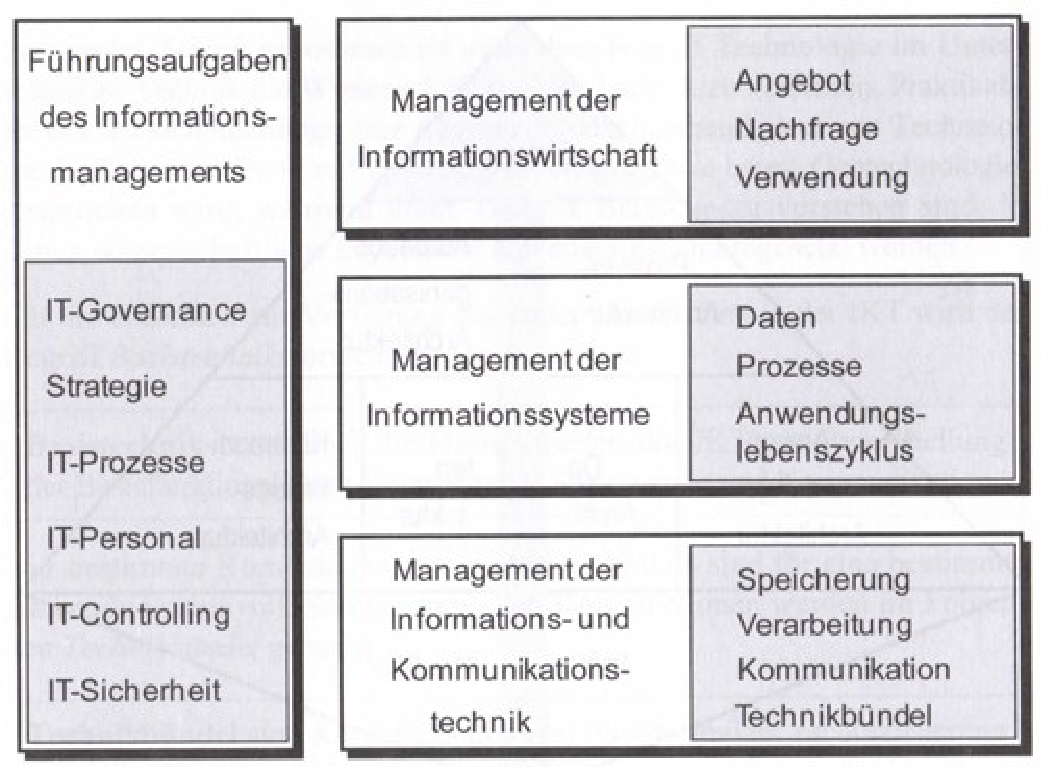
\includegraphics[width=10cm, height=8cm]
	{kapitel/gruppe1_1/bilder/modell_des_inm}
	\caption{Modell des Informationsmanagements, nach Krcmar}
	\label{fig_modell_des_inm}
\end{figure}

Das Informationsmanagement ist eine Managementaufgabe. Wie in Abbildung \ref{fig_modell_des_inm} zu sehen ist, besteht die Basis aus dem \textbf{Management der Informations- und Kommunikationstechnik}.

Auf dieser Ebene stehen die Speicherungstechnik, die Verarbeitungstechnik, die Kommunikationstechnik und die Technikbündel im Fokus.

Es wird die physische Basis für die Anwendungslandschaft auf der mittleren Ebene gelegt und damit die Bereitstellung der Informationsressourcen.

Auf der mittleren Ebene, der des Managements der Informationssysteme, liegen die Kernaufgaben im Management der Daten, der Prozesse und des Anwendungslebenszyklus. Die Ebene wird von der IKT unterstützt. Das Management der Anwendungsentwicklung erfolgt beispielsweise auf dieser Ebene.

Auf der Ebene des Managements der Informationswirtschaft besteht das Handlungsobjekt aus der Ressource Information. Es geht um den Informationseinsatz zur Deckung des Informationsbedarfs. Dieses Informationsangebot wird im Rahmen eines informationswirtschaftlichen Planungszyklus geplant, organisiert und kontrolliert.

Die Ebenen bauen also aufeinander auf. Als Ergebnis des Ordnungsrahmens können nun die einzelnen Aufgaben des Informationsmanagements identifiziert und zugeordnet werden. Die Differenzierung in drei Ebenen und einem übergreifenden Aufgabenblock zeigt, dass die Aufgaben des Informationsmanagements verteilt durchgeführt werden. Die Verteilung dieser Aufgaben gehört zur Führungsaufgabe „IT-Governance“.

Die Herstellung des informationswirtschaftlichen Gleichgewichts zwischen Informationsangebot und Informationsnachfrage bildet das Ziel des Managements der Informationswirtschaft. Das Gleichgewicht ist dynamisch, was bedeutet, dass Angebot und Nachfrage immer wieder aufeinander eingestellt werden müssen. Somit muss auch der Managementprozess der Informationswirtschaft regelmäßig ein neues Gleichgewicht suchen, sobald sich ein Parameter ändert.

Daraus ergibt sich der Lebenszyklus der Informationswirtschaft. Er besteht aus 5 Elementen aus Aktivitäten:
\begin{itemize}
	\item Management der Informationsnachfrage
	\item Management der Informationsquellen
	\item Management der Informationsressourcen
	\item Management des Informationsangebots
	\item Management der Informationsverwendung
\end{itemize}

\begin{figure}[h!]
	\centering
	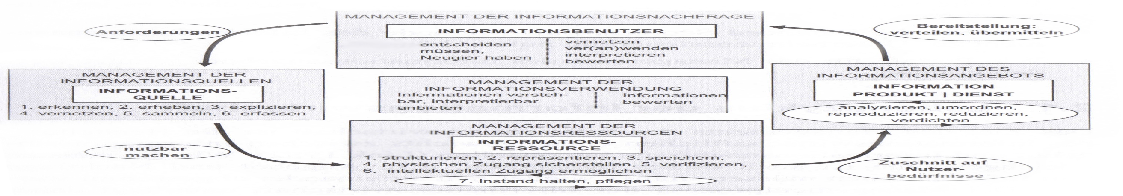
\includegraphics[width=\textwidth, height=10cm]
	{kapitel/gruppe1_1/bilder/lebenszyklus_der_informationswirtschaft}
	\caption{Lebenszyklusmodell der Informationswirtschaft, nach Krcmar}
	\label{fig_lebenszyklus_informationswirtschaft}
\end{figure}

In Abbildung \ref{fig_lebenszyklus_informationswirtschaft} lassen sich die fünf Elemente des Zyklus erkennen. Das Management der Quellen, Ressourcen, des Angebotes und der Nachfrage agieren als Teilmanagementaufgaben um das Management der Informationsressourcen.

Stehen Informationen einem Informationsbenutzer zur Verfügung, die durch einen informationswirtschaftlichen Zyklus erschlossen wurden, kann der Informationsbedarf gedeckt werden.

Der Informationsbenutzer interpretiert die von ihm gewünschten Informationen entsprechend dem verfolgten Zweck und bringt sie zur Anwendung.
Dabei entstehen neue Informationen, da der Informationsbenutzer die angebotenen Informationen interpretiert, bewertet und mit seinen bereits vorhandenen Informationsstrukturen kombinieren kann.
Ergebnis dieser Bewertung ist, dass der Informationsbedarf gedeckt wurde oder nicht. Dementsprechend muss das Informationsangebot ausgeweitet oder verändert werden.\footnote{\cite{krcmar_einfuhrung_2015}}\\

\textbf{Software-Einführung}\\\\
Eine Möglichkeit für die Einführung von Software ist es, auf Standardsoftware zurück zu greifen. Andererseits können Unternehmen die Software auch selbst entwickeln, wobei Softwareentwicklungsmodelle behilflich sein können.

Der Anwendungslebenszyklus ist mit der Auswahl und Anpassung von Software noch nicht abgeschlossen., sondern erreicht die operative Nutzung erst nach erfolgreicher Einführung.

Die Einführung von Software umfasst nicht nur die Installation, sondern auch die Schulung des Personals und die Inbetriebnahme.

Zudem wird noch zwischen folgenden Konzeptionen unterschieden: 
\begin{itemize}
	\item die Stichtagsumstellung
	\item die Parallelisierung
	\item die Teilweise Einführung und
	\item die Versionsumstellung
\end{itemize}
\newpage
\textbf{Technochange}\\\\
Die Einführung von Software – im Allgemeinen von Informations- und Kommunikationstechnik-Systemen (IKT-Systemen) – kann bedeutende Veränderungen in der Arbeitsweise von Mitarbeitern auslösen. 

Diesem Prozess liegt ein hohes Leistungssteigerungspotential zugrunde, allerdings ein ebenso großes Risikopotential. 

So kann z.B. ein neu eingeführtes IKT-System von den Mitarbeitern abgelehnt werden. Diese Veränderung wird als Technochange bezeichnet, welcher 4 Phasen durchläuft. In Abbildung \ref{fig_technochange_lebenszyklus} sind diese Phasen zu sehen.
\begin{figure}
	\centering
	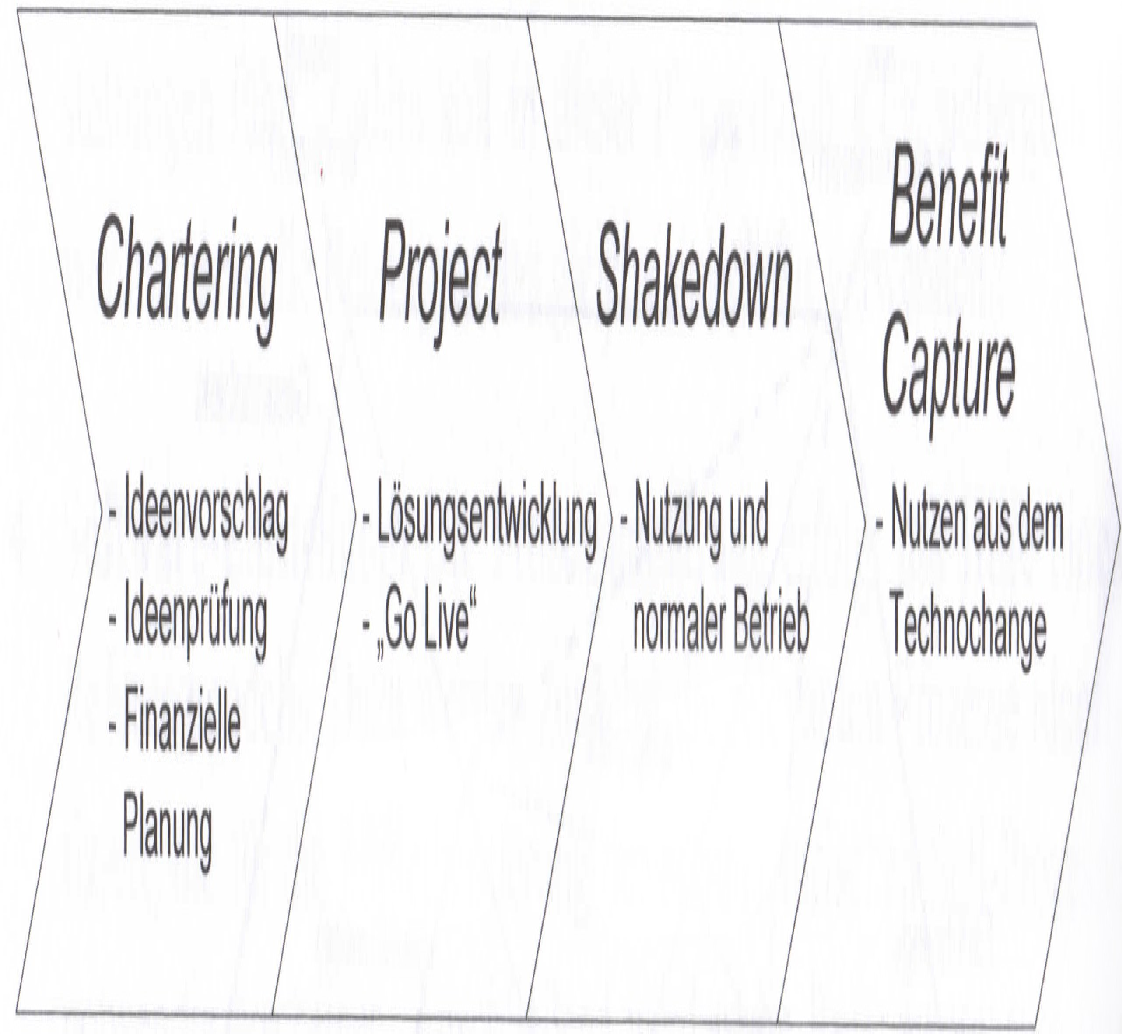
\includegraphics[width=10cm, height=4cm]{kapitel/gruppe1_1/bilder/technochange_lebenszyklus}
	\caption{Technochange-Lebenszyklus, nach Krcmar}
	\label{fig_technochange_lebenszyklus}
\end{figure}
Der Lebenszyklus ist eigentlich eher ein Lebenslauf, in dem die einzelnen Phasen – Chartering, Project, Shakedown und Benefit Capture – aufeinander aufbauen.\\

\textbf{Softwareentwicklungsmodelle}\\\\
Gut geplante Einzelschritte des Projekts und die Einkalkulation ggf. entstehende Probleme und deren Lösungsfindung entscheiden wesentlich über den Erfolg einer Anwendungsentwicklung.
Aufgrund der Dynamik innerhalb des Entwicklungsprozesses, muss die Projektplanung laufend aktualisiert werden.

Meilensteine, Ergebnisse, Ziele und Kriterien werden vor Beginn der Projektphase festgelegt. Verschiedene Optionen zur Projektdurchführung sind anhand der Kriterien zu bewerten und gegenüber zu stellen, und zwar sowohl vor Projektbeginn, als auch im Laufe des Projekts.

Im weiteren Verlauf durchläuft das Projekt einen Software-Zyklus mit mehreren Stadien.  Iterative Modelle haben sich in der Praxis durchgesetzt, mit fest definierten Phasen, die sequenziell durchlaufen werden.

Das Wasserfallmodell wurde durch die Integration qualitätssichernder Maßnahmen 1992 zum V-Modell weiterentwickelt und 1997 überarbeitet. Die Strukturierung anhand des V-Modells erfolgt anhand drei Ebenen:

Vorgehensweise (Was ist zu tun?)\\
Methode (Wie ist es zu tun?)\\
Werkzeuganforderungen(Womit ist etwas zu tun?)

Um die meist sehr komplexe Aufgabe erfolgreich umzusetzen, muss eine geeignete Projektorganisation aufgebaut werden.

Da die Einführung von Software eine besondere Herausforderung für Unternehmen mit sich bringt, sind Vorgehensmodelle von außerordentlicher Bedeutung. 
Diese haben das Ziel, den Ablauf einer Softwareentwicklung zu beschreiben und den Prozess zur Softwareentwicklung in handhabbare Teilaufgaben zu strukturieren. 
Dabei kann zwischen stark und weniger stark formalisierten sowie sequenziellen oder initiativen Vorgehensmodellen stark unterschieden werden. 
Die bedeutendsten Vorgehensmodelle sind das V-Modell, das Spiralmodell sowie der Rational Unified Process (RUP).

Ferner ist es notwendig die Einführung von Software wirtschaftlich zu rechtfertigen. Anhand von Verfahren zur Kostenschätzung können die Kosten für Entwicklung, Erwerb und Nutzung von Informationssystemen geschätzt werden und dadurch deren Wirtschaftlichkeit gerechtfertigt werden.\footnote{\cite{krcmar_einfuhrung_2015}}

Auch an Hochschulen ist es von großer Wichtigkeit das Gleichgewicht von Informationsangebot und -nachfrage in Balance halten zu können. 
Das hier ebenfalls dynamische Gleichgewicht ist an den Informationsbedarf der Hochschulangehörigen angelehnt. 
Dieser Personenkreis umfasst nicht nur die Studenten, sondern auch die Hochschulangestellten. 
Es ist Aufgabe des Hochschulpersonals die Informationsnachfrage der Studierenden und Studienbewerber mit einem Informationsangebot zu decken, welches bezüglich der Qualität der Informationen eine Bedarfsdeckung verspricht. 
Die Entscheidung, ob Standardsoftware verwendet werden soll, oder ob sie hochschulintern entwickelt werden soll, ist unter den Hochschulen individuell getroffen. 
Es gilt gewisse Faktoren zu beachten, die in den Entscheidungsprozess Einfluss nehmen, wie beispielsweise der zeitliche Aufwand der Entwicklung, Testphasen oder die Kosten. 
Die bereits genannten Softwareentwicklungsmodelle tragen zur Entscheidungshilfe bei.
Die Einführung einer Software kann einen Technochange beinhalten und birgt dadurch große Risiken. 
Der Mensch ist nur ungern von seinen Gewohnheiten abzubringen, wodurch auch die Umstellung hochschulinterner Systeme Frustration und Unmut auslösen kann, was den Arbeitsaufwand der Studentenbetreuung erhöht.

\subsection{Management der Schnittstellen zu den Informationsempfängern}
Die Schnittstelle beschreibt in diesem Zusammenhang den „Berührungspunkt“ in dem die Informationen ausgetauscht werden. 
Die beteiligten Individuen sind in diesem Fall Personen, die über technische Kommunikationsmittel Informationen erhalten oder senden. 
Beispielsweise bekommen Studenten Informationen von ihrem Tutor, über Tag und Uhrzeit des nächsten stattfindenden Tutoriums. 

Es handelt sich hier um eine zweiseitige Mensch-Computer-Interaktion (Smartphone, Tablet, Laptop hier synonym verwendet), da die Individuen über eine Benutzerschnittstelle ihres Computers jeweils miteinander über technische Hilfsmittel Informationen austauschen.
Damit eine Benutzerschnittstelle für den Menschen nutzbar und sinnvoll ist, muss sie auf seine Bedürfnisse und Fähigkeiten angepasst sein. 
Eine gewisse Grundlagenkenntnis im technischen Umgang, sowie mit Social-Media- oder Forennutzung, wird in diesem Fall, im Rahmen der Digital-Natives-Generation, vorausgesetzt.\footnote{\url{http://de.wikipedia.org/wiki/Digital_Native}, abgerufen am 13.05.2015}

Somit ist die Voraussetzung des verständlichen Umgangs mit Informationsmedien erfüllt, sodass im nächsten Schritt dafür gesorgt werden muss, dass Informationen vorhanden sind, die übermittelt werden können. 
Beispielhaft wäre es hier anzunehmen, dass ein Informatikstudent, durch die Zugehörigkeit in seinem Fachbereich und seinem entsprechenden Studiengang durch Hochschulpersonal fachbereichsbezogene Informationen durch den Zugang zum Informationsportal der Hochschule erhält. 
Dies kann durch einen E-Mailverteiler oder eventuell durch ein Informationssystem mit entsprechenden Zugangsvoraussetzungen (wie Immatrikulation) gewährleistet werden. 
Das verwendete Informationsmedium stellt hier die Schnittstelle zwischen Mensch und der Ressource Information dar und bietet die Möglichkeit für den Studenten, gewünschte Informationen, die ihn betreffen, zu erhalten.

Auch hier ist das Qualitätsmanagement der zu verwaltenden Informationen ein essentielles Thema. 
Im Beispiel des Informatikstudenten sind für ihn die Informationen interessant, die ihn betreffen. 
Die Informationen zum Studiengang „Hispanistik“ sind für ihn irrelevant. 
Somit müssen Informationen, im Rahmen der Schnittstellenbetreuung, für die Empfänger vorselektiert werden, um keine Informationsüberflutung zu provozieren oder zu vermeiden, dass die übermittelte Information den Informationsbedarf nicht vollständig deckt und dadurch Rückfragen offen bleiben. 
Es ist also darauf zu achten, dass eine Information nicht vorzeitig veröffentlicht wird, ohne dass der Inhalt geprüft wurde. 
Als Beispiel könnte hier die Information „Der Kurs findet heute nicht statt.“ betrachtet werden, die für den Studenten zwar eine Teilinformation enthält, den Informationsbedarf aber nicht abdeckt, sodass eine Rückfrage entsteht, die zusätzlich verwaltet werden muss. 
Hochschulindividuell kann es auch automatisierte Informationssysteme geben, die von mehreren Plattformen zugreifbar sind, wobei auch hinter dieser Automatisierung Personal steht, das die entsprechende Information generiert. 
Auf das Qualitätsmanagement wird im folgenden noch detaillierter eingegangen.

Ein weiterer wichtiger Punkt ist, dass die Möglichkeit des Feedbacks seitens des Informationsempfängers gewährleistet sein muss. 
Ob dies nun in Form von Kontaktformularen oder über eine, zur Verfügung gestellte, E-Mail-Adresse geschieht, ist hochschulintern individuell. 
Von großer Bedeutung ist dieser Punkt, weil es beispielsweise im Falle einer nicht bedarfsdeckenden Information zu Verwirrungen und Missverständnissen kommen kann. 
Die Informationsempfänger brauchen also die Möglichkeit zur Rücksprache, um die Motivation nicht zu beeinträchtigen und ggf. Stresssituationen zu umgehen. 
Das Spektrum der Feedbackmöglichkeit ist mit der Möglichkeit der direkten Rücksprache noch nicht ausgeschöpft. 
Es gibt viele Möglichkeiten Feedback zu geben bzw. zu erhalten, wie beispielsweise eine Evaluationsdurchführung o.ä..
\section{Qualitätsmanagement der Informationsprozesse - MB}
\textit{Autor: Miriam Börger}


Im Folgenden wird der Qualitätsmanagement-Prozess in seinen Grundzügen definiert, am konkreten Beispiel der Minimierung von Durchlaufzeiten genauer betrachtet und praktisch mit Hilfe der IT Balanced Scorecard durchexerziert. 
Abschließend wird erörtert, welche Besonderheiten hierbei an Hochschulen bestehen und Möglichkeiten aufgezeigt, diese Schwierigkeiten zu umgehen.

\subsection{Aufgaben des Qualitätsmanagements}
In einem Informationsmanagement bildet das Qualitätsmanagement der Informationsprozesse einen zentralen Aufgabenbereich. Es übernimmt die Planung, Koordination und Steuerung der Informationsflüsse und prüft fortwährend, inwieweit eine Nutzbarkeit und Effizienz der Prozesse in der Realität gewährleistet ist, um deren Qualität gegebenenfalls mit gezielten Maßnahmen zu optimieren.\footnote{\cite{schroder_wertorientiertes_2005}}

Hierzu fungiert ein Team von Qualitätsmanagern als Vermittler zwischen den verschiedenen Parteien im Unternehmen und überbrückt potentiell auftretende Kommunikations- oder Kulturbarrieren, um eine zielorientierte und effiziente Informationsversorgung der beteiligten Parteien zu ermöglichen.

Zu Beginn des Qualitätsmanagement-Prozesses gilt es, eine Leitstrategie aufzustellen. Hierfür wird der aktuelle Ist-Zustand des Unternehmens in Bezug auf seine Organisation von Informationsflüssen analysiert. Dabei zum Vorschein kommende Schwachstellen werden erfasst und durch mögliche optimierende Handlungsoptionen ergänzt.\footnote{\cite{helmke_management_2013}}

Während der Durchführung der neu erschaffenen Maßnahmen ist das Qualitätsmanagement-Team mit der stetigen Überwachung dieser betraut. 
Bereits bei kleinen Abweichungen vom Plan kann mit gegensteuernden Maßnahmen eingegriffen werden. 
Eine im Voraus aufgestellte Zeitplanung ist hierbei ebenso wichtig wie eine klare Definition der Zuständigkeiten im Qualitätsmanagement-Team, um eine termingerechte Erreichung der gesetzten Ziele noch zu garantieren.

Nach Ablauf des gesetzten Zeitrahmens oder nach Beendigung der Maßnahmen ist es erforderlich, mittels einer sogenannten Feedback-Analyse festzustellen, inwieweit das gesteckte Ziel erreicht wurde und aus welchen Gründen es nicht zu 100\% zufriedenstellenden Ergebnissen kommen konnte. 
Die hieraus resultierenden Erkenntnisse bilden daraufhin die Grundlage für eine anschließende Feedforward-Analyse, die die weitergehend erforderlichen Maßnahmen feststeckt, um in einer weiteren Phase die Zielerreichung durch verbesserte Maßnahmen zu garantieren.\footnote{\cite{gadatsch_it-controlling_2012}}

\subsection{Prozessoptimierung durch Minimierung der Durchlaufzeiten}
Essenzielles Ziel des Qualitätsmanagement-Teams ist es, anhand bewährter Vorgehensweisen die Durchlaufzeiten von Informationen zu minimieren. 
Hierdurch wird der Informationsfluss quantitativ und qualitativ verbessert, da bestehende Abhängigkeiten der Parteien in Bezug auf die Informationen schneller bedient werden können und somit durch minimierte Wartezeiten eine beträchtliche Budgetersparnis resultiert.

\begin{figure}[h!]
	\centering
	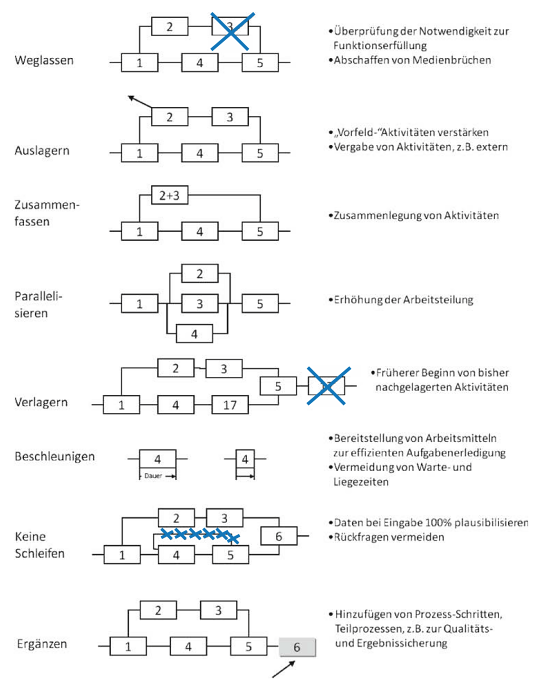
\includegraphics[width=10cm]{kapitel/gruppe1_1/bilder/minimierung_durchlaufzeiten}
	\caption{Minimierung von Durchlaufzeiten, nach Bleicher 1991, 196}
	\label{fig_minimierung_durchlaufzeiten}
\end{figure}

Wie in Abbildung \ref{fig_minimierung_durchlaufzeiten} erkennbar, existieren elementare Methoden zur Reduktion von Durchlaufzeiten nach Bleicher aus dem Jahre 1991, die noch heute ihre Gültigkeit in der Anwendung haben.\footnote{\cite{bleicher_organisation_1991}}

Insbesondere das Zusammenfassen von Aktivitäten hat den entscheidenden Vorteil, dass Abstimmungsprozesse und Abhängigkeiten zwischen mehreren Parteien entfallen und somit die Umsetzungsdauer auf ein Minimum reduziert wird. 

Auch die Methode des Parallelisierens sollte in den Fokus gerückt werden. Wie in Abbildung 1 ersichtlich, werden hierbei mehrere Parteien, die für eine darauffolgende Partei relevant sind, zeitgleich geschaltet, um Wartezeiten zu verhindern. 

Zu guter Letzt sei das Ergänzen von Prozessschritten betont. Auf den ersten Blick scheint diese Methode paradox, da durch Ergänzung weiterer Parteien der Zeit- und Arbeitsaufwand vorerst erhöht wird. Durch einen globaleren Blick wird schnell deutlich, dass ohne diese Parteien zu einem späteren Zeitpunkt Problematiken entstehen können, die in ihrer Lösung viel zeit- und arbeitsintensiver sind und das Unternehmen in seiner Prozessqualität deutlich zurückwerfen könnte.

Die in Abbildung \ref{fig_minimierung_durchlaufzeiten} gezeigten Methoden zur Durchlaufzeit-Minimierung sollten also vom Qualitätsmanagement-Team von Beginn an in die Planung mit einbezogen werden, da mit minimalem Aufwand eine weitreichende, inhaltlich und finanziell positive Auswirkung auf die Qualität des Gesamtprozesses erzeugt wird. 

\subsection{Anwendung des Qualitätsmanagements am Beispiel der IT Balanced Scorecard}
Das strategisch-operative Konzept für eine qualitative Unternehmenssteuerung aus den 90er Jahren von R. S. Kaplan und D. P. Norton hat sich im Laufe der Zeit zum Standardinstrument entwickelt.\footnote{\cite{friedag_scorecard_2004}}

Grundlegend für die IT Balanced Scorecard ist das Schema Eingabe $\to$ Verarbeitung $\to$ Ausgabe $\to$ Resultat. Die Kombination von Qualität der Mitarbeiter, Kundenorientierung und finanzielle Ziele ermöglicht die Generierung und Sicherung eines gelungenen Informationsmanagements.\footnote{\cite{gabriel_inm_2003}}

\begin{figure}[h!]
	\centering
	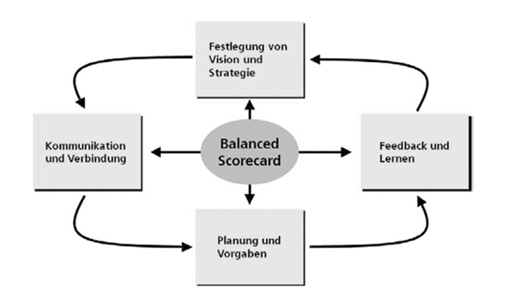
\includegraphics[width=10cm]{kapitel/gruppe1_1/bilder/balanced_scorecard}
	\caption{Balanced Scorecard Kreislauf, nach Gadatsch}
	\label{fig_balanced_scorecard_cycle}
\end{figure}

Die IT Balanced Scorecard zeichnet sich – wie in Abbildung \ref{fig_balanced_scorecard_cycle} deutlich wird – durch eine stetige Feedback- und Feedforward-Kommunikation aus. 
Zu Beginn des Managementprozesses werden in der Phase „Planung und Vorgaben“ die grundlegenden Ziele des Unternehmens definiert.

In einem nächsten Schritt werden in der Phase „Vision und Strategie“ Kernaussagen zur Strategiefindung erarbeitet, insbesondere im Hinblick auf den Zusammenhang von Ursache und Wirkung, sowie Optimierungsmöglichkeiten zusammengestellt. 

Das Handlungskonzept wird in „Feedback und Lernen“ final ausformuliert und in der vierten Phase „Kommunikation und Verbindung“ mit der Strategie und übergeordneten Zielen verknüpft.

Eine detaillierte Dokumentation von Teilzielen erhöht in dieser Phase die Motivation der Mitarbeiter zur Zielerreichung.\footnote{\cite{kaufmann_feinschliff_2002}}

Die Definition von klaren Zielen, Bedingungen und Kennzahlen generiert ein komplexes Kennzahlensystem, welches durch Herunterbrechen der Strategie auf operatives Handeln einen ganzheitlichen Überblick über die interne Organisation des Unternehmens liefert.

Die Einbeziehung von Ursache und Wirkung vereinfacht die vorausschauende Unternehmensführung und ergänzt die Sichtweise auf das Unternehmen zu einem ausgewogenen (balanced) Bild.

Da die Möglichekeiten zur Befüllung der Scorecard sehr vielseitig sind, sollte vermieden werden, sie mit zu vielen komplexen Zahlen zu überladen. 

Im Fokus stehen bei diesem Konzept vorrangig die Maßnahmenfindung unter Berücksichtigung von Ursache und Wirkung, was durch eine einseitige Betrachtung der Kennzahlen zu sehr in den Hintergrund rücken und den Lösungsprozess negativ belasten könnte.

\subsection{Besonderheiten an Hochschulen}
Ein gut funktionierendes Qualitätsmanagement kann nur effektiv und reibungslos funktionieren, wenn es an zentraler Stelle nahe des Entscheidungsträgers positioniert und gelebt wird.

Die Umsetzungsverantwortung eines ganzheitlichen Qualitätsmanagements liegt bei Hochschulen in der Regel bei der Hochschulleitung, die ihre Aufgaben im Prozess der Informationsflussoptimierung begreifen und verantworten muss.

Eine der grundlegenden Besonderheiten an Hochschulen liegt in der internen Strukturierung von Verantwortlichkeiten. Die Hochschule ist unterteilt in Fachbereiche, welche geschlossen für sich arbeiten können, aber dennoch der Hochschulleitung unterstellt sind. Zusätzlich zu diesen beiden Bereichen ist noch das Präsidium zu nennen, welches insgesamt für eine effiziente Aufgabenerfüllung und Interessenvertretung der Hochschule verantwortlich ist.\footnote{\cite{mintzberg_1992}}

Im Zuge der Einführung eines geordneten Qualitätsmanagements gilt es also, die Positionierung nahe der Hochschulleitung 
mit einer anwendungsbezogenen Platzierung innerhalb jedes Fachbereiches unter Einbeziehung des Präsidiums zu verknüpfen, 
um ganzheitliche Lösungen zur Realisierung eines Qualitätsmanagements zu finden und umsetzen zu können.

Ein Außenvorlassen des Fachbereichs, in dem die Lösungen schließlich umgesetzt werden, ist faktisch unmöglich. Durch die 
Vielzahl an Entscheidungsträgern und Mitredern besteht an Hochschulen ein höherer Bedarf an Kommunkations- und 
Abstimmungsleistungen zwischen diesen als in anderen Institutionen und Unternehmen. 

Es besteht zudem die Gefahr, dass Zuständigkeiten der verschiedenen Rollen an der entsprechenden Hochschule nicht klar 
geregelt sind, was die Funktionsweise des Entscheidungsprozesses zwar bestenfalls nicht beeinträchtigt, dessen Ablauf allerdings 
sehr unsystematisch gestaltet und den Fluss des Prozesses ausbremst.

Neben der strukturellen Schwierigkeiten in der Aufstellung eines Qualitätsmanagements besteht eine weitere Besonderheit in der inhaltlichen Vereinheitlichung der Anforderungen der einzelnen Parteien, die im schlechtesten Fall sehr verschieden sind oder sich gar widersprechen, sodass diese für alle Bereiche zentral gültig ist. 

Mithilfe renommierter Werkzeuge, wie z.B. der IT Balanced Scorecard, liegt es nun in der Hand des Qualitätsmanagement-Teams, 
die erarbeiteten Prozessstrategien und Maßnamen transparent für jeden Bereich der Hochschule einsehbar zu publizieren und 
alle betreffenden Personen über Änderungen zu informieren. 

Die Kontrolle in den Fachbereichen, ob und inwieweit die 
Maßnahmen zur Prozessoptimierung beitragen, darf hierbei nicht vernachlässigt werden.\footnote{\url{https://www.evalag.de/dedievl/projekt01/media/pdf/qm/audit/evalag_eckpunkte_qualitaetsmanagement.pdf}}


\section{Anwendung des Informationsmanagements am Beispiel von Hochschulen - MB}
\textit{Autor: Miriam Börger}

Mit der praktischen Anwendung der bisher erörterten Erkenntnisse zum Thema Informationsmanagement an Hochschulen befasst sich das nachfolgende Kapitel. 

Hierbei wird insbesondere analysiert, inwieweit der Bereich des Immatrikulations- und Prüfungsamtes als zentraler Knotenpunkt in der Informationsverteilung dienen kann und welche Auswirkungen sich für die Bibliothek und die Organisation von Rechnerpools ergeben können.

\subsection{Immatrikulations- und Prüfungsamt}
In Hochschulen, bei denen ein Informationsmanagement Anwendung findet, bildet das Immatrikulations- und Prüfungsamt eine Art interne Informationszentrale, welche weitere Bereiche mit notwendigen Informationen versorgt. 

Betrachtet an einem Beispiel bedeutet dies Folgendes: Bei Immatrikulation eines neuen Studierenden wird diesem vom Immatrikulationsamt eine Matrikelnummer zugewiesen und seine Stammdaten ins HIS eingepflegt. 

Nun ist es Aufgabe des Immatrikulationsamtes, das HIS zu einer Art Schnittstelle für alle wichtigen Hochschulbereiche, wie z.B. die Bibliothek, die Mensa oder auch die Verwaltung von Computerräumen, zu machen, sodass diese Bereiche via Eingabe der Matrikelnummer auf für sie wichtige Studierendendaten zugreifen können.

Um den Datenschutz der Studierenden zu garantieren, wäre hierfür eine Lösung mittels individueller Rechtezuweisung für jeden Bereich denkbar.

Der absolut saubere und stets aktuelle Datensatz im HIS wäre nicht nur zentral für alle Hochschulbereiche verfügbar, sondern auch jederzeit auf aktuellstem Stand, sodass Redundanzen ausgeschlossen werden können.

Zur Minimierung des Verwaltungsaufwandes wäre es denkbar, bei Stammdatenänderung durch das Immatrikulationsamt eine automatisch generierte E-Mail an alle beteiligten Bereiche mit den aktualisierten Informationen über den Studierenden zu versenden, was einem ganzheitlichen Informationsmanagement entsprechen würde.

Auch nach außen hin stellt das HIS eine zentrale Anlaufstelle für alle wichtigen Informationen wie Raumpläne, Kontaktdaten der Lehrenden und Prüfungsmodalitäten dar. 

Bei Ausfall einer Veranstaltung kann dieses dort direkt publik gemacht werden. Nach der Prüfungsanmeldung im HIS kann schnell und komfortabel aus den Anmeldedaten der Studierenden ein zentraler Raumbelegungsplan erzeugt werden.\footnote{\url{https://www.evalag.de/dedievl/projekt01/media/pdf/qm/audit/evalag_eckpunkte_qualitaetsmanagement.pdf}}

Bei der Notenvergabe meldet der Prüfer die Noten der Studierenden an das Prüfungsamt, welche diese in das HIS einpflegen. 
Die Studierenden haben nun die Möglichkeit zentral ihre Noten abzurufen. Auch die Fachbereiche, welche über die Leistungen ihrer Studierenden informiert werden sollten, können auf diese Daten zugreifen. 

Die Sammlung und Bereitstellung an zentraler Stelle wie dem HIS minimiert Abstimmungsmodalitäten zwischen den verschiedenen Hochschulbereichen, reduziert den Arbeitsaufwand für die erneute Erfassung und Verwaltung der Studierendendaten in dem jeweiligen Bereich und garantiert einen stets konsistenten Datensatz.

\subsection{Bibliotheken}
Hochschulbibliotheken werden tagtäglich mit einer Menge an Informationen und Daten konfrontiert. 
Von deren Besitz eines EDV-Systems zur Erfassung der Ausleihe inkl. Ablauf der Fristen und Stammdaten des Studierenden kann an dieser Stelle ausgegangen werden, da die Grundfunktionalität des Bibliothekssystems ansonsten kaum gewährleistet wäre.

Als weitere Basisfunktion sei die Autorisierung der Studierenden zu nennen. Bei der Ausleihe wird in Hochschulbibliotheken über das System geprüft, ob dieser Studierende durch Immatrikulation dazu berechtigt ist, an dieser Hochschule Bücher auszuleihen.

Im Zuge eines angewandten Informationsmanagements wäre es von Vorteil, die Stammdaten der Studierenden direkt aus dem HIS auszulesen. 

Aufbauend auf dieses Grundsystem existieren Lösungen, die das Bibliothekswesen mittels Informationsvermittlung, -speicherung und -auswertung für zahlreiche Einsatzmöglichkeiten bereichert.
 
Jede Hochschule sollte sich etwas Zeit nehmen, sich mit einer EDV-Lösung zu befassen, die neben der elektronischen Erschließung der Ausleihfaktoren auch Werkzeuge zur statistischen Erfassung, Messung und Bewertung der Bestandsentwicklung und des Leihverhaltens bietet.

Aus diesen statistischen Daten können Rückschlüsse auf das Verhalten der Studenten gezogen und wichtige Erkenntnisse für den weiteren Bestandsaufbau gezogen werden.\footnote{\cite{merkle_aufbau_2004}}

Je nach Größe der Bibliothek ist es sinnvoll, sich grundlegend Gedanken darüber zu machen, welche Mitarbeiter für die Medienbestellung zuständig sind und wer die Entscheidungskompetenz besitzt. 
Eine kontinuierliche Abstimmung optimalerweise mittels zentralem Verwaltungssystem untereinander ist unumgänglich, um Doppelbestellungen zu vermeiden und das Budget möglichst gewinnbringend für die Studierenden einzusetzen.

Die Mitarbeiter, die für die Medienbestellungen zuständig sind, sollten sich stetig auf dem Laufenden halten, welche Neuerungen es auf dem Büchermarkt gibt, um diese Werke möglichst aktuell in den Bestand aufnehmen zu können und den Studierenden eine topaktuelle Ausleihe zu garantieren.

Die Bibliotheksleitung könnte über Kooperationen mit anderen Hochschulen zum Austausch von Neuerungen oder auch zum Tausch von Dubletten nachdenken, um dem Gesamtkonzept eines gelebten Informationsmanagements gerecht zu werden.

Die Studierenden könnten via Newsletter oder Website der Bibliothek darüber informiert werden, welche Neuerungen in den Bücherbestand aufgenommen wurden. 

Ab einer gewissen Bibliotheksgröße könnte auch ein www-Online-Katalog angedacht werden, der das Repertoire der Bibliothek abbildet und wichtige Informationen nach außen trägt.

Ohne diese zentralen Informationsplattformen wäre ein Informationsmanagement an der Hochschule überflüssig.


\subsection{Rechnerpools}
Die Organisation der Nutzung von Rechnerpools zieht ohne zentrales Informationsmanagement einige Probleme nach sich.

Doppelbelegungen und unnötig leerstehende Computerräume sind die Folge eines fehlenden zentralen Belegungssystems.

Das bereits erläuterte HIS könnte um genau diese Funktion erweitert werden. 
Die Lehrenden können sich im HIS einen Computerraum für ihre Lehrveranstaltungen verbindlich reservieren und bei Ausfall der Veranstaltung wieder für die Allgemeinheit freigeben.

Da die Raumbelegung an zentraler Stelle geschieht, ist auch hier der klare Vorteil, dass der Plan jederzeit auf aktuellem Stand ist und von jedem Lehrenden oder Studierenden eingesehen werden kann, was Verzögerungen, die bei der Suche eines geeigneten Computerraums auf herkömmlichem Wege, eliminiert. 

%\chapter{Trends des Informationsmanagements an Hochschulen}
%\chapter{Best Practice-Beispiele von Informationsmanagement an Hochschulen - LM}

\textit{Autor: Leonhard Massloch}

Wie im Leitbild für ein Informationsmanagement der Universität Kassel festgestellt wird, gibt es für die Organisation der Informationsmanagements in Hochschulen keinen Königsweg. Die Lösungen der Best Practice-Hochschulen seien „vielfältig und hängen von den strategischen Zielen der Hochschule, ihrem Fächerspektrum, ihrer Größe und Pfadabhängigkeiten aus organisatorischen Entscheidungen der Vergangenheit ab.“\footnote{\url{https://www.uni-kassel.de/intranet/fileadmin/datas/intranet/aktuelles/laufende_projekte/Konzept_Informationsmanagement_Senatsfassung.pdf}}

Um festzustellen, wie diese vielfältigen Implementierungen in der Praxis aussehen können soll hier anhand einiger Beispiele gezeigt werden, ob und wie andere Hochschulen die aktuellen Trends im Informationsmanagement umsetzen.

\section{Betrachtete Hochschulen}
Diese Betrachtung konzentriert sich auf vier Hochschulen, die im Leitbild für ein Informationsmanagement der Universität Kassel als Best Practice-Hochschulen genannt werden: Die Westfälische Wilhelms-Universität (WWU) in Münster, die Technische Universität Dortmund, das  Karlsruher Institut für Technologie und die Universität Ulm.

\subsection{WWU Münster}
Die WWU in Münster ist mit über 40.000 Studierenden\footnote{\url{http://www.uni-muenster.de/profil/index.shtml}} die Größte der hier betrachteten Hochschulen. In Münster wurde bereits „2003 der IKM-Service institutionalisiert“\footnote{\cite[47]{bode_informationsmanagement_2010}} um „den Anforderungen an ein integriertes Informationsmanagement im Überlappungsfeld von Information, Kommunikation und Medien (IKM)“\footnote{\cite{bode_informationsmanagement_2010}} gerecht zu werden. „In diesem Rahmen wurde das Projekt Münster Information System for Research and Organization (MIRO) entwickelt“\footnote{\cite[47]{bode_informationsmanagement_2010}}, das „über 5 Jahre vor allem mit der Bereitstellung von wissenschaftlichem Personal gefördert“\footnote{\cite[7]{vogl_bericht_2013}} wurde und „nach einer Verlängerung auf sechs Jahre am 31.12.2011 zu Ende“\footnote{\cite[1]{vogl_bericht_2013}} ging. Besonders relevant ist das Projekt MIRO, weil es ein explizites Ziel des Projektes war, „anderen Hochschulstandorten beispielhaft einen Rahmen aufzeigen, den diese auch ohne DFG-Förderung individuell anwenden oder nachnutzen konnten.“\footnote{\cite[1]{vogl_bericht_2013}}
Bei Betrachtung der Erkenntnisse aus Projekt MIRO sollte jedoch immer beachtet werden, dass die Anforderungen einer Universität der Größe der WWU Münster nicht unbedingt ohne weiteres auf kleinere Hochschulen übertragbar sind.

\subsection{TU Dortmund}
Die Technische Universität Dortmund ist mit rund 32.800 Studierenden\footnote{\url{http://www.tu-dortmund.de/uni/Uni/Profil/index.html}} nur unwesentlich kleiner als die WWU Münster. In Dortmund gibt es das IT \& Medien Centrum (ITMC), das sich als „ganzheitlichen Dienstleister für IT-Aufgaben der Technischen Universität Dortmund“\footnote{\url{http://www.itmc.uni-dortmund.de/beritmc/ueber-itmc.html}} versteht. Dieser ist aus dem Hochschulrechenzentrum und dem Medienzentrum mit dem Ziel entstanden, „die IT-Kompetenzen der zentralen Einrichtungen zu stärken.“\footnote{\url{http://www.itmc.uni-dortmund.de/beritmc/ueber-itmc.html}}

\subsection{Karlsruher Institut für Technologie}
Das Karlsruher Institut für Technologie (KIT) mit über 24.000 Studierenden\footnote{\url{http://www.kit.edu/kit/daten.php}} wurde im Jahr 2009\footnote{\url{http://www.kit.edu/kit/daten.php}} durch den Zusammenschluss der Universität Karlsruhe mit dem Forschungszentrum Karlsruhe gegründet\footnote{\url{http://www.kit.edu/kit/geschichte.php}}.

Am KIT verfolgte das Projekt Karlsruher Integriertes InformationsManagement (KIM), „durch Schaffung effizienter organisatorischer Koordinierungs-, Kompetenz- und Servicestrukturen die Zusammenarbeit zwischen den verschiedenen Einrichtungen des KIT optimieren, Entscheidungswege verkürzen und die Konsistenz der Geschäftsprozesse erhöhen.“\footnote{\url{http://kim.cio.kit.edu}}

Im Rahmen dieses Projektes wurde ein Ausschuss für Informationsversorgung und -verarbeitung (AIV) eingerichtet, sowie das Medien- und IV-Service-Centrum Karlsruhe (MICK) gegründet, das die Kompetenzen und Ressourcen des Rechenzentrums, der Universitätsbibliothek, der Medieneinrichtungen und der Verwaltung virtuell zusammenführen soll.\footnote{\url{https://kim.cio.kit.edu/downloads/KIM_UniKaTH061.pdf}}

\subsection{Universität Ulm}
Die Universität Ulm ist mit über 10.000 Studierenden\footnote{\url{http://www.uni-ulm.de/universitaet.html}} die kleinste der im „Leitbild für ein Informationsmanagement der Universität Kassel“ genannten Best Practice-Hochschulen. In Ulm werden im Kommunikations- und Informationszentrum (kiz) „die Kompetenzen rund um die Informations- und Kommunikationsversorgung der Universität gebündelt.“\footnote{\url{https://www.uni-ulm.de/einrichtungen/kiz/wir-ueber-uns.html}}, wobei das kiz die Servicebereich Bibliothek, Informationstechnik und Medien umfasst.\footnote{\url{https://www.uni-ulm.de/einrichtungen/kiz.html}}

\section{Umsetzung der Trends in den betrachteten Hochschulen}

\emph{Einleitender Text...}

\subsection{Zentralisierung / Integration}
Alle betrachteten Hochschulen integrieren mehrere Bestandteile unter einer (oft neu gegründeten) Dachorganisation. Typische Bestandteile dieser Dachorganisation sind das Rechenzentrum, die Bibliothek und die Verwaltung.
An der WWU Münster ist der IKM-Service (Information, Kommunikation und Medien) diese Dachorganisation.\footnote{\url{http://www.uni-muenster.de/Rektorat/ikm/index.html}}

Dieser bestand bereits vor dem Projekt MIRO\footnote{\cite[8]{vogl_bericht_2013}} und wurde als Rahmen für dieses verwendet\footnote{\cite[47]{bode_informationsmanagement_2010}}.

Der IKM-Service besteht konkret aus dem Zentrum für Informationsverarbeitung (ZIV), der Universitäts- und Landesbibliothek (ULB) und der Universitätsverwaltung (UniV). Er „bündelt die an der WWU vorhandenen Kompetenzen im Bereich Informationsbereitstellung und –Verarbeitung in einem virtuellen Verbund mit kooperativer Leitung“.\footnote{\url{http://www.uni-muenster.de/Rektorat/ikm/index.html}}

Der IKM-Lenkungsausschuss, der sich „aus den Leitungen der beteiligten Einrichtungen sowie dem Prorektor für strategische Planung und Qualitätssicherung“ zusammensetzt koordiniert die Zusammenarbeit der Bereiche.\footnote{\url{http://www.uni-muenster.de/Rektorat/ikm/index.html}}

Das ITMC an der TU Dortmund ist unter den betrachteten Dachorganisationen die am wenigsten breit aufgestellte und besteht aus dem Hochschulrechenzentrum und dem Medienzentrum.\footnote{\url{http://www.itmc.uni-dortmund.de/beritmc/ueber-itmc.html}}

Das MICK im KIT setzt sich aus dem Rechenzentrum, der Universitätsbibliothek, den Medieneinrichtungen und der Verwaltung zusammen.\footnote{\url{https://kim.cio.kit.edu/downloads/KIM_UniKaTH061.pdf}} Die Aufgabe des MICK ist es, „umzusetzen, was der Ausschuss für Informationsversorgung empfiehlt“.\footnote{\url{https://kim.cio.kit.edu/downloads/KIM_UniKaTH061.pdf}}

Das kiz an der Universität Ulm integriert IT-Dienste, Medien-Dienste und Bibliotheks-Dienste unter einer gemeinsamen Leitung.\footnote{\url{https://www.uni-ulm.de/einrichtungen/kiz/wir-ueber-uns.html}} Außerdem war „der EDV-Betrieb der Verwaltung schon immer im Universitätsrechenzentrum und nicht in einer eigenen EDV-Abteilung angesiedelt. Dieser Aufgabenbereich wurde nach der Auflösung des Rechenzentrums vom kiz übernommen.“\footnote{\url{https://www.uni-ulm.de/einrichtungen/kiz/it/dienste-fuer-die-verwaltung.html}}

\subsection{Standardisierung / SOA}
In Münster wurde im Zuge von Projekt MIRO eine „einheitliche Architektur innerhalb der IT-Komponenten“ angestrebt und als ein „Ansatz zur Erreichung dieses Zieles“ eine „Serviceorientierte Architektur (SOA)“\footnote{\cite[51]{bode_informationsmanagement_2010}} umgesetzt. Als Gründe für die Einführung einer SOA werden Flexibilisierung, Kostenreduktion und Erhöhung der Wiederverwendbarkeit von IT-Prozessen\footnote{\cite[51]{bode_informationsmanagement_2010}} genannt. Technisch wird die Informationsinfrastruktur über Server- und Storage-Virtualisierung umgesetzt, da hierdurch eine „flexible und kurzfristige Provisionierung von Komponenten“\footnote{\cite[52]{bode_informationsmanagement_2010}} ermöglicht wird.

MIRO befasst sich in erster Linie mit der „Schaffung einer Infrastruktur für die Nutzung und Verwaltung von (Web-) Services“1\footnote{\cite[52]{bode_informationsmanagement_2010}}, es werden jedoch „generell jede Art von Web-Procedure-Calls (HTTP-Aufrufe, REST-Services etc.) unterstützt.“\footnote{\cite[52]{bode_informationsmanagement_2010}}

In Karlsruhe ist ein Fokus des Projektes KIM die „technologische Umsetzung einer integrierten Service Orientierten Architektur (iSOA). Hierbei handelt es sich um eine auf Webservices basierende Softwaretechnologie zur Realisierung von Dienstleistungen, bei der die Geschäftsprozesse im Vordergrund stehen“.\footnote{\url{http://kim.cio.kit.edu/164.php}}
Wie auch in Münster steht im Vordergrund, durch flexiblere IT-Strukturen die Kosteneffizienz und Transparenz zu erhöhen und zu einer Beschleunigung der Bearbeitungsprozesse zu führen.\footnote{\url{http://kim.cio.kit.edu/164.php}}

Ein explizites Ziel der Serviceorientierten Architektur ist, dass die „heterogene IT-Landschaft der Fakultäten und Einrichtungen [...] erhalten bleiben und durch einen auf der Web Service Architecture (WSA) basierenden Ansatz zu einem homogenen und hochflexiblen Ganzen zusammengefügt werden“\footnote{\url{http://kim.cio.kit.edu/164.php}} kann.

\subsection{Nutzerorientierung und Serviceorientierung}
Eines der obersten Prinzipien bei der Umsetzung des Projekt MIRO an der WWU Münster war „von Beginn an die konsequente Ausrichtung der Dienstleistungen am Bedarf der Nutzer.“\footnote{\cite[19]{vogl_bericht_2013}}

An dieser dedizierten Nutzerorientierung führt die Universität auch zurück, dass „ein so umfassendes Projekt wie MIRO bereits von Beginn an wesentliche Ergebnisse generieren konnte und nicht nur auf dem Campus der WWU Anerkennung erzielte.“\footnote{\cite[19]{vogl_bericht_2013}}

Hierfür wurden u.a. „Ergebnisse ausgewählter Umfragen speziell unter dem Aspekt Informationsverhalten und -bedarf analysiert“\footnote{\cite[19]{vogl_bericht_2013}} sowie „Bedarfsanalysengespräche mit Wissenschaftlern unterschiedlicher Fachbereiche und Institute geführt“ um „den Status quo im Umgang mit wissenschaftlichen und organisatorischen Informationen [...] zu erfassen“\footnote{\cite[19]{vogl_bericht_2013}} und „Bedarfe und Verbesserungspotentiale aufzuspüren.“\footnote{\cite[20]{vogl_bericht_2013}}

Der Beirat des ITMC an der TU Dortmund wurde explizit eingerichtet, um „Nutzerorientierung zu gewährleisten“\footnote{\url{http://www.itmc.uni-dortmund.de/beritmc/ueber-itmc/beirat-des-itmc.html}}. Als „zentrale Anlaufstelle für alle Fragen rund um die Dienstleistungen des ITMC“\footnote{\url{http://www.itmc.uni-dortmund.de/dienste/support-weiterbildung/service-desk.html}} gibt es den Service Desk, der einen umfangreichen Dienstleistungskatalog bereitstellt.\footnote{\url{http://www.itmc.uni-dortmund.de/component/phocadownload/category/158-ordnungen-und-regelungen.html?download=637:dienstleistungskatalog}}

Dort sind auch die Service Level definiert, wobei  die Systeme 24x7 (ausgenommen definierte Zeitfenster für Wartungsarbeiten) und der Support 8x5 zur Verfügung stehen.\footnote{\url{http://www.itmc.uni-dortmund.de/component/phocadownload/category/158-ordnungen-und-regelungen.html?download=637:dienstleistungskatalog, Seite 7}}

Für das Projekt KIM-CM (KIM Campus Management), einem Teilprojekt von Projekt KIM in Karlsruhe gehörte es zu den zentralen Projektgrundsätzen, „alle Anspruchsgruppen im Rahmen von Facharbeitsgruppen und dem Studierenden-Arbeitskreis in das Projekt“\footnote{\url{http://kim.cio.kit.edu/516.php}} einzubeziehen, „so dass die neue Software bestmöglich an den Bedürfnissen aller Anwender und Nutzer ausgerichtet wird. Das Projekt KIM-CM zielt auf eine Optimierung aller Geschäftsabläufe, so dass alle betroffenen Gruppen davon profitieren.“\footnote{\url{http://kim.cio.kit.edu/516.php}}

\subsection{Das CIO-Konzept}
In Münster gibt es keine Einzelperson als CIO. Stattdessen „wurde als Steuerungsgremium der IV-Lenkungsausschuss (IV-L) initiiert“\footnote{\cite[59]{bode_informationsmanagement_2010}}, der „direkt dem Rektorat zugeordnet“\footnote{\cite[59]{bode_informationsmanagement_2010}} ist. Dessen Aufgaben sind „u.a. die Sicherung des nutzergerechten und wirtschaftlichen Betriebs des Gesamtsystems und die Festlegung sowie Kontrolle von Zielen und Aufgaben auf zentraler und dezentraler Ebene.“\footnote{\cite[9]{vogl_bericht_2013}}

Damit ist der IV-L „dem CIO von Unternehmen vergleichbar, dabei allerdings gut an die Gegebenheiten der Universität angepasst.“\footnote{\cite[60]{bode_informationsmanagement_2010}}

Der IV-L setzt sich zusammen aus dem Rektor/der Rektorin oder einem Prorektor/einer Prorektorin, dem Kanzler/der Kanzlerin, dem oder der Vorsitzenden der IV-Kommission, der Leiterin oder dem Leiter des IV-Zentrums sowie der Leiterin oder dem Leiter der ULB, sowie drei weiteren Mitgliedern und deren Stellvertreterinnen und Stellvertreter.\footnote{\url{http://www.uni-muenster.de/wwu/leitung/ausschuesse/iv-lenkung.shtml}}

Er trifft sich zweimal pro Semester.\footnote{\url{http://www.uni-muenster.de/wwu/leitung/ausschuesse/iv-lenkung.shtml}}
An der TU Dortmund erfüllt der Leiter des ITMC die Funktion des CIO.\footnote{\url{http://www.tu-dortmund.de/uni/Uni/Zahlen__Daten__Fakten/Statistik/Publikationen/Jahrbuch/Jahrbuch_2009__kl.pdf, Seite 37}}

Außerdem gibt es den Beirat des ITMC, der mindestens zweimal pro Jahr tagt und Stellung zu dem Entwicklungskonzept des ITMC, der Budgetplanung für das ITMC, dem Dienstleistungskatalog, der Zielvereinbarung und dem Jahresbericht nimmt.\footnote{\url{http://www.itmc.uni-dortmund.de/beritmc/ueber-itmc/beirat-des-itmc.html}}

Auch in Karlsruhe gibt es einen CIO. Dieser „ist KIT-weit für die technische, organisatorische und nutzungsrechtliche Integration und Koordination aller Aktivitäten in den Bereichen Information und Kommunikation zuständig.“\footnote{\url{http://www.kit.edu/cio/index.php}}

In Ulm gibt  es die Position des CIO nicht, aufgrund der starken Integration der unterschiedlichen Informationsdienste kann aber wohl davon ausgegangen werden, dass die Leitung des kiz einen Großteil der Aufgaben übernimmt, die in den Aufgabenbereich eines CIO fallen würden.

\subsection{ITIL}
Die IT Infrastructure Library (ITIL) findet zwar häufig Erwähnung, nimmt jedoch in der praktischen Umsetzung des Informationsmanagements an den betrachteten Hochschulen keine wichtige Rolle ein.

An der WWU Münster war es eines der Ziele von Projekt MIRO, projektbegleitend „verschiedene Dienstleistungen zu vervollständigen und zu verbessern. Das betrifft die Themen Sicherheit, System- und Netzwerkmanagement, die Einführung von Service-Levels für angebotene Dienste und eine deutlichere Strukturierung der Dienste im Sinne von ITIL (IT Infrastructure Library).“\footnote{\url{http://www.ulb.uni-muenster.de/bibliothek/aktivitaeten/projekte/projekt_miro.html}}.

An der TU Dortmund wurde 2008 für den Service Desk aus Mitteln des Landes NRW Software „mit angepassten ITIL-konformen Frameworks“\footnote{\url{http://www.itmc.uni-dortmund.de/beritmc/dokumente/itm-update/841-nr5-servicedesk.html}} beschafft.
An der Universität Karlsruhe wurde 2007 ein Pilotprojekt durchgeführt.\footnote{\url{https://indico.cern.ch/event/18714/session/32/contribution/144/material/slides/1.pdf}}
In Ulm ist ITIL von den betrachteten Universitäten am stärksten im Einsatz. Eine der Aufgaben der erst 2014 gegründeten\footnote{\url{http://www.uni-ulm.de/index.php?id=57466}} Abteilung Servicemanagement und Organisation des kiz umfasst „Modellierung und Management von Service-Prozessen (insb. nach ITIL-Standard)“.\footnote{\url{http://www.uni-ulm.de/index.php?id=57466}}
\section{Zusammenfassung}
Zusammenfassend lässt sich sagen, dass die betrachteten Hochschulen in der Umsetzung des Informationsmanagements zwar oft im Detail unterschiedliche Konzepte verfolgen, in einigen Punkten aber die Gemeinsamkeiten überwiegen.

So setzen alle betrachteten Hochschulen auf eine gewisse Integration von Rechenzentrum, Mediendiensten und oft auch Bibliothek und Verwaltung unter einer zentralen Dachorganisation, die die unterschiedlichen Bereiche koordiniert und von einem CIO oder einem mit den normalerweise mit dem CIO assoziierten Aufgaben betrauten Ausschuss geleitet wird.

Sehr hoher Wert wird generell auf die Nutzerorientierung gelegt. Oft existieren Instanzen, in deren Aufgabenbereich es explizit fällt, diese Nutzerorientierung zu gewährleisten.

Um die heterogenen Anforderungen einer Universität überschaubar umsetzen zu können, setzen einige der betrachteten Hochschulen auf eine Serviceorientierte Architektur.

Bezüglich der Umsetzung von ITIL herrscht in den meisten betrachteten Hochschulen zwar ein gewisser Wille, dieser reicht jedoch nur selten zu einer umfangreichen praktischen Umsetzung.
%\chapter{Ist-Situation der Hochschule Emden/Leer hinsichtlich wichtiger Dimensionen - ME, TK}

\textit{Autoren: Marc Enders, Tina Koppermann}

\section{Ziel (TiK)}
Mit Hilfe der Analyse der IST-Situation an der Hochschule Emden/Leer wird festgestellt, in wieweit an der Hochschule bereits ein Informationsmanagement besteht. Wenn dies nicht der Fall ist, wird recherchiert, welche Informationen zentral gesammelt werden und welche Bereiche in das Projekt \textbf{„Potentielle Neuordnung des Informationsmanagements einer kleineren Fachhochschule auf der Grundlage bestehender Lösungen an deutschen Hochschulen“} mit einbezogen werden müssen.
\section{Aufgaben (TiK)}
Wesentliche Fragestellungen, die in diesem Kapitel gelöst werden sollen, sind auf der einen Seite, welche vorhandene IT-Systeme bereits zentral Verwendung finden und auf der anderen Seite, wie Informationen bereits Repräsentiert werden. Des weiteren soll in dieser Analyse Aufschluss darüber gegeben werden, ob ein Informationsmanagement bereits an der Hochschule betrieben wird und wie Informationen bereits zentral zur Verfügung gestellt werden.  
Bei der Hochschule Emden-Leer handelt es sich um eine kleine Hochschule mit aktuell 4626 eingeschriebenen Studierenden. Den größten Anteil machen die 4303 Studenten vor Ort aus.\footnote{\url{http://www.hs-emden-leer.de/fileadmin/user_upload/Einrichtungen/ZDF/Studierende/JV_Stud_20142.pdf}} Es sind 396 Mitarbeiter beschäftigt, wobei 107 Professuren sind.\footnote{\url{https://www.hs-emden-leer.de/no_cache/hochschule/zahlen-daten-fakten.html}}

Ein Hauptbestandteil dieses Kapitels ist der Prozess der Sammlung, Selektion und Prüfung von Fragestellung, welche die Grundlage für ein Experteninterview bilden. Im Rahmen dieser Ausarbeitung wurde sich für die Verwendung eines Experteninterviews auf Basis eines Leitfrageninterviews geeinigt, da bei einem Experteninterview die Zielgruppe der Experte/die Expertin ist. In diesem Fall der Leiter des Hochschulrechenzentrums der Hochschule Emden/Leer, Herr Günter Müller. Dieses Interview wurde durch die Studierenden Tina Koppermann, Marc Enders, der betreuenden Professorin Frau Prof. Dr. Krüger-Basener mit dem Leiter des Hochschulzentrums Emden/Leer Herrn Günter Müller durchgeführt. 

Es wurde bei der Erstellung dieses Experteninterviews auf die Methodik des SPSS-Prinzips verstärkt reflektiert. Dem SPSS-Prinzip nach Helfferich\footnote{\cite{helfferich_2009}} liegt folgendes Vorgehen zur Grunde:
\begin{enumerate}
	\item Sammeln
	\item Prüfen
	\item Selektieren
	\item Subsumieren		
\end{enumerate}
Mit Hilfe von diesem Prinzip zur qualitativen Datenerhebung wurden im ersten Schritt Fragen gesammelt. Diese konnten von allen Kursteilnehmern in einem zur Verfügung gestellten Online-Dokument eingesehen und editiert werden. Bei der Sammlung der Fragen wurden insgesamt 62 Fragestellungen zu unterschiedlichen Schwerpunkten aufgenommen (siehe Abbildung \ref{fig_auszug_fragen_sammeln}).

\begin{figure}[h!]
	\centering
	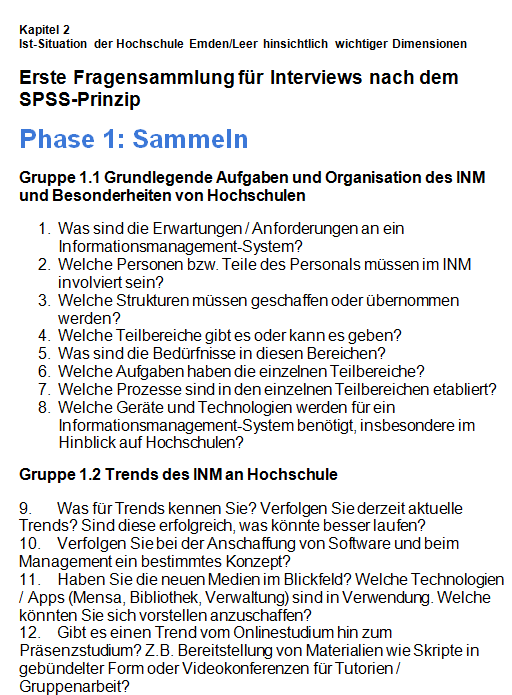
\includegraphics[width=10cm]{kapitel/gruppe2/bilder/auszug_fragen}
	\caption{Auszug der gesammelten Fragen}
	\label{fig_auszug_fragen_sammeln}
\end{figure}
Nach erfolgter Sammlung aller Fragen folgte im zweiten Schritt die Prüfung dieser Fragen. Hierbei wurden reine Informationsfragen aussortiert. Nach der erfolgreichen Prüfung der Fragen folgte im nächsten Schritt die Selektion von diesen. Die Fragestellungen wurden nach Themengebieten kategorisiert. Im letzten Schritt, dem Subsumieren des SPSS-Prinzips, wurde für jedes Themengebiet eine Erzählaufforderung gefunden und der Interviewleitfaden entsprechend diesen Erzählaufforderungen gegliedert. Mit Hilfe eines Farbcodes (siehe Abbildung \ref{fig_farbcode_SPSS}) wurden die Fragen entsprechend nach Erzählaufforderung, Checkliste, konkreter Frage und Aufrechterhaltungsfrage farblich markiert und anschließend einsortiert (siehe Abbildung \ref{fig_sortierung_fragentyp}).

\begin{figure}[h!]
	\centering
	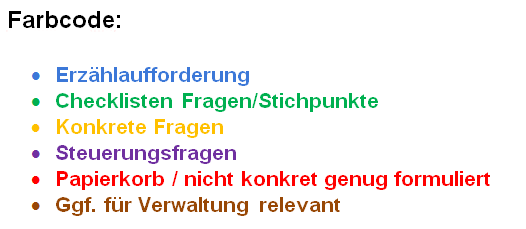
\includegraphics[width=10cm]{kapitel/gruppe2/bilder/farbcode_spss}
	\caption{angewandter Farbcode für das SPSS-Prinzip}
	\label{fig_farbcode_SPSS}
\end{figure}

\begin{figure}[h!]
	\centering
	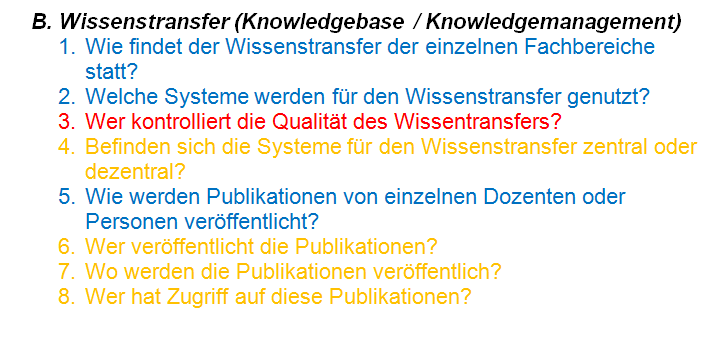
\includegraphics[width=10cm]{kapitel/gruppe2/bilder/sortierung_fragentyp}
	\caption{Sortierung der Fragen nach Fragentyp}
	\label{fig_sortierung_fragentyp}
\end{figure}

Diese Subsumtion wurde mit Hilfe des Anwendungsprogramms Microsoft Excel entsprechend visualisiert. Als Endergebnis  ist ein Interviewleitfaden entstanden, der in acht unterschiedliche Themenbereiche unterteilt wurde  (siehe Abbildung: \ref{fig_auszug_interviewleitfaden}).

\begin{figure}[h!]
	\centering
	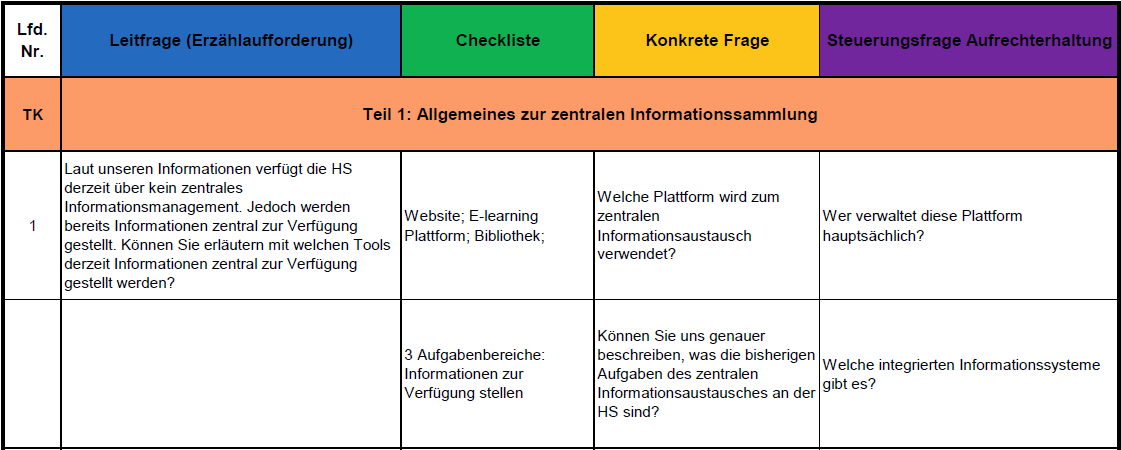
\includegraphics[width=10cm]{kapitel/gruppe2/bilder/auszug_leitfaden}
	\caption{Auszug des Interviewleitfadens}
	\label{fig_auszug_interviewleitfaden}
\end{figure}

An einem festgelegtem Interviewtermin ist mit Hilfe von diesem Leitfaden das Experteninterview mit Herrn Günter Müller durchgeführt worden. Dieses Interview fand mit der Online Video Plattform „Adobe Connect“ statt und wurde mit Zustimmung von Herrn Müller digital aufgezeichnet. Im Anschluss an das Experteninterview wurde in der ersten Phase die digitale Aufzeichnung auf wichtige inhaltliche Aspekte analysiert. 

In der zweiten Phase wurde durch Transkription die zur Verfügung gestellte Aufzeichnung, mit Hilfe der Applikation „Microsoft Word“, überführt um die im Interview erhaltenen Informationen besser verarbeiten zu können.

\begin{figure}[h!]
	\centering
	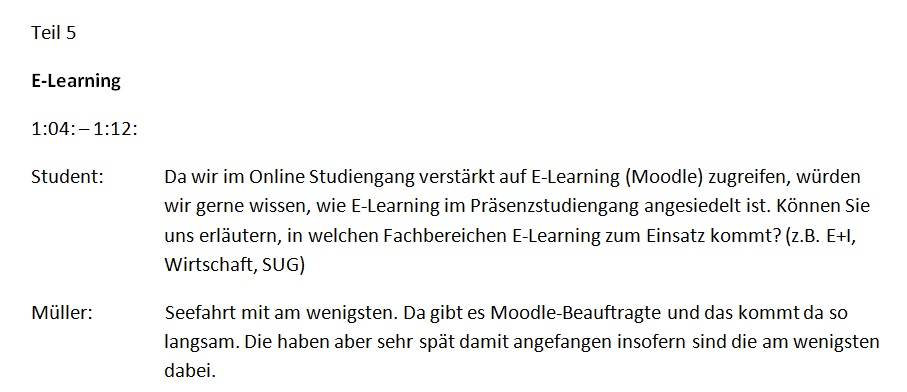
\includegraphics[width=10cm]{kapitel/gruppe2/bilder/E-Learning_Transkription}
	\caption{Transkription: E-Learning}
	\label{fig_E-Learning_Transkription}
\end{figure}

In der dritten und letzten Phase wurden mit Hilfe des Tools „XMind6“ zu jedem Themenbereich ein entsprechendes Mindmap generiert, um somit bei der Recherche schneller auf Besonderheiten eingehen zu können  (siehe Abbildung \ref{fig_E-Learning_MM}).

\begin{figure}[h!]
	\centering
	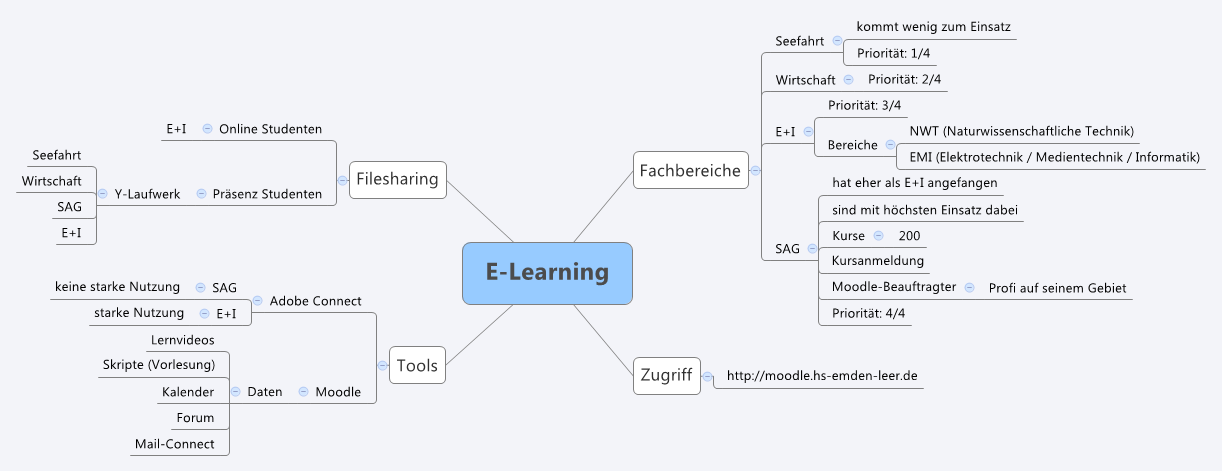
\includegraphics[width=10cm]{kapitel/gruppe2/bilder/E-Learning_MM}
	\caption{Mindmap: E-Learning}
	\label{fig_E-Learning_MM}
\end{figure}

Die Ergebnisse dieser Analyse werden in den folgenden Kapiteln detaillierter beschrieben. 

\section{Zuständigkeiten (TiK)}
\label{section_zustaendigkeiten}
In diesem Kapitel wird auf die Zuständigkeiten in Bezug auf die Informationsbereitstellung an der Hochschule Emden/Leer näher eingegangen. Es wird dargestellt, welche Bereiche bereits zentral an der Informationsbereitstellung beteiligt sind. Ebenso wird auf die Besonderheiten einzelner Fachbereiche, zentraler Einrichtungen und dem Präsidium detaillierter eingegangen (siehe Abbildung \ref{fig_organigramm_HS}). 

\begin{figure}[h!]
	\centering
	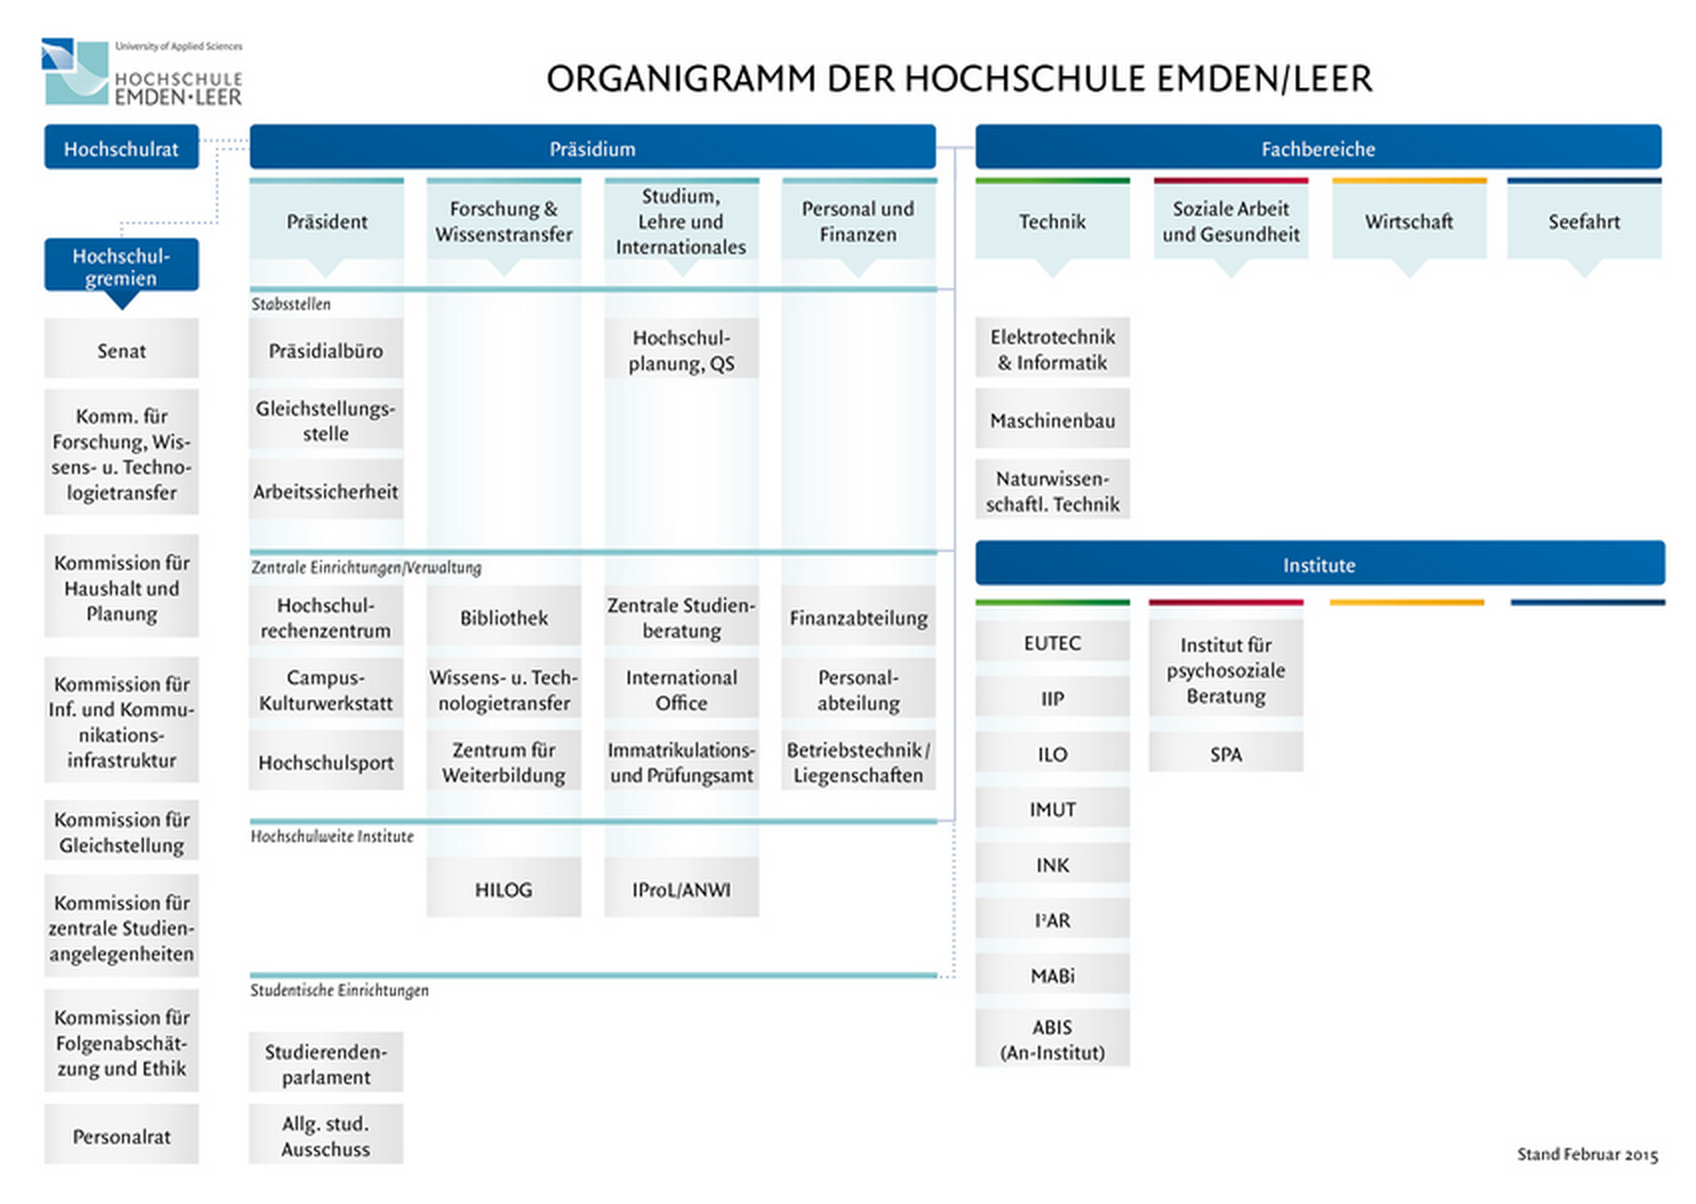
\includegraphics[width=14cm]{kapitel/gruppe2/bilder/organigramm_HS}
	\caption{Organigramm der Hochschule Emden/Leer}
	\label{fig_organigramm_HS}
\end{figure}

Nachfolgend wird ein Überblick über die IT-Systeme gegeben, welche sowohl von Mitarbeitern als auch Studierenden verwendet werden (siehe Abbildung  \ref{fig_zentrale_systeme}). Bei allen zentralen Systemen ist bereits eine Authentifizierung über Single Sign On (SSO) gegeben (siehe Kapitel \ref{realisierung_der_serviceorientierung} auf Seite \pageref{realisierung_der_serviceorientierung}).

\begin{figure}[h!]
	\centering
	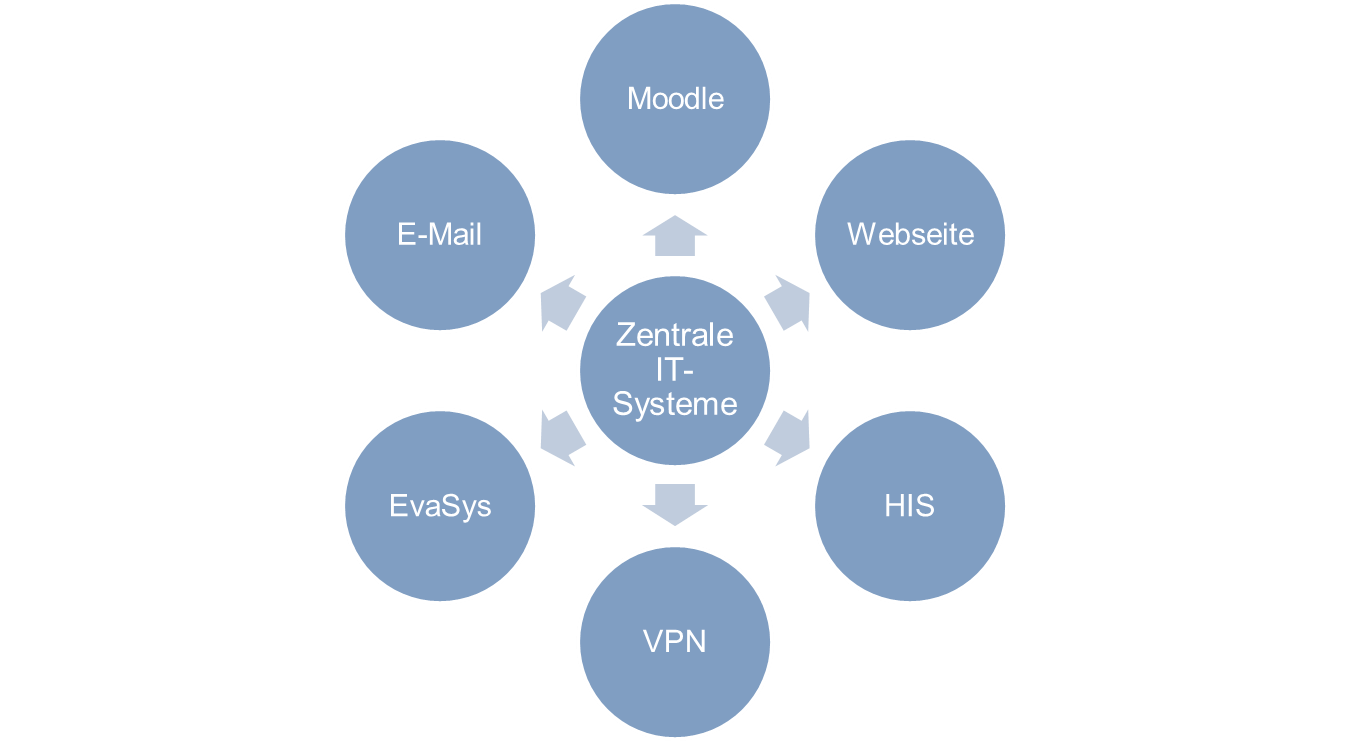
\includegraphics[width=14cm]{kapitel/gruppe2/bilder/zentrale_systeme}
	\caption{Zentrale Systeme für Mitarbeiter und Studenten}
	\label{fig_zentrale_systeme}
\end{figure}


\subsection{Fachbereiche}
Die einzelnen Fachbereiche sind unter anderem durch die Mitgliedschaft in Arbeitsgruppen in den Informationsbeschaffungsprozess involviert.

Alle Fachbereiche verfügen über die Berechtigung, relevante Informationen im Infosys darzustellen. Beim InfoSys handelt es sich um eine zentrale Plattform zur Darstellung von organisatorischen Informationen. Diese können direkt online auf der öffentlichen Webseite der Hochschule Emden/Leer eingesehen werden oder in den Eingangsbereichen der jeweiligen Fachbereiche vor Ort über entsprechende Monitore. Es werden, nach Fachbereich sortiert, die wichtigsten Neuigkeiten als Newsticker dargestellt und der Zugriff auf alle Vorlesungspläne der Fachbereiche ist gegeben, um so zügig auf organisatorische Inhalte zugreifen zu können (siehe Abbildung \ref{fig_InfoSys}). Aufbauend auf dem InfoSys wird eine selbst entwickelte Android App zur Verfügung gestellt.

\begin{figure}[h!]
	\centering
	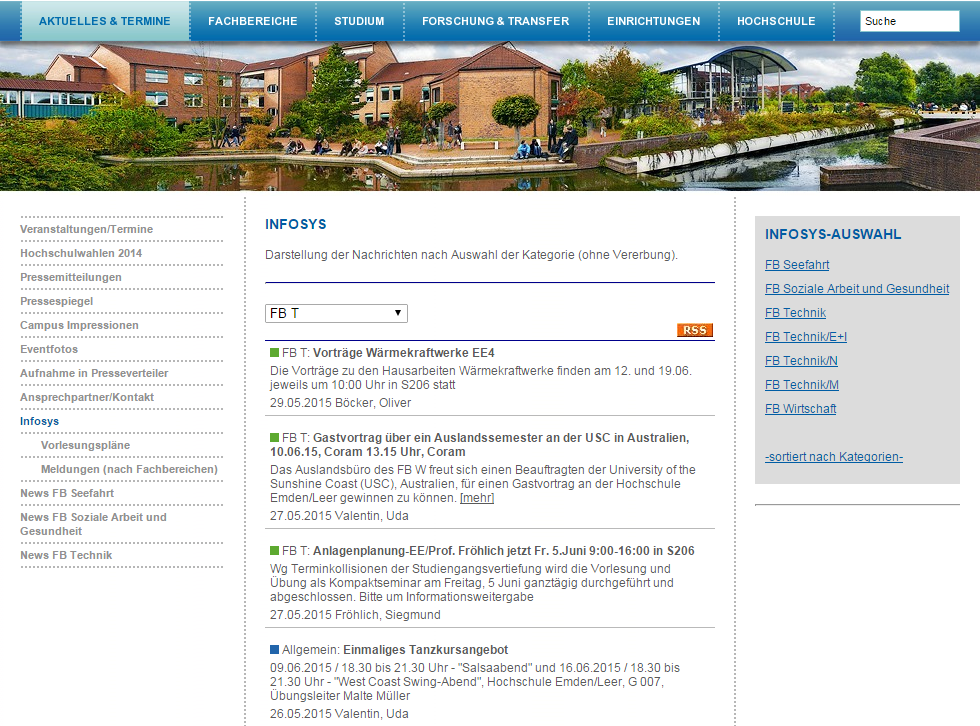
\includegraphics[width=14cm]{kapitel/gruppe2/bilder/InfoSys}
	\caption{Exemplarischer Screenshot des INFOSYS des Fachbereiches Technik}
	\label{fig_InfoSys}
\end{figure}

In den nachfolgenden Kapiteln wird auf die Besonderheiten der einzelnen Fachbereiche eingegangen.

\subsubsection{Seefahrt}
Bei dem Fachbereich Seefahrt handelt es sich um einen relativ kleinen Fachbereich. Seefahrt ist  nur am Standort Leer vertreten. Dieser Fachbereich verwendet kein zentrales System zur Vorlesung und Raumplanung, sondern eine Eigenentwicklung.

\subsubsection{Technik}
Eine Besonderheit dieses Fachbereiches ist es, dass für den Laborbetrieb ein Netzwerk neben dem zentralen Netzwerk der Hochschule Emden/Leer betrieben wird. Da unter anderem der Bereich „IT-Sicherheit“ ein wichtiger Aspekt in dem Studiengang Informatik ist, kommt es zu besonderen Konstellationen im Bereich der Forschung. Dieser Bereich verwaltet sein Netz selbst und ist somit autark vom allgemeinen Hochschulrechennetz. Es besteht jedoch eine enge Zusammenarbeit zwischen dem Bereich Technik (im speziellen E+I) und dem Rechenzentrum, so dass unter anderem gegenseitige Zugriffsrechte bestehen. 

\subsection{Präsidium}
\label{praesidium_label}

Die Hochschule Emden/Leer setzt Moodle als Lernplattform ein (siehe Abbildung 
Das Präsidium, insbesondere mit dem Bereich zentrale Verwaltung, ist über  Arbeitsgruppen in den Informationsbeschaffungsprozess involviert. Zudem verfügt das Präsidium mit einer Stabsstelle über einen zentralen Bereich im Bezug auf die Repräsentation von Informationen.  Das Präsidialbüro ist unter anderem für den Bereich Hochschulmarketing zuständig. Auch ist in der Stabstelle des Präsidialbüros die Presse- und Öffentlichkeitsarbeit angesiedelt.

\subsection{Zentrale Verwaltung}
Die zentrale Verwaltung verwendet im Bereich Personalverwaltung und Finanzen ausschließlich „SAP“ als Buchhaltungssystem. Zur Organisation von Lehr- und Vorlesungsplanung wird das System UNTIS Plus verwendet. Ebenso wird für die Urlaubsplanung, Zeiterfassung und das Gebäudeschließsystem ein eigenständiges System verwendet. Speziell für die Aufbereitung von Kennzahlen und Zahlen wird eine Eigenentwicklung als BIS (Business Intelligence System) verwendet. 

\subsubsection{Rechenzentrum}
Das Hochschulrechenzentrum der Hochschule ist stark in die Administration und Pflege der bestehenden Systeme zur Informationsbereitstellung involviert. Neben der Administration von bestehenden Systemen obliegt dem Hochschulrechenzentrum ebenfalls der Endkundensupport.

\subsection{Arbeitsgruppen zum Informationsaustausch und zur Informationsbereitstellung}
\label{subsection_arbeitsgruppen_informationsaustausch}
Die Zuständigkeiten an der Hochschule, in Bezug auf Informationssammlung, Beschaffung und Aufbereitung von Informationen, ist bereits durch Arbeitsgruppen in wichtigen Bereichen geregelt. Durch das Interview mit dem Leiter des Hochschulrechenzentrums konnte ein Einblick in die bestehenden Gremien geschaffen werden. Diese treffen sich regelmäßig zum Informations-, Wissens- und Erfahrungsaustausch.

Es existieren drei Arbeitsgruppen, welche für die Informationsverteilung in den jeweiligen Bereichen relevant sind:

\begin{itemize}
	\item Zahlen, Daten und Fakten (ZDF)
	\item WEB
	\item Moodle
\end{itemize}

\subsubsection{Zahlen, Daten und Fakten (ZDF)}
ZDF setzt sich zusammen aus den Verwaltungsabteilungen Finanzen, Personal, Presse und Rechenzentrum. Dieses Gremium ist zuständig für die Erstellung und Aufbereitung von Kennzahlen. Dies können zum Beispiel aktuelle Kennzahlen zu eingeschriebenen Studierenden pro Studiengang sein.  ZDF ist für einen Unterbereich der offiziellen Webseite der Hochschule zuständig. Die Kennzahlen und Zahlen werden gruppenbasiert erstellt. Je nach Berechtigung werden Kennzahlen in unterschiedlichen Detailgraden dargestellt. So erhalten Dekane mehr Informationen als Mitarbeiter. Öffentlich zugänglich sind nur generische Kennzahlen. 

\subsubsection{WEB}
Es existiert eine Arbeitsgruppe, welche für die Gestaltung und den Inhalt der öffentlichen Webseite der Hochschule verantwortlich ist. In dieser Arbeitsgruppe sind aus jedem Fachbereich Repräsentanten mit einbezogen. Die Leitung des Web-Teams obliegt dem Präsidialbüro.\footnote{\url{http://www.hs-emden-leer.de/fileadmin/user_upload/Einrichtungen/Praesidialbuero/Organigramm_Praesidialbuero_Juli2013_01.pdf}}

\subsubsection{Moodle}
In der Arbeitsgruppe „Moodle“ sind sowohl Repräsentanten aus jedem Fachbereich involviert sowie auch Repräsentanten aus der Verwaltungsebene. Da das Moodle E-Learning System mittlerweile als ein zentrales Moodle für alle Bereiche eingeführt wurde, haben die Mitglieder aus den Fachbereichen unter anderem das Recht, Kurse im Moodle freischalten zu können. Auf die E-Learning Plattform „Moodle“ wird detaillierter im Kapitel \ref{paragraph_moodle} auf Seite \pageref{paragraph_moodle} eingegangen.

\section{Definierte und bestehende Prozesse (Regelung und Handhabung von vorhandenen Informationen)(MaE)}

\subsection{Wissensmanagement}
Wissensmanagement ist für die Hochschule Emden/Leer ein sehr wichtiger Aspekt, da sie täglich mit dem Erwerb, der Entwicklung, dem Transfer sowie der Nutzung von Wissen konfrontiert wird. Für den Betrieb eines erfolgreichen Wissensmanagements ist ein klares Regelwerk die Voraussetzung.

\subsection{E-Learning}
E-Learning ist das Lehren und Lernen, welches durch elektronische Medien unterstützt wird. Zum Einsatz kommen digitale Medien, wie zum Beispiel Computer, Smartphones, aber auch das Internet dient als Konsummedium.\footnote{\url{http://team025.jimdo.com/unsere-vision/e-learning-eine-lernmethode-des-21-jahrhunderts/was-bedeutet-e-learning-eigentlich/}}

\subsubsection{E-Learning an der Hochschule Emden/Leer}
E-Learning ist an der Hochschule Emden/Leer ein sehr wichtiges Thema, da die Studiengänge Medieninformatik (Online) und seit 2015 Wirtschaftsinformatik (Online) akkreditiert  wurden. Nun soll dargelegt werden, ob in den Präsenzstudiengängen ebenfalls das Thema E-Learning Einzug gehalten hat.

\subsubsection{E-Learning in den Präsenzstudiengängen}
Es soll betrachtet werden, in welchen Präsenzstudiengängen E-Learning eingesetzt wird.

Der Fachbereich SAG (Soziale Arbeit und Gesundheit) ist der Vorreiter aller Fachbereiche mit der Einführung eines E-Learning Systems. SAG setzt mehr als 200 Onlinekurse im Präsenzstudium ein. Auch für die Anmeldung an verschiedenen Kursen kommt ein Online-System zum Einsatz.

Es folgt dann der Fachbereich Technik, in dem E-Learning ebenfalls sehr stark verbreitet ist, da die Studiengänge Medieninformatik und Wirtschaftsinformatik als reine Onlinestudiengänge in diesem integriert sind.

Weniger stark wird E-Learning vom Fachbereich Wirtschaft betrieben. Das geringste Nutzungsverhalten ist im Fachbereich Seefahrt zu verzeichnen.

Trotz des unterschiedlichen Nutzungsverhaltens hat E-Learning in allen Fachbereich Einzug gehalten.

\subsubsection[Einsatz von E-Learning-Anwendungen]{Einsatz von E-Learning-Anwendungen in den Präsenzstudiengängen}
In diesem Abschnitt wird erläutert, ob die Anwendungen Adobe Connect und Moodle im Präsenzstudiengang eingesetzt werden.

\paragraph{Adobe Connect}\mbox{} \\

Adobe Connect ist eine Kommunikationsplattform zur Bereitstellung von Webmeetings -und E-Learning-Inhalten.

Ausschließlich der Fachbereich Technik (E+I) nutzt durch seine Onlinestudiengänge die Plattform Adobe Connect als Medium des visuellen Austausches von Bild und Sprache. In den Präsenzstudiengängen kommt die Plattform nicht zum Einsatz, da der persönliche Austausch von Studierenden und Dozenten in den täglichen Präsenzen stattfindet.

\paragraph{Moodle}\mbox{} \\

Die Hochschule Emden/Leer setzt Moodle als Lernplattform ein (siehe Abbildung 5.6). Moodle ist ein freies objektorientiertes Kursmanagementsystem, welches prädestiniert ist für den Einsatz von E-Learning Inhalten.\footnote{\url{https://moodle.hs-emden-leer.de/moodle/}}

\begin{figure}[h!]
	\centering
	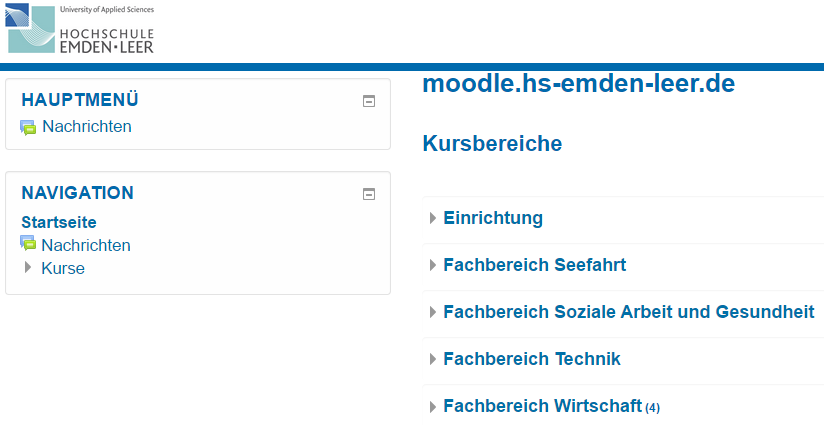
\includegraphics[width=8cm]{kapitel/gruppe2/bilder/moodle}
	\caption{Übersicht Moodle für alle}
	\label{fig_moodle}
\end{figure}

Durch den Einsatz von Moodle in allen Fachbereichen, wird das volle Leistungsspektrum des Systems ausgenutzt. Folgende Funktionalitäten werden angeboten:
\begin{itemize}
	\item Lernvideos
	\item Vorlesungsskripte
	\item Forum
	\item Kalender
	\item Mail-Connect
\end{itemize}

Für jeden Fachbereich wird der volle Funktionsumfang der Plattform zur Verfügung gestellt, auch wenn nicht jeder Fachbereich jeden Service nutzt. 

\subsubsection{Zentrale Informationsbereitstellung durch Datenlaufwerke}
Für alle beteiligten der Hochschule Emden/Leer werden drei Datenlaufwerke (siehe Abbildung 5.7) auf den Fileservern der Hochschule zur Verfügung gestellt.\footnote{\url{https://connect.hs-emden-leer.de/cgi-bin/portal}}

\begin{figure}[h!]
	\centering
	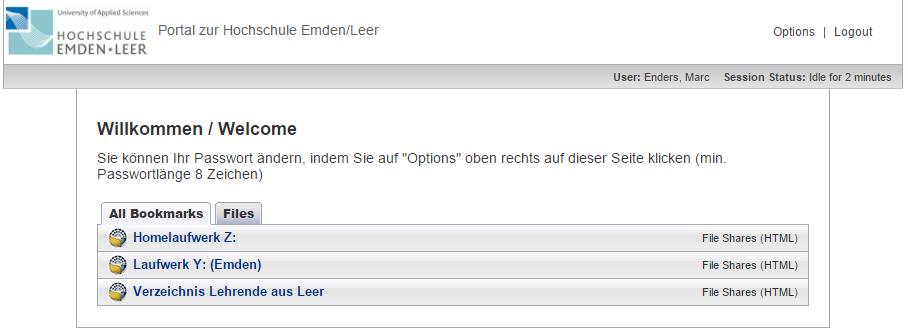
\includegraphics[width=8cm]{kapitel/gruppe2/bilder/zugriff_auf_laufwerke_extern}
	\caption{Zugriff auf die Datenlaufwerke von extern}
	\label{fig_zugriff_datenlaufwerke_extern}
\end{figure}


\paragraph{Laufwerk Z}\mbox{} \\

Auf dem Laufwerk Z befinden sich die Daten des Home-Verzeichnisses jedes einzelnen Benutzers. Meldet sich dieser an beliebigen Rechnern des Rechnerpools an, werden die Inhalte Ihres Home-Verzeichnisses automatisch eingebunden. Der interne Zugriff auf die eigenen Dateien ist von jedem Rechner des Pools möglich, da servergespeicherte Profile zum Einsatz kommen. Auch von extern können die Studierenden problemlos auf die Ressourcen der Datenlaufwerke zugreifen.

\paragraph{Laufwerk Y}\mbox{} \\

Für den gemeinsamen Austausch der Daten wurde das Transferlaufwerk Y eingerichtet. Hier werden zentral Ressourcen für alle Studierenden und Lehrenden aus Emden zum Austausch zur Verfügung gestellt.

\paragraph{Verzeichnis Lehrende aus Leer}\mbox{} \\

Zusätzlich zum Transferlaufwerk steht das Verzeichnis der Lehrenden aus Leer  zur Verfügung. Dieses Laufwerk wird zur Bereitstellung von Inhalten, wie zum Beispiel Vorlesungsmaterialien, verwendet.

\subsubsection{Moodle vs. Datenlaufwerke für Präsenzstudenten}
An der Moodle-Plattform melden sich die Nutzer über eine webbasierte Oberfläche am System an. Um Dateien zur Verfügung zu stellen, muss auf der Weboberfläche zu den gewünschten Reitern navigiert werden.

Stellt man die Datenlaufwerke (Y Laufwerk und Transferlaufwerk der Lehrenden aus Leer) der Moodle-Plattform gegenüber und betrachtet nur den Aspekt des Datenaustausches, so wird deutlich, dass der Dateiaustausch über   Datenlaufwerke in Bezug auf Komfort und Aufwand deutlich besser für die Präsenzstudierenden geeignet ist, als die Dateiablage über die Moodle-Plattform. Die über die Datenlaufwerke zur Verfügung gestellten Inhalte können von den Studierenden mit wenig Aufwand intuitiv erreicht werden.

Aus dem Interview mit dem Rechenzentrumsleiter Herrn Günter Müller kristallisierte sich heraus, dass der Fachbereich Wirtschaft die Datenlaufwerke am stärksten und der Fachbereich Technik und andere Fachbereiche diese weniger stark nutzen.

\subsection{Sicherheitsaspekte}
In diesem Kapitel wird auf die bereits verwendeten Sicherheitsrichtlinien und dem IT-Service-Management (ITSM)  Prozess an der Hochschule Emden/Leer detaillierter eingegangen.

\subsubsection{Sicherheitsrichtlinien an der Hochschule Emden / Leer}
Der Einsatz von Sicherheitsrichtlinien ist ein wichtiges Thema an Hochschulen. Sicherheitsrichtlinien beschreiben die Sicherstellung von Verfügbarkeit, Integrität, Vertraulichkeit und Authentizität von Informationen.
An der Hochschule Emden/Leer werden als Basis für die Informationssicherheit Teile des IT-Grundschutz-Kataloges umgesetzt. Nicht alle Empfehlungen des BSI sind an einer kleinen Hochschule, wie die Hochschule Emden/Leer es ist,  umsetzbar.

An den Serverräumen der Hochschule ist die Umsetzung der IT-Grundschutzmaßnahmen deutlich zu erkennen.
Folgende physikalische Schutzmaßnahmen wurden an der Hochschule Emden/Leer in den Serverräumen umgesetzt:

\begin{itemize}
	\item einbruchssicher
	\item feuergemeldet
	\item videoüberwacht
	\item Lage der Serverräume im 1. OG (Wasserschutz)
\end{itemize}

\subsubsection{Einsatz von ITIL}
Die IT Infrastructure Libary (ITIL) ist eine Sammlung von Best Practises zur Umsetzung eines IT-Service-Managements (ITSM). In diesem Regelwerk werden die für den Betrieb einer IT-Infrastruktur notwendigen Prozesse und Werkzeuge beschrieben.\footnote{\url{http://wirtschaftslexikon.gabler.de/Definition/itil.html}}

Der ITIL-Prozess ist an der Hochschule Emden/Leer nicht etabliert, da die Personaldecke für die Umsetzung eines 1st- und 2nd-Level Supports nicht gegeben ist.

\subsubsection{Umsetzung von ISO/IEC 27001}
Die ISO/IEC 27001 Zertifizierung wird auf Basis des IT-Grundschutzes vergeben. Durch die Zertifizierung des ISO/IEC 27001 Standards haben Unternehmen, Behörden und Organisationen die Möglichkeit, ihre Bemühungen um Informationssicherheit nach innen und außen zu dokumentieren.\footnote{\url{https://www.bsi.bund.de/DE/Themen/ZertifizierungundAnerkennung/Zertifizierung27001/GS_Zertifizierung_node.html}}

Das Einsatzszenario ist an der Hochschule Emden/Leer nicht gegeben, da für Umsetzung die Personaldichte zu gering ist. Für die Erfüllung der Zertifizierung würde ein riesiger Personaloverhead entstehen.

\subsubsection{Fazit Sicherheitsrichtlinien}
Abschließend ist zu sagen, dass an der Hochschule Emden/Leer der IT-Sicherheitsaspekt ein sehr wichtiges Thema ist. Als kleine Hochschule ist es auf Grund der Personaldichte nicht möglich, alle Empfehlungen des BSI-Grundschutzes, ITIL und ISO/IEC 27001 umzusetzen. Jedoch sucht sich die Hochschule aus den Regelwerken die Empfehlungen heraus, die auf Grund der Personaldichte umsetzbar sind.  Dies bildet eine sehr gute Basis im Hinblick auf das sehr anspruchsvolle Thema IT-Sicherheit.


\section{Repräsentation von Informationen}
\section{Kooperations-Situation mit anderen Hochschulen (MaE)}
\label{section_kooperations_situation}

Kooperationsverhältnisse mit anderen Hochschulen, Verbänden und Unternehmen spielen auch an der Hochschule Emden/Leer eine sehr entscheidende Rolle, da durch die Kooperation verschiedene Services zur Verfügung gestellt werden.

\subsection{Regionaler Bezug zu Hochschulen (Mitgliedschaften)}
Die Hochschule Emden/Leer pflegt ein enges Kooperationsverhältnis mit dem Jade-Hochschulverbund. Über das Lokale Bibliothekssystem Ostfriesland/Wilhelmshaven (LBS) wird auf die gemeinsamen  Bibliotheksbestände zugegriffen.\footnote{\url{http://www.jade-hs.de/service-verwaltung/hochschulbibliothek/bestand/online-kataloge/}}

Durch ein gemeinsames Promotionskolleg findet ebenfalls eine intensive Zusammenarbeit mit der Universität Vechta statt. Aktuell baut die Hochschule Emden/Leer die Kooperation zur Hochschule Osnabrück aus.\footnote{\url{http://www.hs-emden-leer.de/hochschule/profil.html}}

Der Rechenzentrumsleiter Herr Günter Müller ist selbst Mitglied des Arbeitskreises LANIT/HRZ. Hier treffen die Leiter der Rechenzentren Niedersachsens aufeinander und tauschen Ihre Erfahrungen aus. Der Arbeitskreis befasst sich mit Themen der IT-Infrastruktur für Forschung, Lehre und Verwaltung an den Hochschulen Niedersachsens. Zu Schwerpunktthemen wurden Arbeitsgruppen eingerichtet.  Ebenfalls werden hochschulübergreifend Projekte durchgeführt.\footnote{\url{http://www.lanit-hrz.de/}}

Das ZKI (Zentren für Kommunikation und Informationsverarbeitung in Lehre und Forschung e.V.) spielt für die Hochschule eine wichtige Rolle. Ziel dieses Vereins ist es, die Kooperation zwischen den ZKI/Rechenzentren, Meinungs- und Erfahrungsaustausch, sowie die Beratung und Zusammenarbeit mit bildungs- und wirtschaftsfördernden Einrichtungen zu fördern. In den immer wiederkehrenden Tagungen erarbeitet der Arbeitskreis Lösungsvorschläge für aktuelle Probleme der Informationsverarbeitung. Aktuelle Themen sind z.B. eine Studie über das Thema: „CIOs und IT-Governance an deutschen Hochschulen“.\footnote{\url{https://www.zki.de/zki-nachrichten/einzelbeitrag/1215/}}

Durch den Verein DFN (Deutsches Forschungsnetz) wird der Hochschule eine Vielzahl von maßgeschneiderten Kommunikationsanwendungen (DFN-Diensten) zur Verfügung gestellt. Der DFN-Verein ist ein von der Wissenschaft selbst organisiertes Kommunikationsnetz für Wissenschaft und Forschung in Deutschland. Er verbindet Hochschulen und Forschungseinrichtungen miteinander und ist in den europäischen und weltweiten  Verbund der Forschungsnetze integriert.\footnote{\url{https://www.dfn.de/}}

\subsection{Kooperation zwischen Unternehmen}
Regional betrachtet arbeitet die Hochschule Emden/Leer mit 82\% der Unternehmen der Region zusammen. Der Vorteil dieser Kooperation ist es, dass zum Einen die Studierenden die Möglichkeit haben ihre Fähigkeiten in der Praxis anzuwenden und zum Anderen können die Unternehmen das Know-How  der Hochschule nutzen und sinnvoll einsetzen. Der Wissenstransfer, der in der Hochschule erfolgt, bietet den Unternehmen einen erheblichen Mehrwert.\footnote{\url{http://www.hs-emden-leer.de/en/news-events/news/article/hochschule-weit-vorn-bei-kooperation-mit-unternehmen.html}}

\subsection{Eingesetzte IT-Systeme durch Mitgliedschaft im DFN-Verein}
Die angebotenen Dienste des Deutschen Forschungsnetzes sind für den Zweck von Wissenschaft und Forschung maßgeschneidert worden. Ein besonderes Augenmerk liegt hier auf der guten Integration der Dienste in die Prozesse der Hochschulen.  Auf die über den DFN-Verein zur Verfügung gestellten Dienste, die an der Hochschule Emden/Leer zum Einsatz kommen, wird folgend näher eingegangen.\footnote{\url{https://www.dfn.de/dienstleistungen/}}

\subsubsection{DFNRoaming/eduroam}
Die Hochschule Emden/Leer ist Mitglied des Deutschen Forschungsnetzes (DFN). Durch diese Kooperation nutzt die Hochschule den durch das DFN zur Verfügung gestellten Dienst DFNRoaming/eduroam. Dieser ermöglicht es, registrierten Nutzern über dienst-konforme WLANs Zugang zum Wissenschaftsnetz zur Verfügung zu stellen. Der DFN-Verein betreibt und pflegt die eduroam Förderationsserver in Deutschland. \footnote{\url{https://www.dfn.de/dienstleistungen/dfnroaming/}} 

In der Übersicht ist ein Ausschnitt von Lokalitäten einiger Förderationsserver weltweit dargestellt (siehe Abbildung 5.10).\footnote{\url{http://weill.cornell.edu/its/images/eduroam-map.jpg}}

\begin{figure}[h!]
	\centering
	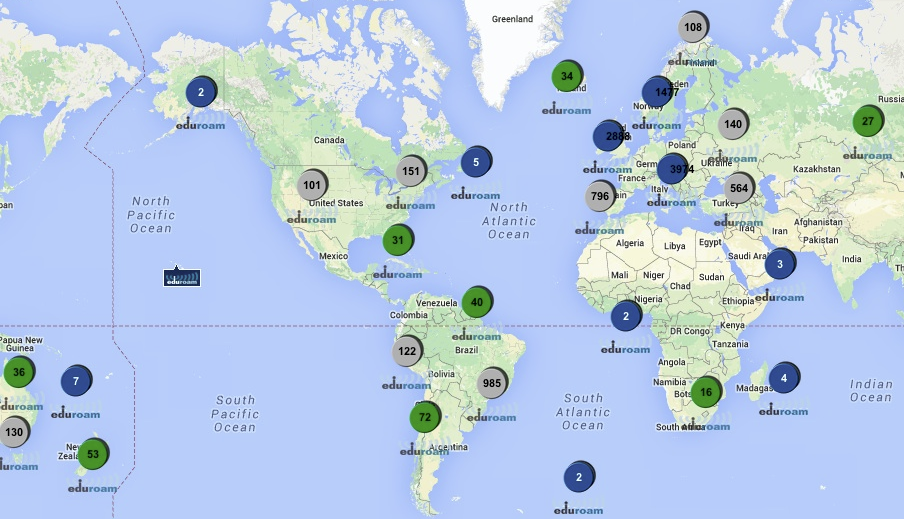
\includegraphics[width=8cm]{kapitel/gruppe2/bilder/eduroam_map}
	\caption{Standorte an denen das DFNRoaming/eduroam betrieben wird}
	\label{fig_map_eduroam}
\end{figure}

\subsubsection{GigaMove der RWTH Aachen}
Die Rheinisch-Westfälische Technische Hochschule Aachen (RWTH Aachen) stellt eine einfach zu nutzende Möglichkeit zum kurzfristigen Austausch großer Dateien zur Verfügung. Der Datenaustausch kann aus zwei Richtungen angestoßen werden. Zum Einen kann ein Nutzer eine Datei hochladen und die Anwendung erzeugt einen Link zum Download, zum Anderen kann eine Datei angefordert werden, bei der die Anwendung einen Link generiert, der zu einem Formular zum Upload der Datei führt. Jeder Nutzer darf standardmäßig Dateien in der Gesamtgröße von 10 GB für einen Zeitraum von 14 Tagen auf den gehosteten Servern abspeichern. Der von der RWTH Aachen gehostete Dienst GigaMove wird den Nutzern der Hochschule Emden/Leer zur Verfügung gestellt. In der Abbildung 15 ist die Plattform GigaMove der RWTH Aachen dargestellt. \footnote{\url{https://gigamove.rz.rwth-aachen.de/}} 

\begin{figure}
	\centering
	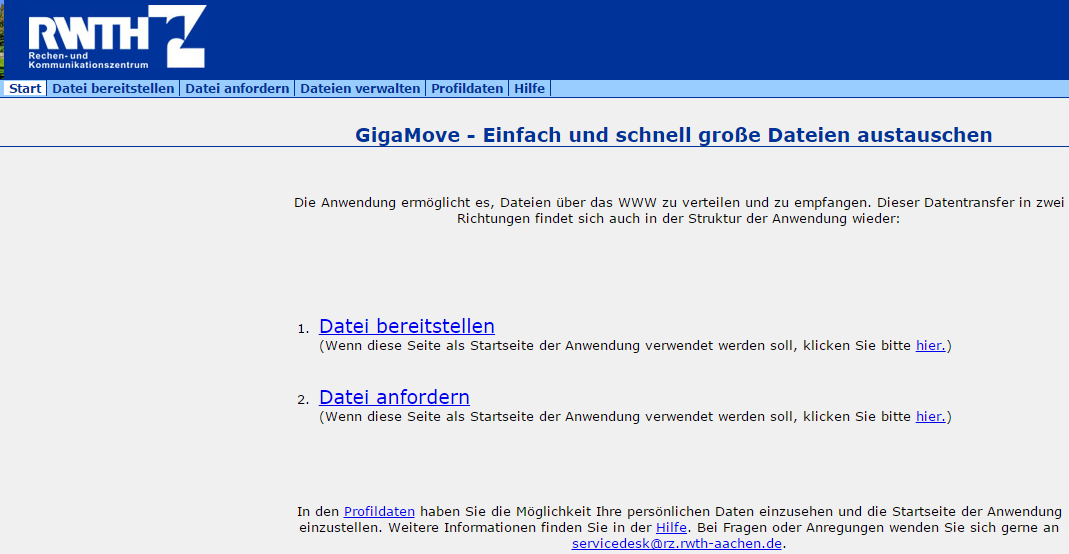
\includegraphics[width=8cm]{kapitel/gruppe2/bilder/rwth_gigamove}
	\caption{Übersicht der Plattform GigaMove der RWTH Aachen}
	\label{fig_rwth_gigamove}
\end{figure}

\subsubsection{DFNVideoConference (DFNVC)}
DFVNC bietet den Nutzern die Möglichkeit von einem PC, einem Raumsystem oder einem Telefon durch Nutzung des Wissenschaftsnetzes X-WiN mit einem oder mehreren Nutzern zu kommunizieren. Die Kommunikation findet multimedial statt. Das Wissenschaftsnetz X-WiN ist die technische Plattform des Deutschen Forschungsnetzes. Über das X-WiN sind die Hochschulen und Forschungseinrichtungen in Deutschland untereinander und mit den Wissenschaftsnetzen in Europa auf anderen Kontinenten vernetzt.\footnote{\url{https://www.dfn.de/dienstleistungen/dfnvc/}} An der Hochschule wird dieser Dienst ebenfalls genutzt.

\subsection{Authentifizierung über das Shibboleth-Verfahren}
Das von der Hochschule eingesetzte Shibboleth-Verfahren ermöglicht den Studierenden und Mitarbeitern Ressourcen der Anbieter SpringerLink, WISO, video2brain und andere Dienste zu nutzen. Hierbei muss bei der Anmeldung die Hochschule als Heimatinstitution und die Hochschulkennung angegeben werden.\footnote{\url{http://www.hs-emden-leer.de/no_cache/einrichtungen/bibliothek/medienangebot/elektronische-angebote/vpn-shibboleth.html}}

\subsubsection{Springer Link}
Studierende und Mitarbeiter der Hochschule Emden/Leer haben über die Springer Link-Kooperation Zugriff auf über 40.000 Bücher, 5 Millionen Artikel, 2200 Zeitschriften und 165 Nachschlagewerk.\footnote{\url{http://link.springer.com/athens-shibboleth-login}} Die Oberfläche der Springer Link Plattform ist in Abbildung 5.12 zu sehen. Springer Link bietet die Möglichkeit die Inhalte als *.pdf herunterzuladen. 

\begin{figure}[h!]
	\centering
	
\includegraphics[width=8cm]{kapitel/gruppe2/bilder/springerlink_startseite}
	\caption{Springer Link Startseite}
	\label{fig_springerlink_startseite}
\end{figure}

\subsubsection{WISO}
Durch das Kooperationsverhältnis mit der GBI-Genios Deutsche Wirtschaftsdatenbank GmbH können die Mitglieder der Hochschule Emden/Leer das komplette Angebot an Fachinformationen zu den Wirtschafts- und Sozialwissenschaften, zu technischen Studiengängen und zur Psychologie  nutzen. WISO bietet über 14 Mio. Literaturnachweise, 2100 elektronische Bücher, 130 Mio. Artikel, 700.000 Marktdaten.\footnote{\url{https://www.wiso-net.de/popup/ueber_wiso}}

\begin{figure}[h!]
	\centering
	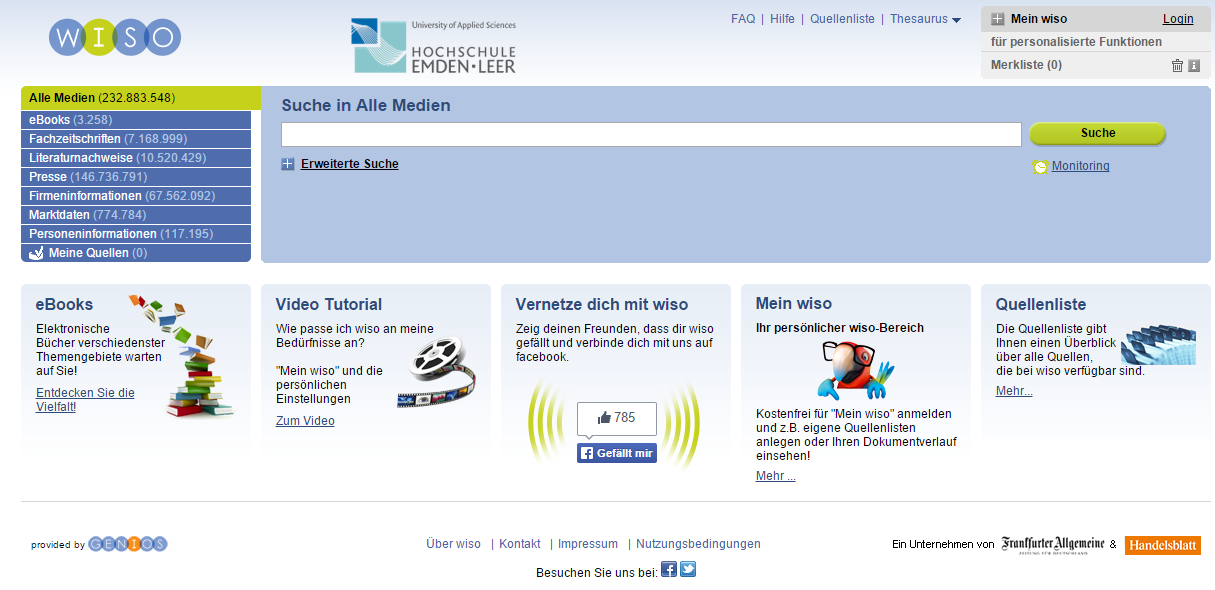
\includegraphics[width=8cm]{kapitel/gruppe2/bilder/wiso_plattform.png}
	\caption{Übersicht der WISO Plattform}
	\label{fig_wiso_plattform.png}
\end{figure}

\subsubsection{video2brain}
Seit 2015 ist für alle Mitarbeiter und Studierende der Zugang zum Videostreaming-Portal der video2brain GmbH möglich. Schwerpunkt sind IT- und Kreativ-Themen, Lehrvideos für Fotografen, Grafiker, Web- und Screendesigner. Das Verlagsangebot umfasst mehr als 1700 Video-Trainingskurse. In der Abbildung 5.14 ist die Weboberfläche nach erfolgreicher SSO-Authentifizierung dargestellt.\footnote{\url{https://www.video2brain.com/de/}}

\begin{figure}[h!]
	\centering
	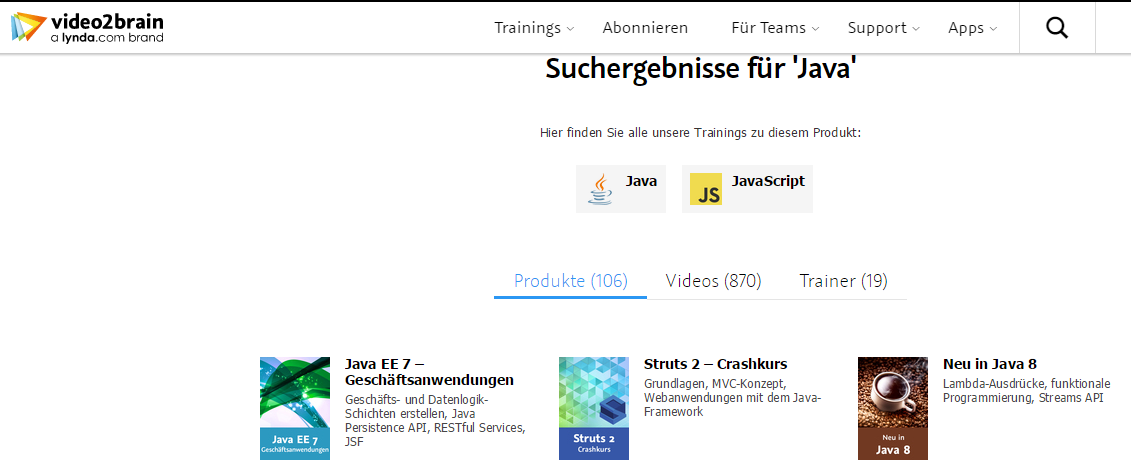
\includegraphics[width=8cm]{kapitel/gruppe2/bilder/video2brain_suche}
	\caption{Übersicht der video2brain Plattform}
	\label{fig_video2brain_suchergebnis}
\end{figure}

\subsection{Support der Dienste}
Für die zentral angebotenen Dienste eduroam, Shibboleth und GigaMove übernimmt die Hochschule Emden/Leer den Endkundensupport. Die Mitarbeiter der Hochschule Emden/Leer bilden somit die zentrale Support-Schnittstelle und delegieren Anfragen, die vor Ort nicht gelöst werden können, an die entsprechenden Anbieter weiter.

Diese Informationen teilte uns der Leiter des Hochschulrechenzentrums Emden/Leer, Herr Günter Müller in dem durchgeführten Interview mit.
\section{Bewertung und Gewichtung (TiK)}
Abschließend kann gesagt werden, dass Informationen zentral gesammelt werden und wichtige Systeme wie das "'Laufwerk Y"' und die E-Learning Plattform (Moodle) in allen Fachbereichen und in Teilen der Verwaltung zum Einsatz kommen. Durch den starken Kooperationsverbund werden zentrale Dienste, wie Springer Link, WISO und video2brain für die Studierenden und Mitarbeiter dezentral zur Verfügung gestellt. 

Bei der Repräsentation von Informationen nach außen verfügt die Hochschule über eine Pressestelle und eine Marketingabteilung. Es existiert eine feste CD-Reglung für alle Abteilungen und Bereiche. 

Durch diverse Arbeitsgruppen ist der Erfahrungs-, Wissens- und Informationsaustausch für wichtige zentrale Bereiche bereits gegeben. Durch die Arbeitsgruppe ZDF, WEB und Moodle werden zentrale Systeme zur Wissenserhaltung und Informationsbereitstellung gepflegt. Dadurch, das die Arbeitsgruppen abteilungsübergreifend agieren, besteht auch zwischen den einzelnen Bereichen eine Schnittstelle, ohne die autarken Fachbereiche einzuschränken. 

Im Bezug auf Serviceorientierung und IT-Sicherheit lässt sich sagen, dass SSO (Single-Sign-On) für einige Bereiche bereits zum Einsatz kommt (siehe Kapitel \ref{realisierung_der_serviceorientierung} auf Seite \pageref{realisierung_der_serviceorientierung}). Ebenso werden Teile des IT-Grundschutzes erfolgreich an der Hochschule eingesetzt. Dies sind erste Schritte zum Informationsmanagement, jedoch fehlt grundsätzlich ein zentrales System für den direkten Zugriff und zur Weiterleitung auf weitere Informationssysteme. In Kapitel \ref{immatrikulations_und_pruefungsamt} auf Seite \pageref{immatrikulations_und_pruefungsamt} wird beschrieben, dass in Hochschulen, welche ein Informationsmanagement einsetzen, dieses meistens im Bereich Immatrikulations- und Prüfungsamt (HIS) angesiedelt ist. 
Neben einem  zentralem System fehlt auf der organisatorischen Seite eine Instanz. Wie in Kapitel \ref{cio_text} auf Seite \pageref{cio_text} beschrieben, findet im klassischen Informationsmanagement für Unternehmen das Management häufig durch einen Chief Information Officer (CIO) statt. In Hochschulen wird dies oft durch DACH Organisationen realisiert. 

Auch wenn die Hochschule bereits diverse Arbeitsgruppen einsetzt, so ist diese Instanz des Informationsmanagements bisher unbesetzt. Ein Informationsmanagement, wie es in Kapitel \ref{begriffsdefintion_inm} auf Seite \pageref{begriffsdefintion_inm} beschrieben ist, wird derzeit an der Hochschule nicht vollständig praktiziert.
%\chapter{Mögliche Soll-Situation im Hinblick auf die heutigen und zukünftigen Aufgaben - AE, JL, HS}

\textit{Autoren: Andreas Ebling, Julia Lübke, Hannes Sprafke}

Ich bin ein Einleitungstext zu diesem Kapitel, der noch geschrieben werden muss.

\section{Marketing}
\label{section_marketing}
Das Marketing hat neben dem typischen Aufgabenbereich der Außenrepräsentation durch die Besonderheiten einer Hochschule auch einen Aufgabenbereich der Innenrepräsentation. Im folgenden werden diese Bereiche getrennt betrachtet.

\subsection{Externes Hochschulmarketing}
\label{subsection_externes_hochschulemarketing}
Das externe Marketing der Hochschule bezieht sich auf die klassischen Marketingaufgaben, das Produkt und die Marke vorteilhaft darzustellen. Im Falle einer Hochschule ist dies die attraktive Darstellung gegenüber zukünftige Studierenden, Forschungsinteressierten und Geldgebern.

\subsubsection{Webseite}
Zentrales Element bleibt die Hochschulwebseite, die mit aktuellen, offenen Möglichkeiten von HTML 5, CSS 3 und JavaScript den Funktionsumfang einer App erreichen kann, ohne auf spezielle oder spezifische Spezialtechnologien zu setzen. Besonders sei an dieser Stelle die Möglichkeit genannt, mittels CSS Größen und Darstellungsmöglichkeiten von Endgeräten unabhängig von konkreten Betriebssystemen und Hardwareplattformen abzudecken.

Dies ist vor dem Hintergrund wichtig, dass beispielsweise eine native App für iPhones zwingend durch den Appstore der Firma Apple installiert werden muss, dessen Nutzungsbedingungen sich für die Hochschule in Form von Kosten oder Inhaltseinschränkungen zu Ungunsten der Hochschule verändern könnten. Mit einer nativen App lässt sich trotzdem nur ein beschränkter Nutzerkreis ansprechen. Sollen mehrere Apps für verschiedene Plattformen gepflegt werden, so ist dies mit zusätzlichen Aufwand verbunden.

Eine Neuauflage der Hochschulwebseite mit aktuellen Möglichkeiten und per CSS an verschiedene Darstellungsgrößen angepasst erreicht dagegen jedes internetfähige Gerät mit Browser. Sollte ein neuer Formfaktor wichtig werden, zum Beispiel der einer Smartwatch, so lässt sich dies über eine Erweiterung des Stylesheets erreichen, ohne eine komplette Neuentwicklung in Auftrag zu geben.

\subsubsection{Soziale Netzwerke}
Soziale Netzwerke wie facebook oder twitter sind kritisch zu bewerten. Auftritte auf diesen Plattformen können nicht alleine stehen, benötigen aber durch ständigen Nutzerkontakt eigenständige Pflege und Aufsicht, was an einer kleinen Hochschule Personal bindet.

Der Nutzen ist weiterhin fraglich. Die Hochschule kann bestenfalls Informationen der Webseite duplizieren, während Kommunikation von Interessierten zur Hochschule wieder schnell in bestehende Kanäle geleitet wird.

Weiterhin ist die Reichweite zwar potentiell weltweit, was für eine nach Leitbild „Hochschule der Region“ aber an sich nicht relevant ist. In der Praxis wichtiger ist die Dichte der Nutzer, da es unrealistisch ist zu erwarten, dass jeder in sozialen Netzwerken organisiert ist, oder aber sich zur Nutzung in einem sozialen Netzwerk anmelden müsste.

Über interne Kommunikation und Daten in sozialen Netzwerken müsste im Einzelfall nach Grundlage geltender Datenschutzvorgaben entschieden werden, was als Prozess vorab bereits zu aufwendig, als dass eine Erwägung hier weiter Sinn machen würde.
Im Endeffekt verbliebe also die Verbreitung ohnehin öffentlicher Informationen, die bereits auf der Webseite zu finden wären.

\subsubsection{Verteilte Content-Erzeugung}
Im Kontext einer kleinen Hochschule ist die Personalsituation zu berücksichtigen. Es kann nicht davon ausgegangen werden, dass eine oder mehrere Personen die Redaktion aller zu veröffentlichenden Inhalte übernehmen. Vielmehr ist zu erwarten, dass relevante Neuigkeiten an mehreren unterschiedlichen Stellen auftreten, und am besten ohne Umweg veröffentlicht werden. Hierzu eignen sich Content-Management-Systeme.

\begin{figure}[h!]
	\centering
	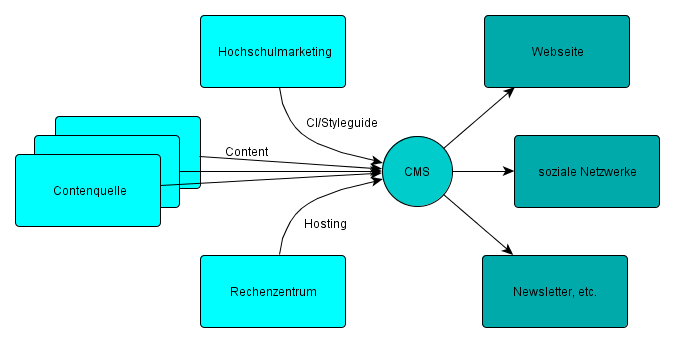
\includegraphics[width=10cm]{kapitel/gruppe3/bilder/verteilter_publishing_workflow}
	\caption{Verteilter Publishing Workflow}
	\label{fig_publishing_workflow}
\end{figure}

Mit diesen kann geleistet werden, dass mehrere, unabhängige Autoren Inhalte beisteuern und veröffentlichen können, ohne im Einzelnen mit den technischen Einzelheiten des Hostings oder des Designs belangt zu werden. Auch können vielfach Content Management Systeme Inhalte für weitere Plattformen aufbereiten, zum Beispiel an soziale Netzwerke posten.

\subsection{Internes Hochschulmarketing}
\label{subsection_internes_hochschulemarketing}
Im Gegensatz zur Situation in einem Unternehmen genießen einzelne Fachbereiche und Personen in einer Hochschule einen hohen Grad an Freiheit und Autonomie. Daher können in Arbeitsgruppen und Gremien beschlossene Prozesse und Software nicht per Anordnung durchgesetzt werden, sondern müssen nach innen vermarktet werden, um akzeptiert zu werden.Herausfordernd ist hier besonders die Heterogenität, da der technische und fachliche Hintergrund sich unter Mitarbeitern und Fachbereichen erheblich unterscheiden dürften, etwa zwischen technischen und nichttechnischen Fachbereichen.

\subsubsection{Fokussierter Support}
Eine Möglichkeit, Benutzer hin zu einer präferierten Lösung zu leiten ist diese in Präferenzen, Anleitungen und FAQs an erster Stelle und in höherem Detailgrad zu präsentieren. Vielfach wird eine Voreinstellung einfach übernommen, und die erste Lösung zu einer Fragestellung als Referenz angesehen.

\subsubsection{Schulungen}
Eine weitere Maßnahme ist, Schulungen für die präferierten Lösungen anzubieten, die Vorteile der gefundenen Lösung gegenüber anderen herausstellt. Optimal ist eine solche Lösung transparent, oder aber bietet Alleinstellungsmerkmale, die eine Verwendung aus sich heraus attraktiv erscheinen lassen. Trotzdem kann es vorkommen, dass in Lern- und Umstellungsphasen Lernkurven in der Benutzung absolviert werden müssen. Soll eine Lösung akzeptiert werden, dann muss diese Lernkurve entsprechend begleitet werden.

\subsubsection{Integration}
Eine weitere starke, aber arbeitsintensive Maßnahme ist, die präferierte Lösung stark zu integrieren. Beispielsweise sei die Erstellung von hochwertigen Dokumentvorlagen entsprechend der Corporate Identity für die präferierte Textverarbeitung genannt.

Der Übergang zum fokussierten Support ist hier fließend. Wird die präferierte Lösung an das bestehende System angepasst, so kann von Integration gesprochen werden, wird das System an eine präferierte Lösung angepasst, ist dies fokussierter Support. Beides kann sehr gut gegenseitig ergänzend eingesetzt werden.
\section{Support und Fortentwicklung}
Support und Fortentwicklung hängen hier eng zusammen, da die Fortentwicklung hauptsächlich durch die im Support gewonnenen Einsichten über Defizite in Prozessen vorangetrieben werden soll. So sollen Diskrepanzen zwischen Erwartungen an das System und dessen tatsächlichen Fähigkeiten und Nutzung aufgedeckt und behoben werden.

\subsection{Support}
Supportleistung an einer kleinen Hochschule geschieht häufig direkt und unbürokratisch. Dieser ad-hoc-Ansatz bringt zwar vielfach schnelle Hilfe, aber nur wenig zuverlässige Informationen über Prozessdefizite.

\subsubsection{Zentrale Dokumentation}
Die Vorteile dieser Art der Hilfeleistung sind für eine kleine Hochschule allerdings evident. Der Overhead mehr reglementierter Supportsysteme würde einen unverhältnismäßigen Personalaufwand mit sich bringen, und Hilfeleistung verzögern. Die Qualität des Supportprozesses selber würde damit sinken.
Notwendig zur besseren Identifizierung von Prozessdefiziten ist allerdings keine zentralisierte Supportleistung an sich, sondern lediglich eine zentralisierte Dokumentation des geleisteten Supports.

\begin{figure}[h!]
	\centering
	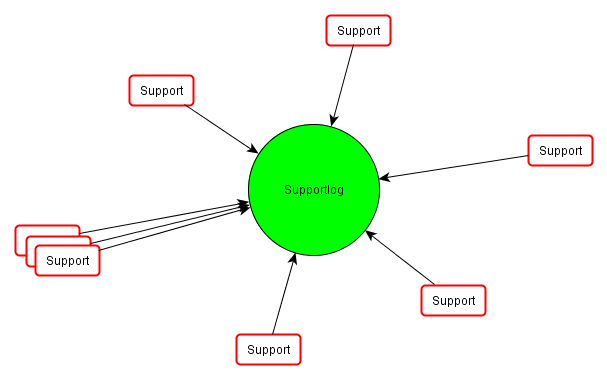
\includegraphics[width=10cm]{kapitel/gruppe3/bilder/grafik_supportlog}
	\caption{Unabhängige Supportleister dokumentieren in zentralem Log}
	\label{fig_zentraler_supportlog}
\end{figure}

Es ist dabei unerheblich, ob die Supportleister die Unterstützung als Kern ihrer Aufgabe leisten, oder ob es sich um kollegiale Unterstützung bei einem Problem handelt. Gerade letztere Information aufzufangen ist wichtig, da diese sonst nur eine sehr schwer einzuschätzende Größe bleibt.

Dieser Dokumentationsoverhead ist gering gegenüber dem Overhead eines stark reglementierten Supportsystems, erhält alle Vorteile unbürokratischer, schneller Hilfeleistung und fängt zusätzlich Informationen über Art und Umfang gelisteten Supports auf.

\subsubsection{Knowledge Base}
Aus dem Supportlog kann eine durchsuchbare Knowledge Base aufgebaut werden, die nicht nur die allgemeinen Fehlerquellen und Schwierigkeiten von Software im Einsatz beleuchtet, sondern ganz speziell die an der Hochschule in dieser Zusammenstellung einmalige Konfiguration.
Dadurch kann sehr viel schneller auf spezifische Fehlerszenarien reagiert werden, als dies mit allgemeinen Informationen möglich ist.

Auch können aus dem Supportlog FAQs abgeleitet werden, die tatsächlich dem Wortsinn nach Listen häufig gestellter Fragen und Antworten darstellen, und nicht was mehr oder minder begründet vermutet wird.

Auch zeigt sich in den Häufigkeiten bestimmter Probleme, wo spezielle Dokumentation und Hilfetexte notwendig sind, die ebenfalls hinterlegt werden können.

Hierzu muss das Supportlog allerdings von einer geeigneten Stelle regelmäßig gesichtet werden.

\subsection{Fortentwicklung}
Eine Konzeption kann nur aktuelle Trends und Entwicklungen berücksichtigen. Es ist schwierig vorauszuschauen, was die Zukunft danach bringen wird, welche Trends mehr oder weniger wichtig sind, und welche Trends darauf folgen werden.

Allerdings ist es keine Frage, dass eine Hochschule länger Bestand hat, und es damit sinnvoll ist, Prozesse zu hinterlegen, die neue Trends und Entwicklungen zwar nicht vorwegnehmen, aber deren zeitnahe Entdeckung und Integration ermöglichen.

Auch zeigt sich in der Praxis, dass unvorhergesehene Bedingungen und Ereignisse theoretisch gut ausgearbeitete Prozesse übermäßig blockieren, und eine Anpassung geschehen muss.

\subsubsection{Feedback}
Hierzu muss an jedem Punkt des Gesamtsystems dem Benutzer möglich sein, Feedback zu geben. Mehr noch muss gerade bei neuen oder überarbeiteten Prozessen dieses Feedback eingefordert werden, um die Qualität des neuen Prozesses oder Tools einschätzen zu können.

Das Feedback gelangt an die zuständige Stelle, muss aber auch zentral gesammelt werden, ähnlich wie das Supportlog. Diese Sammlung wird zentral ausgewertet, um verdeckte, verteilte Probleme aufzudecken, die sich in Feedback an unterschiedliche Stellen verbergen können.

Auf die Auswertung muss wo sich Probleme zeigen, eine Information der zuständigen Stelle folgen, damit eine Verbesserung erarbeitet werden kann. Entsprechend ist die zuständige Stelle berechtigt, ein Meeting einzuberufen, damit ihre Eingaben nicht einfach verloren gehen können, sondern zwangsläufig mindestens einmal besprochen werden.

\subsubsection{Innovationseingabe}
In den Feedbackprozess eingebettet muss die Möglichkeit für jede Person sein, Innovationen aus beliebiger Quelle zu beschreiben, so dass Entwicklungen nicht erst von bestimmter Stelle wahrgenommen werden müssen, um erwägt zu werden. Damit kann von beliebiger Stelle aus eine Verbesserung zur Diskussion gebracht werden.

Damit diese Möglichkeit von Benutzern angenommen wird, muss auf Eingaben angemessen schnell reagiert werden. Um eine ernsthafte Reaktion zu gewährleisten, müssen diese Vorschläge auch diskutiert worden sein.

\subsubsection{Erfahrungsgetriebene Fortentwicklung}
Aus den Erkenntnissen über Schwachstellen aus dem Supportlog, den Benutzerberichten und -bewertungen aus dem Feedbacklog und den Innovationseingaben können nicht nur Schwachstellen und Fehler in Prozessen identifiziert werden, sondern auch Trends in der Benutzung des Systems erkannt. Da Support und Feedback andauernde Prozesse sind, ergibt sich daraus ein selbstregulierendes System, das, wenn die Messgrößen Supportlog und Feedbacklog angemessen berücksichtigt werden, evolutionär verbessert.

\begin{figure}[h!]
	\centering
	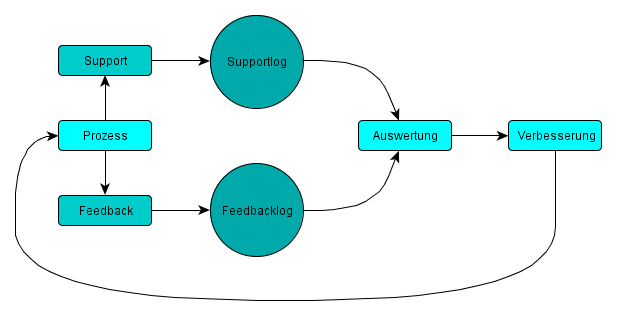
\includegraphics[width=10cm]{kapitel/gruppe3/bilder/zyklus_prozessverbesserung}
	\caption{Zyklus der Verbesserung eines Prozesses}
	\label{fig_zyklus_prozessverbesserung}
\end{figure}






















\section{Hard- und Software}
Zur Integration eines hochschulweiten Informationsmanagements können bezüglich der IT mehrere Ansätze gefahren werden.

Zum einen kann eine ganzheitliche integrierte Lösung verwendet werden. Die Universität Hamburg hat einen vollständigen Neuanfang bezüglich der Campussoftware gewagt mit der integrierten Gesamtlösung „CampusNet“ der Datenlotsen Informationssysteme GmbH. Dies resultierte aus der Zusammenlegung mehrerer Fachbereiche zu einzelnen Fakultäten. Die verschiedenen Teillösungen waren größtenteils inkompatibel oder aufgrund von Eigenentwicklung schwer wartbar.\footnote{\cite{dini_webportale_2007}}

Laut Günter Müller, Leiter des Rechenzentrums, existieren an der Hochschule Emden Leer derart verschiedene Teillösungen nicht. Auch würden sich Eigenentwicklungen auf vernachlässigbare Systeme beschränken. Software würde grundsätzlich für die gesamte Hochschule eingesetzt.\footnote{Interview}

Der Einsatz einer integrierten Gesamtlösung zur Beseitigung von Inkompatibilitäten und schwer wartbaren Eigenentwicklungen kann somit keine Argumentationsgrundlage sein.
Des Weiteren reicht die bisherige Analyse nicht aus, um einen vollständigen Anforderungskatalog zu bilden, auf dessen Grundlage eine integrierte Gesamtlösung gefunden werden kann.

Stattdessen wird auf eine flexible Lösung gesetzt, welche den Einsatz einzelner Fachanwendungen zur Lösung bestimmter Probleme vorsieht. Personelle und finanzielle Ressourcen sind dadurch flexibler einsetzbar, auf veränderte Anforderungen an eine Lösung kann flexibler reagiert werden und die Abhängigkeit von einem Anbieter für alle Anwendungen wird aufgelöst.

\subsection{Kernanforderungen}
Bei Core-Systemen wird weiterhin auf Appliance Lösungen gesetzt. Das minimiert Fehlerpotenzial und den operativen Betrieb.\footnote{Interview}

Softwaresysteme laufen auf virtuellen Maschinen. Die bessere Hardwareauslastung und Möglichkeit der automatisierten Administration kann finanzielle und personelle Ressourcen sparen.\footnote{\cite{baun_servervirtualisierung_2009}}

Die Systeme sind weniger abhängig von der Hardware, was dessen Austausch erleichtert. Netzwerkanbindung, Rechenleistung und Speicherkapazität sind somit flexibler an sich verändernde Anforderungen anpassbar.

Die eingesetzte Software soll in die Systemlandschaft integrierbar, lösungsorientiert und möglichst barrierefrei, sowie systemunabhängig sein. Dies unterstützt auch den Ansatz der Freiheit in Forschung und Lehre.

Die Systemunabhängigkeit kann durch Webanwendungen im Sinne des Ansatzes Software as a Service (SaaS) erreicht werden. Um möglichst alle gängigen Browser und Endgeräte zu unterstützen, sollten die Anwendungen den Standards des World Wide Web Consortiums (W3C) gerecht werden und sofern möglich dem Ansatz responsive design gerecht werden. Dadurch kann auch dem Trend bring your own device Rechnung getragen werden.

\subsection{Bereichsübergreifende Basissystem}
In den Bereichen Forschung, Lehre und Verwaltung fallen informationstechnologische Aufgaben an, für die eine zentrale IT-gestützte Lösung geschaffen werden kann. Das verringert redundante Daten und Systeme sowie administrative Aufwände. Im folgenden werden Lösungen für einzelne Aspekte des Informationsmanagements aus IT-Sicht vorgestellt, die in allen drei Bereichen genutzt werden können. Weiterhin dienen sie teilweise als Grundlage für spezialisierte Systeme.

\subsection{Identity Management}
Um die Anzahl an verschiedenen Accounts zu minimieren, sollten die Benutzer zentral gepflegt werden. Dies kann in einem Verzeichnisdienst wie dem bereits eingeführten Active Directory geschehen. Die Authentifizierung an einem System findet dann nicht am System selbst statt, sondern mit Hilfe des Verzeichnisdienstes. Der Anwender muss sich nur einen Account zzgl. Kennwort merken, um sich an verschiedenen Systemen anzumelden. Weiterhin gilt eine Aktualisierung von Informationen global, wodurch Inkonsistenzen aufgelöst werden.

Zuzüglich zum zentralen Verzeichnisdienst ist auch ein SingleSignOn (SSO) Mechanismus empfehlenswert\footnote{\cite{zahn_itmanagement}}, wie es an der Universität Augsburg durch das System Webauth umgesetzt ist.

Für das Lernraumsystem moodle gibt es bereits ein SSO Plugin.\footnote{\url{http://sourceforge.net/projects/moodleldapsso}}

Alle weiteren Websysteme sollen auf SSO umgestellt werden, um dem Benutzer eine möglichst integrierte Landschaft zu bieten. Weiterhin sollte jedes System aus Sicherheitsgründen insofern angepasst werden, dass auch ein SingleSignOff möglich ist. Die zentrale Abmeldung soll gewährleisten, dass die Benutzenden auf allen Systemen, auf denen sie sich bewegt haben, abgemeldet sind.

Die Benutzerdatenpflege sollte auf den einzelnen Systemen ausgeschaltet sein und ausschließlich über ein zentrales Formular geschehen. So wird ein konsistenter Datenbestand gesichert. Insofern die Informationen in anderen Systemen benötigt werden, müssen diese vom zentralen System automatisiert und über gesicherte Verbindungen verteilt werden. Ein weiterer Vorteil ist, dass die Informationen, da zentral gesammelt, auch zentral ausgewertet werden können.

So ist es möglich diese zentralen persönlichen Informationen mit Informationen anderer Art aus anderen Systemen anzureichern und weiterzuverwenden. So können automatisierte Reports über Forschungsprojekte erstellt werden, Expertisen zu bestimmten Themen identifiziert werden oder für die Verwaltung Verknüpfungen von Personen zu verwaltungstechnischen Aufgaben. Die Umsetzung ist dabei individuell an die Gegebenheiten und Informationsbedarfe der Hochschule anzupassen.\footnote{\cite{vogl_fortschritte_2012}} Dementsprechend wird die technische Lösung eine Individuallösung werden.

\subsection{Geschäftsprozesse}
Neben der Forschung gibt es an Hochschulen gerade im Verwaltungsbereich viele Geschäftsprozesse, die in der Regel immer gleich ablaufen. Problem ist, dass Personen unterschiedlichster Bereiche involviert sind und die Prozesse nicht ausreichend definiert sind.\footnote{\cite{becker_prozesse_2010}}

Die Modellierung der Prozesse sollte im ersten Schritt auf abstraktem Niveau stattfinden. Dies erleichtert den Einstieg und macht Verbesserungspotenziale sichtbarer. In der WWU Münster wurde dafür die PICTURE Methode verwendet.
Im zweiten Schritt kann der ggf. angepasste Prozess konkretisiert und in Form des Industriestandards Business Process Model Notation (BPMN) festgehalten werden. Ein Client-Tool zur Erstellung von BPMN ist das Activiti BPMN 2.0 Eclipse Plugin.\footnote{\url{http://docs.codehaus.org/display/ACT/Activiti+BPMN+2.0+Eclipse+Plugin}}

Mit Hilfe der zentralen Business Process Management (BPM) Platform activiti können die Prozesse aktiv den Workflow verbessern, Konsistenz wahren und zeitliche Ressourcen sparen.  Die Plattform ermöglicht REST Anfragen, wodurch die Prozessinformationen auch in andere Applikation integriert werden können. Der Activiti Explorer ermöglicht den voll funktionalen Zugriff via Weboberfläche. Somit wird der Kernanforderungen SaaS Rechnung getragen. Weiterhin ist Activiti Open Source und somit ausbau- und anpassungsfähig.\footnote{\url{http://activiti.org/index.html}}

Durch activiti wird es möglich sein die Automatisierung von einzelnen Prozessen Stück für Stück voranzutreiben. Einzelne Teile des Workflows können automatisiert Scripte starten, E-Mails verschicken und ähnliches und somit stückweise die manuelle Bearbeitung reduzieren. Außerdem können Serviceanfragen damit zentralisiert verwaltet werden. Durch Definition von Feldern für einzelne Prozessschritte können vorab benötigte Informationen festgelegt werden, sodass Nachfragen vermieden werden.

\subsection{Content Management}
Um den wachsenden Anforderungen in Bezug auf Content Management genüge zu tun wurde an der WWU Münster das Enterprise Content Management System alfresco eingeführt. Auch an einer kleinen Hochschule kann ein solches System eingesetzt werden. Alfresco bietet diverse Vorteile. Die für dieses Konzept Relevanten werden hier kurz aufgelistet:\footnote{\cite{kloetgen_2012}}

\begin{itemize}
	\item Unterstützung für mobile Endgeräte
	\item Anpassungs- und ausbaufähig
	\item diverse Zugriffsmöglichkeiten zur Nutzung innerhalb bekannter Standardanwendungen
	\item Publikation in sozialen Netzwerken
	\item Unterstützung verschiedener Standardschnittstellen
	\item Activiti Workflow Engine
	\item Metadaten
\end{itemize}

Alfresco bietet damit die ideale Grundlage verschiedene Informationen zu verwalten sowie die Unterstützung des vollständigen Dokumenten-Lifecycles - von der Erstellung über die Bereitstellung bis zur Archivierung. 

Die Anbindung der Dokumente ist dynamisch und durch die zahlreichen Standards ideal integrierbar. So kann ein an verschiedenen Orten auf verschiedene Arten bereitgestelltes Dokument an einer Stelle aktualisiert werden wodurch an allen Zugriffsstellen die aktuellste Version bereitgestellt wird.

Dennoch ist das System flexibel genug auch bestimmte Versionen eines Dokuments bereitzustellen. Dank der integrierten Versionierung entfällt außerdem der aufwendige Wiederherstellungsprozess. Dank der Möglichkeit Metadaten anzugeben, wird der Weg für eine brauchbare Dokumentensuche geebnet.

\subsection{Spezialsysteme}
Unter Spezialsystemen sind hier Softwarelösungen zu verstehen, die bei speziellen Aufgaben im Hochschulalltag unterstützen sollen.

\subsection{Verwaltungssoftware}
Software, die speziell in der Verwaltung genutzt wird, ist in dieser Ausarbeitung ausgenommen, da die Anforderungen sehr speziell sein können und die Wissensbasis innerhalb dieser Ausarbeitung nicht ausreicht, um eine Empfehlung zu geben.

Erwähnt werden sollte dennoch, dass die Universität Karlsruhe erfolgreich Schnittstellen zu den HIS-Systemen integriert hat.\footnote{\cite{dini_webportale_2007}}

Da dieses Konzept auf einem ähnlich flexiblen Ansatz basiert, besteht die Möglichkeit, dass auch Verwaltungssoftware integriert werden kann, wenn sie die genannten Kernanforderungen erfüllt.

\subsection{Lernplattform}
Die Hochschule setzt bereits erfolgreich und in vielen Bereichen das System moodle ein. Die Nutzung der Funktionen variiert dabei zwischen den einzelnen Fachbereichen.
Solange moodle die Anforderungen der Hochschule an eine Lernplattform erfüllt, besteht kein Grund das System auszutauschen.

Neben den bereits genutzten Standardfunktionen ist moodle ausbaufähig.
Beim Aufruf von moodle soll die Authentifizierung durch einen SSO Mechanismus geschehen. Hat sich ein Benutzer bereits an einem anderen System authentifiziert, ist dieser beim Aufruf sofort angemeldet. Integriert werden sollte auch der SingleSignOff Mechanismus.
Statt der Stammdatenänderung via moodle wird auf ein zentrales Formular weitergeleitet, um persönliche Informationen zentral und damit konsistent zu halten.

Die in den Kursen zur Verfügung gestellten Dateien jeglicher Art werden in alfresco gepflegt und von moodle angebunden. Die entsprechenden Schnittstellen und Plugins müssen nicht neu entwickelt werden.

Vorteil ist, dass die Dokumente in alfresco verwaltet werden. In moodle kann dann eine bestimmte Version oder die jeweils aktuellste referenziert werden. Bei den Dokumenten kann es sich um Textdokumente, Audio oder auch Videofiles handeln. Durch alfrescos Unterstützung für mobile Endgeräte wird so den Zugreifenden auch die Möglichkeit gegeben ein Dokument auf den verschiedensten Endgeräten anzuzeigen.

Dank alfresco können Dokumente nicht nur innerhalb moodle via Weboberfläche aufgerufen werden, sondern auch bequem via Filesystem. Eine Datei kann somit auf verschiedene Art und Weise abgerufen werden – je nach dem welchen Weg der Anwender für den aktuell praktikabelsten hält.

\subsection{Publikationen}
Um Wissenschaftler bei der Publikation von Zeitschriften zu unterstützen setzt die WWU Münster auf die Plattform Open Journal System (OJS). Es bietet die Möglichkeit elektronische Zeitschriften zu verwalten und den gesamten Publikationsworkflow abzubilden.\footnote{\cite{kloetgen_2012}}

Grundsätzlich sollte auch ein Workflow in activiti implementiert werden, der bei der Publikation unterstützt. So können wichtige Metadaten aufgenommen und an relevante Systeme weitergegeben werden. Ändern sich Systeme oder kommen neue hinzu, müssen sich Wissenschaftler nicht umgewöhnen, sondern nutzen weiterhin den in activiti hinterlegten, für die neuen Systeme jedoch angepassten, Prozess. Dadurch besteht auch die Möglichkeit ein publiziertes Dokument zusätzlich in alfresco abzulegen, wenn ein Anwendungsfall dies benötigt.
OJS bietet die Möglichkeit der Authentifizierung via Single Sign On. Dies geschieht via Shibboleth.\footnote{\url{https://pkp.sfu.ca/wiki/index.php?title=Setting_up_authentication}}

Neben der Konfiguration von Single Sign On sollte auch hier den Benutzenden die Möglichkeit des Single Sign Off gegeben werden.

\subsection{Evaluation}
Wie auch die Universität Münster\footnote{\url{https://www.wiwi.uni-muenster.de/fakultaet/de/studium/lehrevaluation}} und die TU Dortmund\footnote{\url{https://www.itmc.uni-dortmund.de/dienste/e-learning/umfragewerkzeuge.html}} setzt die Hochschule Emden Leer bereits die Software EvaSys zu Evaluationszwecken ein. Sie ist webbasiert und entspricht damit dem Software as a Service Gedanken.
Seit Version 5 unterstützt EvaSys auch die SingleSignOn Authentifizierung\footnote{\url{http://www.ku.de/fileadmin/190304/Feature_Function_Benefit_EvaSys_V5.0_DE.pdf}}, welche auch an der Hochschule Emden Leer eingesetzt werden soll.

\subsection{Campus Portal}
Ein Campus Portal dient als zentrale Anlaufstelle für alle Hochschulangehörigen und ist ein personalisiertes Webportal. Es soll die Verwaltung persönlicher Daten ermöglichen, eine Übersicht über informationstechnische Funktionen inklusive Weiterleitung zum entsprechenden System integrieren, sowie aktuell relevante Informationen in Form einer Agenda anzeigen.

Unter den informationstechnischen Funktionen sind alle Werkzeuge und Systeme zu verstehen, die einem bestimmten Zweck dienen. Eine Selbstimplementierung für die bereitzustellenden Funktionen soll dabei vermieden werden.

Stattdessen soll, wie in den Kernanforderungen aufgenommen, auf existierende Systeme gesetzt werden, sofern dies möglich ist. Beim Campus Portal werden die Kernanforderungen an diese Systeme, nämlich integrierbar und systemabhängig (SaaS) zu sein, nun deutlich.

Ein solches Campus Portal ist vor allem der Informationsübersicht dienlich. Durch personalisierte und dynamisch generierte Inhalte gewinnen die Benutzenden einen Überblick über die Informationen, die sonst in verschiedenen Systemen verteilt sind. Die Integration der Systeme kann schrittweise erfolgen, sollte jedoch zur Akzeptanzgewinnung bei Veröffentlichung eine gewisse Menge externer Systeme integrieren.

Die Universität Karlsruhe hat im ersten Schritt das Veranstaltungsmanagement und die Prüfungsverwaltung der Software-Systeme der HIS GmbH in das Portal integriert.

Orientiert am Anforderungskatalog der WWU Münster an ein solches Portal1 und unter der Voraussetzung, dass die in diesem Konzept genannten Systeme umgesetzt werden, kann ein zukünftiges CampusPortal folgende Informationen konsolidieren:

\begin{itemize}
	\item Kalender
	\begin{itemize}
		\item Abonnement-Prinzip
		\item Detailinformationen, zum Beispiel Kontoinformationen für Rückmeldegebühren
		\item Agenda aus moodle
	\end{itemize}
	\item Referenz zu gewählten Kursen (moodle)
	\item Referenz zum E-Mail-Portal (Outlook Web App)
	\item Suchmaschine
	\item offene Tasks im BPM System
	\item Start möglicher Tasks im BPM System (zum Beispiel Workflow für die Publikation)
	\item offene Evaluationen
\end{itemize}

Unter der Voraussetzung, dass auch andere Hochschulsysteme integrierbar sind, können folgende Punkte aus dem Anforderungskatalog der WWU Münster zusätzlich im Campus Portal integriert werden:

\begin{itemize}
	\item Stundenplan
	\item Vorlesungsverzeichnis inkl. Details
	\item Leistungsübersicht
	\item Hochschulleben
	\begin{itemize}
		\item Mensapläne
		\item Hochschulsport
		\item Veranstaltungen
	\end{itemize}
	\item Einführung
\end{itemize}

Alternativ dazu kann auch das Konzept eines Hilfesystems integriert werden, das via Sprechblasen Hilfestellungen oder Informationen anzeigt zur Funktion auf der sich der Mauszeiger gerade befindet.

Die technische Struktur kann analog zu der des Portals myWWU der Universität Münster aufgebaut sein.
\begin{figure}[h!]
	\centering
	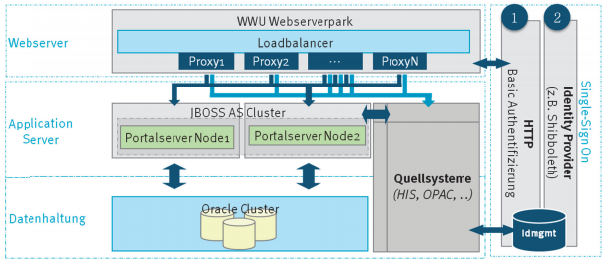
\includegraphics[width=10cm]{kapitel/gruppe3/bilder/struktur_mywwu}
	\caption{technische Struktur des Portals myWWU der Universität Münster}
	\label{fig_struktur_mywwu}
\end{figure}

\subsubsection{Integrierte Gesamtsuche}
Wissenschaftliche Informationen sind häufig in verschiedenen Systemen angesiedelt. Durch die Einführung eines Systems zur integrierten Gesamtsuche wird die Suche an zentraler Stelle ausgeführt. Einzelne Systeme werden beim Suchen nicht vergessen. Die Integration neuer Systeme erleichtert die Kommunikation derer Integration in das wissenschaftliche Umfeld.

Die WWU Münster nutzt dafür einen „Suchmaschinen-basierte[n] Ansatz auf Basis der Software Primo von der Firma Ex Libris“.\footnote{\cite{vogl_fortschritte_2012}} Dafür nötig ist eine Normalisierung der Datenformate interner und externer Quellen, welche „insbesondere auf der Detailebene […] aufwändige Anpassungen und Eigenentwicklungen notwendig“ machen.

Quellsysteme ausgehend von diesem Konzept können sein:
\begin{itemize}
	\item alfresco
	\item Identity Management System
	\item ForschungsDB Niedersachsen
	\item moodle
	\item Open Journal System
	\item Hochschulexterne Informationssysteme wie zum Beispiel video2brain
	\item ggf. Bibliothekssuche
\end{itemize}

Wichtig ist neben korrekten und vollständigen Ergebnissen auch die Benutzbarkeit. Bekannte Funktionalitäten aus anderen Suchmaschinen, wie Gruppierungen, sollten integriert sein, wie auch eine übersichtliche und funktionale Benutzeroberfläche.

\subsection{Ausblick bei Integration der Bibliothek}
Die Best Practices zeigen, dass auch die Bibliotheken der Hochschulen und Universitäten bei Informationsmanagement-Projekten integriert werden. Die dort vorhandenen Informationen werden vor allem für Forschung und Lehre genutzt, welches die Kernaufgaben von Hochschulen sind.

Neben der Anbindung der Bibliothekssuche in die integrierte Gesamtsuche kann auch ein Digitalisierungssystem für archivierte Zeitschriften und Bücher zur Aufwertung der gesuchten Informationen beitragen. Die WWU Münster setzt dafür das vor Ort frei verfügbare Scanner zuzüglich der Software scantoweb ein.




\section{Abwägung des Einsatzes eines Informationsmanagements an der Hochschule Emden Leer}
Das Soll-Konzept analysiert die Ist-Situation um festzustellen, ob es generell einer Verbesserung des Informationsmanagements bedarf und wo diese anzusetzen sind oder ob noch kein Informationsmanagement besteht und aufgebaut werden muss. Dazu sind verschiedene Aspekte zu beleuchten. Neben der Anforderung des Marketings und neben den  technischen Neuerungen und Umsetzungen ist zu klären, wer die strategische und operative Führung übernehmen soll. 

Im klassischen Informationsmanagement ist dies die Aufgabe eines Chief Information Officers. Der Informationsmanager dient dabei als zentrale Schnittstelle zwischen technischen, organisatorischen und wirtschaftlichen Teilbereichen und dient dort als sogenannter Mittler und untersucht dafür die Informations- und Kommunikationstechniken in allen unterschiedlichen Bereichen um diese sinnvoll einzusetzen.\footnote{\cite[86]{krcmar_einfuhrung_2015}}

\begin{figure}[h!]
	\centering
	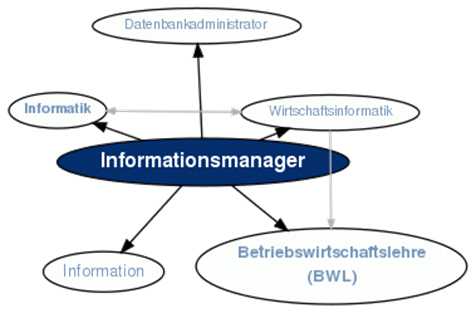
\includegraphics[width=10cm]{kapitel/gruppe3/bilder/definition_informationsmanager}
	\caption{Definition Informationsmanager}
	\label{fig_definition_informationsmanager}
\end{figure}

\subsection{Analyse des Ist-Zustandes}
Bezug nehmend auf die Abbildung \ref{fig_organigramm_HS} und der festgestellten Ist-Analyse ist festzuhalten, dass der Hochschule Emden kein Informationsmanagement im klassischen Sinne zugrunde liegt, sondern ein zentrales Informationssystem.

Es werden verschiedene Dienste und Möglichkeiten wie Moodle, Eduroam zur Verfügung gestellt und in Anspruch genommen.

Es gibt keine Verwaltung, sondern verschiedene Bereiche, die unterteilt sind in Arbeitsgruppen, Abteilungen sowie Rechenstelle und Pressestelle.

Weiterhin beinhaltet das Informationssystem verschiedene Prozesse zum Datenaustausch, bzw. Datenfluss und Backuptransfer  aus verschiedenen Systemen.\footnote{Ist-Situation \#8}

Die Nutzung des gegenwärtigen Informationssystems wird unterschiedlich stark genutzt oder ausgelastet.

Von den zentralen Einrichtungen nehmen das Hochschulrechenzentrum und die Bibliothek einen wichtigen Platz in der Hochschule ein. Das Hochschulrechenzentrum übernimmt derweil viele Aufgaben der Informationsverwaltung und Planung.

Doch nicht nur da werden Informationen gesammelt und  ausgewertet. Die Hochschule in Emden definiert eine ganze Reihe von Arbeitsgruppen, beispielsweise die Arbeitsgruppe Zahlen, Daten, Fakten, die Kennzahlen der Hochschule und der einzelnen Fachbereiche sammelt und diese auswertet.\footnote{Ist-Situation \#8}

Aktuell besteht keine Vernetzung verschiedener Intranetzsysteme zwischen verschiedenen Hochschulen.

\subsection{Analyse des zu erwartenden Soll-Zustandes}
Nach Betrachtung der Best-Practice Beispiele anderer Hochschulen, lässt sich erkennen, dass jede Hochschule und auch Universität den Umgang des Informationsmanagements anders angeht. So spielen verschiedene Faktoren eine Rolle, die an jeder Hochschule unterschiedlich ausgelegt sind.

Ein Vergleich der betrachteten Hochschulen mit der Hochschule Emden zeigt, dass Emden eine wesentlich kleinere Hochschule ist und somit andere Ansprüche sowie nicht so komplexe Strukturen besitzt, als beispielsweise die WWW Münster, die über 40.000 Studierende pflegt.

Trotz unterschiedlich integrierter Möglichkeiten zur Umsetzung des jeweiligen Informationsmanagements, gibt es doch Bereiche die gleich oder relativ ähnlich sind. So sind Bibliotheken, Gremien, Ausschüsse, ebenso wie Fachbereiche und auch das Präsidium Teil einer jeden Hochschule oder Universität.

Es ist zu schauen wo sich das Informationsmanagement ansetzen lässt um mehrere Bereiche und Bestandteile untereinander zu verbinden. Fakt ist, dass es in Emden bereits Arbeitsgruppen gibt, die bestimmte Informationen gewinnen und filtern. So wäre der Aufbau einer neuen Struktur eine Möglichkeit zur Verbesserung des Informationsaustausches.

\subsection{Soll-Möglichkeit}
\subsection{Zu erwartende Kosten}
\subsection{Prognose und zu erwartender Verlauf / Fazit}
%\chapter{Konzept zur Erreichung der Soll-Situation}

Autoren: Marco Beckmann, Christian Halfmann

Ich bin ein Einleitungstext, der noch geschrieben werden muss.

\section{Umsetzungsplanung}
Ich bin ein einleitender Text, der noch geschrieben werden muss.

\subsection{Positionsbestimmung}
Für einen erfolgreichen Umsetzungsplan mit der Zielsetzung einer Neuordnung des Informationsmanagements an einer Hochschule ist eine Positionsbestimmung der aktuellen Situation von elementarer Bedeutung. Hierzu muss der Ist-Zustand des aktuellen Informationsmanagements mit der Zielformulierung des avisierten Informationsmanagements an der Hochschule erfasst und abgeglichen werden. 

Da solche Veränderungen in der Regel einen langwierigen Prozess darstellen, ist es ratsam, Prioritäten zu definieren und die einzelnen Teilbereiche anhand der Dringlichkeit umzusetzen.

Ist die Position bestimmt, kann davon ausgehend ein entsprechender Migrationsplan (vgl. Kapitel \ref{section_migrationskonzepte}) und, wenn noch nicht geschehen, ein Changeplan (vgl. Kapitel \ref{subsection_change_management}) erstellt werden. Je nach Art und Umfang der Veränderungen sollte allerdings das Change Management nicht erst nach der Positionsbestimmung angewandt werden, sondern schon bei der Zielbestimmung – also mit in die Erarbeitung des möglichen Soll-Zustands einfliessen.

Diese Ausarbeitung wird sich aus Gründen der Komplexität im praxisbezogenen Teil nicht auf das gesamte Informationsmanagement der Hochschule Emden/Leer beziehen können. Exemplarisch wird daher eine Umsetzungsplanung an den Beispielen des Dokumentenmanagements Alfresco und der Erstellung eines responsive Designs der Webpräsenz der Hochschule erarbeitet.

Alfresco wird derzeit noch nicht an der Hochschule eingesetzt. Zur Zeit werden Dokumente in verschieden Systemen verwaltet und zugäglich gemacht. Für die Webpräsenz wird derzeit ein TYPO3-System in der Version 4.5 LTS (Long Term Support) genutzt, welches noch nicht für mobile Endgeräte optimiert ist.

\subsection{Change Management}
\label{subsection_change_management}

Ich bin ein einleitender Text, der noch geschrieben werden muss.

\subsubsection{Grundlagen des Change Managements}
Die Umsetzung einer Neuordnung des Informationsmanagements an einer Hochschule bedeutet auch Wandel und Veränderungen. Um das optimal zu steuern, bedarf es spezieller Managementtechniken, welche sich unter dem Begriff Change Management zusammenfassen lassen. Im Vordergrund aller Betrachtungen steht der Faktor Mensch, denn für eine erfolgreiche Umsetzung von Veränderungen ist die aktive Unterstützung der Betroffenen von erheblicher Bedeutung.\footnote{\cite{lauer_change_2014}}

Nach Thomas Lauer sollte das Change Management grundsätzlich an drei Punkten ansetzen:
\begin{itemize}
	\item Individuum: Das Individuum beschreibt jeden Einzelnen. Ohne die Mitarbeit der Betroffenen ist ein Wandel unmöglich. Das Change Management soll nicht nur die Fähigkeiten des Einzelnen an neue Herausforderungen anpassen, sondern auch die positive Einstellung gegenüber der Ziele des Wandels aller Betroffenen fördern.
	\item Unternehmensstruktur (bzw. Hochschulstruktur): Die Unternehmensstruktur umfasst Aufbau- und Ablauforganisation sowie Strategien und Ressourcen. Veränderungen in diesen Bereichen sind auf dem Papier grundsätzlich einfach.
	\item Unternehmenskultur (bzw. Hochschulkultur): Die Unternehmenskultur beschreibt dauerhafte, über lange Zeit gewachsene Strukturen die für Einstellung, Werte und Regeln des Umgangs verantwortlich sind. 
\end{itemize}

In den meisten Fällen bringt ein Wandel in den oben genannten Bereichen Veränderungen in allen Dimensionen mit sich, die sich wechselseitig beeinflussen.\footnote{\cite{fisch_veraenderungen_2008}} 

So ist z. B. ein Wandel ohne die Einbeziehung der Unternehmenskultur oftmals zum scheitern verurteilt.\footnote{\cite{lauer_change_2014}} Das heißt, für ein erfolgreiches Change Management sollten grundsätzlich die Abhängigkeiten der Bereiche untereinander berücksichtigt werden.

Veränderungen bedeuten Neues und Ungewohntes für alle Betroffenen. 
Betroffene müssen veränderte Aufgaben erledigen, neue Technologien und Methoden erlernen, erneut soziale Beziehungen zu Kollegen, Vorgesetzten oder Kunden aufbauen, mit Problemen in der Implementierungsphase umgehen und ggf. ihre Werte in Einklang mit neuen Standards und Zielen der Organisation bringen.\footnote{\cite{fisch_veraenderungen_2008}}

Dies kann zu Zweifeln und Widerständen führen, was im schlimmsten Fall ein Scheitern des gesamten Vorhabens bedeuten kann. Als Ursache eines gescheiterten Wandels steht der Widerstand an oberster Stelle. Mangelhafte Prozessteuerung, zu schnelles Veränderungstempo und unklare Zielsetzungen spielen dabei ein wichtige Rolle und können Gründe für eben diesen Widerstand sein.\footnote{\cite{lauer_change_2014}}

Die Bereitschaft zum Wandel nimmt zu, wenn die Betroffenen überzeugt sind, das die Veränderungen ihnen persönlich nutzen, ihre Identität nicht bedroht ist und ihre Werte und Ziele mit dem Wandel in Einklang gebracht werden können.

Des weiteren wird die Bereitschaft zum Wandel gefördert wenn die Betroffenen über Fähigkeiten verfügen, die den veränderten Anforderungen gerecht werden. Die Aufgabe des Change Management ist es, durch Information, Partizipation, Unterstützung (z. B. Coaching) und Anreizgestaltung den Betroffenen die Zweifel und Unsicherheit zu nehmen.\footnote{\cite{fisch_veraenderungen_2008}} 

\begin{itemize}
\item \textbf{Kommunikation}
Nach Thomas Lauer ist einer der entscheidendsten Erfolgsfaktoren des Change Managements die Kommunikation. Kommunikation schafft Transparenz und damit Orientierung und dient damit auch der Beilegung von Widerständen. Damit ist aber auch ein potenzieller Misserfolg eines Change Managements auf die Kommunikation zurückzuführen. Fehlinterpretationen und Missverständnisse können schnell zu Konflikten führen.\footnote{\cite{lauer_change_2014}}

Es sollten also entsprechende Kommunikationsstrategien und Kommunikationspläne erarbeitet werden, um die Betroffenen für die Veränderungen zu gewinnen und Missverständnissen aus dem Weg zu gehen. In der Startphase sollten die Betroffenen über Gründe, Ziele, Notwendigkeit, Nutzen und den zeitlichen Ablauf informiert werden. Aber auch potentielle Risiken und Schwierigkeiten sollten von Anfang an offen kommuniziert werden.\footnote{\cite{fisch_veraenderungen_2008}}

In der Durchführungsphase ist es wichtig die Kommunikation aufrecht zu erhalten. Beispielsweise können Projektfortschritte regelmäßig an alle Betroffenen weitergegeben werden. Durch das Aufrechterhalten der Kommunikation können frühzeitig Widerstände erkannt und überwunden werden.\footnote{\cite{lauer_change_2014}} 

\item \textbf{Partizipation}
Ein weiterer wichtiger Erfolgsfaktor ist die Partizipation. Das Einbinden möglichst vieler Betroffenen in den Change Prozess erhöht die Motivation und hilft den Betroffenen sich mit den Veränderungen zu identifizieren. Haben Betroffene andere Positionen oder Sichtweisen gegenüber des Wandels als die Organisation müssen diese Widerstände nicht gleich negativ ausgelegt werden. Die Ideen und Vorschläge der Betroffenen können in den Change Prozess einfliessen und weiterhin Veränderungen optimieren.

\item \textbf{Unterstützung}:
Besonders wenn es um neue Technologien, Werkzeuge oder Verfahren geht, ist Unterstützung für die Betroffenen gefordert. Die Unterstützung hat zum Ziel, die Betroffenen des Wandels auf die zusätzlichen oder neuen Anforderungen vorzubereiten. In den Meisten Fällen geschieht das in Form von Weiterbildung oder Coaching.

Des weiteren fördert eine vom Unternehmen ausgehende Weiterbildung nicht nur den Aufbau von Qualifikationen und die Erweiterung des Wissens der Betroffenen, sondern auch die Motivation. Den Betroffenen wird das Gefühl gegeben, dass in sie investiert wird und damit auf eine langfristige Partnerschaft gesetzt wird.
\end{itemize}

In dem Sinne ist die Aufgabe des Change Managements also nicht die Definition von Zielen, es soll den Weg des gesamten Vorhabens vom Ausgangspunkt bis zum Ziel gestalten\footnote{\cite{lauer_change_2014}} und den Betroffenen des Wandels ihre Zweifel nehmen.

Auch bei perfekt geplanten Change-Projekten können Widerstände nicht ausgeschlossen werden. Das Change Management sollte in der Lage sein auf diese Widerstände zu reagieren. Sollte sich in dem laufenden Change Prozess herausstellen, dass bestimmte Bedingungen nicht mehr aktuell sind, sollten Ziele und Veränderungen angepasst und neu formuliert werden.\footnote{\cite{fisch_veraenderungen_2008}}

Der Wandel kann nur gelingen wenn die Betroffenen hinter den Plänen stehen und die Veränderungen unterstützen. Im Fall der Hochschule treten einige Besonderheiten auf, auf welche im nächsten Kapitel genauer eingegangen wird.

\subsubsection{Change Management an Hochschulen}
Im vorherigen Kapitel wurden die Adressaten des Change Managements als Betroffene betitelt. Diese sind im klassischen Fall Mitarbeiter eines Unternehmens, in dem Veränderungen vorangetrieben werden sollen. Diese Mitarbeiter sind  meist Bestandteil einer klaren Hierarchie, an dessen oberster Stelle das Management steht, von welchem der Wandel initiiert wird. 

Im speziellen Fall von Hochschulen setzen sich die Betroffenen aus Professoren, wissenschaftlichen Mitarbeitern, Verwaltungsmitarbeitern und Studierenden zusammen, welche autonome Endscheidungen treffen. Studenten entscheiden, was sie lernen, Dozenten entscheiden welche Inhalte sie lehren.\footnote{\cite{hoelscher_wissenschaft_2011}}

Hinzu kommen Fakultäten, Fachbereiche und Institute, welche sich selbst organisieren und nahezu autonom und unabhängig von einander agieren.\footnote{\cite{fisch_veraenderungen_2008}} 
Dies erschwert die Kommunikation untereinander sowie das Erschaffen von Synergien und das Entwickeln übergeordneter Ziele und Strategien.

Ein erfolgreiches Change Management muss also die besonderen Gegebenheiten der Organisation Hochschule bei der Gestaltung und Auswahl entsprechender Maßnahmen berücksichtigen und auf sie eingehen.

Hierzu sollten die Betroffenen innerhalb der Hochschule frühzeitig in die Zielformulierung von Change Prozessen eingebunden werden. So kann Raum für Diskussionen geschaffen werden, denn die unterschiedlichen Bereiche der Hochschule vertreten oft unterschiedliche Interessen was zur Verschleppung oder Verzögerungen von Entscheidungen führen kann. In solchen Fällen kann ein Austausch mit externen Experten oder internen Stäben helfen, Entscheidungen voranzutreiben.\footnote{\cite{fisch_veraenderungen_2008}}

Studien zu Change Management an Hochschulen haben herausgefunden, dass auch hier Information und Partizipation wichtige Elemente des Change Managements sind:
\begin{itemize}
	\item Eine Studie zur Evaluation der Strategieumsetzung an der Universität Heidelberg könnte belegen, dass Partizipation und die Qualität der Information positive Auswirkungen gegenüber Veränderungen bei den wissenschaftlichen Mitarbeitern und Studierenden hatte. Je besser die Betroffenen über die Ziele der Veränderungen informiert wurden und desto mehr eigene Ideen sie in die Veränderungen einbringen konnten, desto eher wurde der Wandel positiv bewertet und die Bereitschaft gesteigert, aktiv an der Umsetzung mitzuwirken.\footnote{Quelle fehlt}
	
	\item Bei Veränderung des Curriculums und der Einführung neuer Prozesse und Strukturen des Qualitätsmanagements an einem amerikanischen Collage zeigte sich, dass es nicht nur darum geht, Partizipation zu erhöhen, sondern auch darum, Lehrende so anzuleiten, dass Entscheidungen nicht zu autoritär getroffen werden, noch durch zu starke Gleichberechtigung in die Länge gezogen oder gar verhindert werden.\footnote{Quelle fehlt}
	
	\item Eine weitere Studie zur Implementierung von E-Learning konnte belegen, dass integratives Change Management erforderlich ist, um Veränderungen nachhaltig zu implementieren. Wurden Maßnahmen wie z. B. Training, Beratung oder didaktische Szenarien aufeinander abgestimmt, wirkt sich das positiv auf die Nutzung von E-Learning aus.\footnote{Quelle fehlt} 
\end{itemize}

Aus den Studien wird ersichtlich, dass Information und Partizipation wichtige Element des Change Managements darstellen. Aber auch Schulungen, Trainings, oder Coaching spielen eine große Rolle. Allerdings kann es zur Herausforderung werden, potenzielle Teilnehmer für Weiterbildungen aus dem Kreise der Professoren oder der Hochschulführung zu gewinnen, da diese auf ihrem Fachgebiet als Experten gelten und eine Teilnahme an solchen Weiterbildungsangeboten als Ausdruck persönlicher Defizite werten könnten. Dennoch bietet es sich an, bei komplexen Veränderungen zusätzliche Kompetenzen durch Training oder Coaching zu erschließen.\footnote{\cite{fisch_veraenderungen_2008}}

Durch die besonderen Strukturen und Gegebenheiten einer Hochschule, muss  ein potentielles Change Management möglichst sensibel agieren und alle relevanten Akteure informieren und partizipieren lassen, um am Ende auch den gewünschten Erfolg und somit die avisierten Ziele zu erreichen.

\subsubsection{Changeplan}
Wie Eingangs erwähnt, kann hier nicht auf das gesamte Informationsmanagement der Hochschule eingegangen werden. Daher wird der Changeplan sich exemplarisch auf die Beispiele Alfresco und Responsive Design beziehen, wobei es sich in beiden Fällen um Veränderungsprozesse im IT-Bereich handelt.

Der Changeplan soll unter Betrachtung der beschrieben Grundlagen des Change Managements sowie der besonderen Rahmenbedingungen an Hochschulen erstellt werden.

\ldots

\paragraph{Responsive Website}
Im Rahmen der Erstellung eines responsive Designs der Webpräsenz der Hochschule soll gleichzeitig eine aktuelle TYPO3 Version migriert werden.

Beide Vorhaben stellen eine technische Migrationen dar. Inhalte und Funktionen  der Webpräsenz werden von Veränderungen nicht betroffen sein. Lediglich im Layout, welches durch die responsive Implementierung für alle Medien optimal dargestellt wird, werden leichte Veränderungen wahrzunehmen sein.

Bei den Anwendern wird es dadurch keine Veränderungen bei Prozessen, Arbeitsweisen oder dem benötigtem Wissen geben. Daher ist auf psychologischer Ebene also kein umfangreiches Change Management von Nöten, da hier auch nicht mit Widerständen zu rechnen ist.

Jedoch bietet es sich an, bei einer Neu-Implementierung auch eventuelle Verbesserungen, sei es von Funktionen, Layout oder Usability, gleich mit zu implementieren. Dafür sollten alle relevanten Akteure (hier die Verantwortlichen der Internetauftritte der verschiedenen Bereiche) in das Vorhaben einbezogen werden und die Möglichkeit haben Vorschläge und Wüsche zu äußeren und über diese zu diskutieren.

Das eigentliche Change Management richtet sich in diesem Fall an die IT-Mitarbeiter welche die neuen Systeme aufsetzen und pflegen. Aber auch hier werden die Betroffen nicht vor neue Aufgaben, Prozesse oder Arbeitsweisen gestellt, da die Migration neuer Systeme im Aufgabenfeld eines IT-Mitarbeiters verankert ist.

\paragraph{Alfresco}
Das Change Management für die Umstellung auf das Dateimanagement Alfresco ist dabei etwas Umfangreicher als bei der Erstellung eines responsive Designs für die Webpräsenz der Hochschule. 

Hier handelt sich um ein grundlegend neues System an der Hochschule. 
\ldots
\section{Migrationskonzepte}
\label{section_migrationskonzepte}
Die Ziele einer Migration sind in der Regel betriebswirtschaftlicher oder strategischer Natur. Im Rahmen des hier untersuchten Rahmengebietes einer kleinen Hochschule ist die Migration hin zu einem ganzheitlichen Informationsmanagement eine strategische Entscheidung. Diese Entscheidung beinhaltet einen verbesserten Anwendernutzen, eine Erweiterung des Funktionsumfanges, bessere Integration und Verzahnung verschiedener Softwaresysteme sowie möglichst einer Erhöhung der Produktivität bei möglichst verringerten Kosten. Zur Erstellung des Migrationskonzeptes bedarf es der Betrachtung der Kriterien für eine erfolgreiche Migration und der möglichen Migrationsstrategien.

\subsection{Kriterien für eine erfolgreiche Migration}
Im Rahmen der Migrationsplanung werden die verschiedenen Phasen der Migration geplant. Im Rahmen der Betrachtung einer kleinen Hochschule wurden in der gesamten Ausarbeitung beispielsweise die Ist-Analyse vorgenommen und eine Soll-Konzeption erstellt.

\begin{figure}[h!]
	\centering
	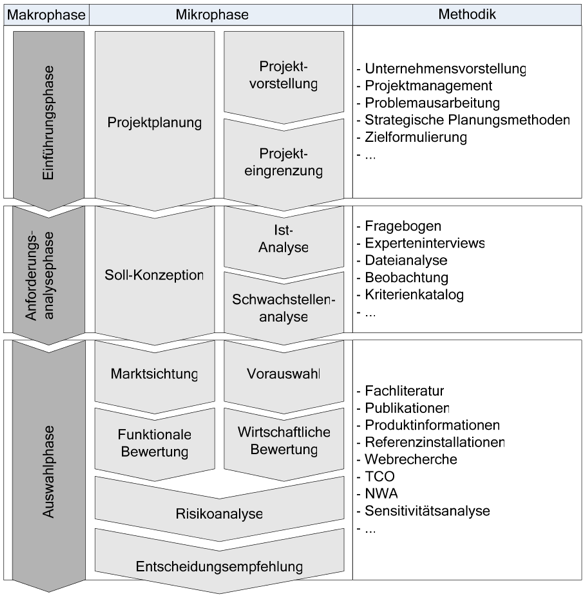
\includegraphics[width=10cm]{kapitel/gruppe4_1/bilder/vorgehensmodell_softwaremigration}
	\caption{Vorgehensmodell für Software-Migrationen nach \cite{migrationsleitfaden_2012}}
	\label{fig_vorgehensmodell_softwaremigration}	
\end{figure}

Das in Abbildung \ref{fig_vorgehensmodell_softwaremigration} ersichtliche Vorgehensmodell beschreibt die verschiedenen, notwendigen Phasen, die einer Migration vorausgehen. Die Genauigkeit dieser Planung ist hierbei maßgeblich für den späteren Erfolg der Migration. Im Rahmen dieser Ausarbeitung wurde beispielsweise die in der Abbildung ersichtliche Methodik des Experteninterviews angewandt, um Grundlagen für die Ist-Analyse zu erhalten.

In der Auswahlphase sind hierbei strategische, rechtliche und wirtschaftliche Aspekte zu berücksichtigen, ebenso wie der spätere Systembetrieb, die notwendigen organisatorischen Aspekte und Anforderungen an die Sicherheit der Systeme. Nach der Entscheidungsempfehlung werden dann eine oder mehrere Migrationsstrategien für die Einführung der neuen und die Ablösung der alten Software festgelegt.

\subsection{Migrationsstrategien}
Die Wahl der Migrationsstrategie ist jeweils fallbezogen zu prüfen. Es ist auch denkbar, für verschiedene Systeme verschiedene Strategien zu nutzen. Nachfolgend werden auszugweise durch Prof. Dr. Markus Nüttgens\footnote{\url{http://www.enzyklopaedie-der-wirtschaftsinformatik.de/wi-enzyklopaedie/lexikon/is-management/Integration-und-Migration-von-IT-Systemen/Ablosung-von-Altsystemen}} beschriebene Migrationsstrategien aufgeführt, welche in Abschnitt \ref{subsection_migrationsbeispiele} hinsichtlich der Verwendung durch die Migrationsbeispiele der Hochschule beleuchtet werden.

\begin{itemize}
	\item \textbf{Big Bang Approach (Cold Turkey Strategy):} Hierbei wird das Altsystem von Grund auf neu entwickelt und zu einem bestimmten Zeitpunkt zur Verfügung gestellt.	
	
	\item \textbf{Database First Approach / Database Last Approach:} Bei dieser Strategie wird erst das Datenbankmanagementsystem (Database First) migriert und anschließend alle Applikationen und Schnittstellen in ein neues System überführt. Database Last beschreibt hierbei den genau umgekehrten Vorgang.
	
	\item \textbf{Composite Database Approach:} Das neue Anwendungssystem wird schrittweise implementiert, während das Altsystem noch in Betrieb ist.
	
	\item \textbf{Chicken-Little Strategy:} Als Erweiterung des Composite Datebase Approach werden im Rahmen dieser Strategie zusätzliche Gateways entwickelt, welche für die Überführung der Daten aus dem Altsystem in das Zielsystem verantwortlich zeichnen.
	
	\item \textbf{Butterfly Methodology:} Hierbei geht es um eine reine Datenmigration, bei der eine Kooperation zwischen Alt- und Neusystem nicht notwendig ist.  Die Entwicklung des neuen Systems wird also von der Migration der Daten separiert.
\end{itemize}


\subsection{Migrationsbeispiele}
\label{subsection_migrationsbeispiele}

Die Hochschule Emden/Leer nutzt derzeit für Ihren Internetauftritt das Enterprise Content Management System TYPO3 in der Version 4.5. Die Dokumentenverwaltungssoftware Alfresco wird derzeit noch nicht genutzt. 

Die folgenden Beispiele behandeln eine mögliche Migration von TYPO3 auf eine aktuelle Version inkl. Erstellung eines responsive Designs, sowie die Neueinführung von Alfresco. Da die aktuelle Version von Alfresco auch die Möglichkeit bietet Web Content zu verwalten, wäre theoretisch auch eine Migration des derzeitigen Internetauftritts in ein neu eingeführtes Alfresco-System denkbar.

\subsubsection{Responsive Website mit TYPO3}
TYPO3\footnote{\url{http://typo3.org/typo3-cms/overview/}, abgerufen am 28.05.2015} ist ein Open Source Enterprise Content Management System zur Verwaltung webbasierter Inhalte. Es ist multilingual, hoch skalierbar und bietet ein aktives Sicherheitsmanagement.

\paragraph{Ist-Zustand}
Die Hochschule Emden/Leer nutzt derzeit ein TYPO3-Sytem in der Version 4.5 LTS (Long Term Support). Das System ist derzeit noch nicht für die Anforderungen mobiler Endgeräte (responsive Design) gerüstet. Es werden verschiedene Extensions von TYPO3 genutzt, möglicherweise auch eigens für die Hochschule entwickelte Extensions. Mitarbeiter und Studenten sind als Benutzer innerhalb des CMS angelegt und können sich in einen geschützten Bereich über die Extension FE-Login anmelden.

Für die derzeit eingesetzte Version von TYPO3 gibt es keinen Support mehr, so dass – weder für den TYPO3-Kern, noch für die Extensions – neue Sicherheitspatches zur Verfügung gestellt werden. Dies stellt ein Sicherheitsrisiko für die Hochschule dar. Allein aus diesem Grund sollte eine Migration auf ein aktuelles System erwogen werden. Ferner nutzt ein Großteil der Besucher mobile Endgeräte, die aktuell nicht unterstützt werden.

\paragraph{Soll-Zustand}\mbox{}\\
Das neue System soll über folgende Merkmale verfügen:
\begin{itemize}
\item lange Support-Zeit, damit Sicherheitspatches eingespielt werden können
\item Unterstützung von mobilen Endgeräten
\item Übernahme bestehender Extensions oder Vorhandensein von Alternativen hierzu
\item Barrierefreiheit, damit auch Benutzer mit Handicap den Internetauftritt besuchen können
\item Suchmaschinenoptimierung (SEO)
\item Anbindung an die Benutzerverwaltung (Single-Sign-On) der Hochschule (bereits realisiert)
\end{itemize}
Hierzu wird zunächst ein strategisch günstiger Migrationsplan erstellt.

\paragraph{Migrationsplan}\mbox{}\\
Um einen möglichst langen Supportzeitraum zu gewährleisten ist die Verwendung einer LTS-Version (Long Term Support) anzuraten. Die derzeit aktuelle Version ist 6.2.12 LTS (Stand 27.05.2015), welche noch bis Ende März 2017 supportet wird.

Derzeit ist bereits die Version 7.2.0 verfügbar, allerdings noch nicht als LTS-Version. Diese ist für Herbst 2015 avisiert. 

Da die Migration einige Zeit in Anspruch nehmen wird, ist es sinnvoll, direkt auf die Version 7.x LTS zu migrieren, da diese dann verfügbar sein wird. Hierfür sind allerdings Zwischenschritte vorzusehen, da eine direkte Migration von Version 4.5 auf 7.x nicht möglich ist.\footnote{\url{http://wiki.typo3.org/Upgrade}, abgerufen am 28.05.2015} Es muss zunächst eine Migration auf die Version 6.2 LTS und von dort auf die Version 7.x erfolgen. Nachfolgend wird somit von einer Migration auf die Version 7.x LTS ausgegangen.

Vor der Migration ist eine Überprüfung aller derzeit genutzten Extensions erforderlich. Dabei muss geprüft werden, ob diese in der neuen Version noch gültig und lauffähig sind. Ist dies nicht der Fall, müssen Alternativen gesucht werden und deren Realisierung in die Planung einfließen. Insbesondere selbst geschriebene Extensions müssen hinsichtlich der Lauffähigkeit überprüft und ggf. ein Konzept zur Anpassung erstellt werden.

\subparagraph{Hardwareanforderungen}\mbox{}\\
Für eine erfolgreiche Migration sind bestimmte Hardwareanforderungen Voraussetzung. Unter anderem muss mindestens PHP 5.5, MySQL 5.5 und mehr als 200 MB freier Plattenplatz zur Verfügung stehen. Die genauen Konfigurationseinstellungen inkl. allen benötigten Module sind den Installationsvorgaben der TYPO3 Association zu entnehmen.

\subparagraph{Entwicklungssystem}\mbox{}\\
Zur Realisierung des neuen Systems wird ein Entwicklungssystem mit den oben beschriebenen Hardwareanforderungen aufgesetzt. Über einen Dump der Datenbank werden die Daten des Produkivsystems in die Datenbank des Entwicklungssystems übertragen. Das gesamte Dateisystem des TYPO3-Produktivsystems wird ebenfalls auf das Entwicklungssystem übertragen. Dort werden dann die Konfigurationseinstellungen von TYPO3 angepasst, damit ein identisches, lauffähiges System entsteht.

Innerhalb dieses Systems erfolgt die Migration auf die verschiedenen Versionen, die Anpassung der Extensions und die im Rahmen der Migration notwendige Softwareentwicklung.

\subparagraph{Migration}\mbox{}\\
Im Rahmen der Migration müssen Softwaretechnisch folgende Punkte berücksichtigt werden:
\begin{itemize}
\item Migration des TYPO3-Kerns
\item Migration aller eingesetzten Extensions
\item Anpassung selbstgeschriebener Extensions
\item Umstellung des Layout-Konzeptes von TYPO3 (von derzeit wahrscheinlich Templa-Voilà) auf Fluid-Templating
\item Schaffung einer Basis für responsive Design, beispielsweise auf Basis des Frameworks Bootstrap
\item Erweiterung / Anpassung der TypoScript-Programmierung
\item Anpassung Menüprogrammierung (TypoScript und Template)
\item Neuerstellung benötigter Fluid-Templates auf Basis von Haupttemplates und Partials
\item Programmierung eigener Extensions, falls notwendig
\end{itemize}

\subparagraph{Produktivsetzung}\mbox{}\\
Die Ablösung des derzeitigen Systems erfolgt anhand der Migrationsstrategie Big Bang Approach, da mit dem Entwicklungssystem ein fertig entwickeltes und hinsichtlich des Datenbestandes aktuelles System zur Verfügung steht. Die Produktivsetzung erfolgt in umgekehrter Reihenfolge wie die Einrichtung des Entwicklungssystems, also mit Datenbank-Dump, Datei-Migration und ggf. TYPO3-Konfigurations-anpassungen. Hierdurch ist die Downtime für den Internetauftritt der Hochschule Emden minimal.

\subsubsection{Alfresco}
Alfresco\footnote{\url{https://www.alfresco.com/de/solutions/document-management}, abgerufen am 28.05.2015} ist ein Dokumenten-Management-System welches als Open-Source-Plattform offene Standards unterstützt. Hiermit lässt sich der gesamte Content auf einer einzelnen Plattform konsolidieren und damit die Benutzerfreundlichkeit erhöhen und die Kosten senken.

Luis Cabaceira\footnote{\url{http://de.slideshare.net/LuisCabaceira/sizing-your-alfrescoplatform}, abgerufen am 27.05.2015} hat die nachfolgende Grafik erstellt, die eine Übersicht über die Funktionen von Alfresco gibt:

\begin{figure}[h!]
	\centering
	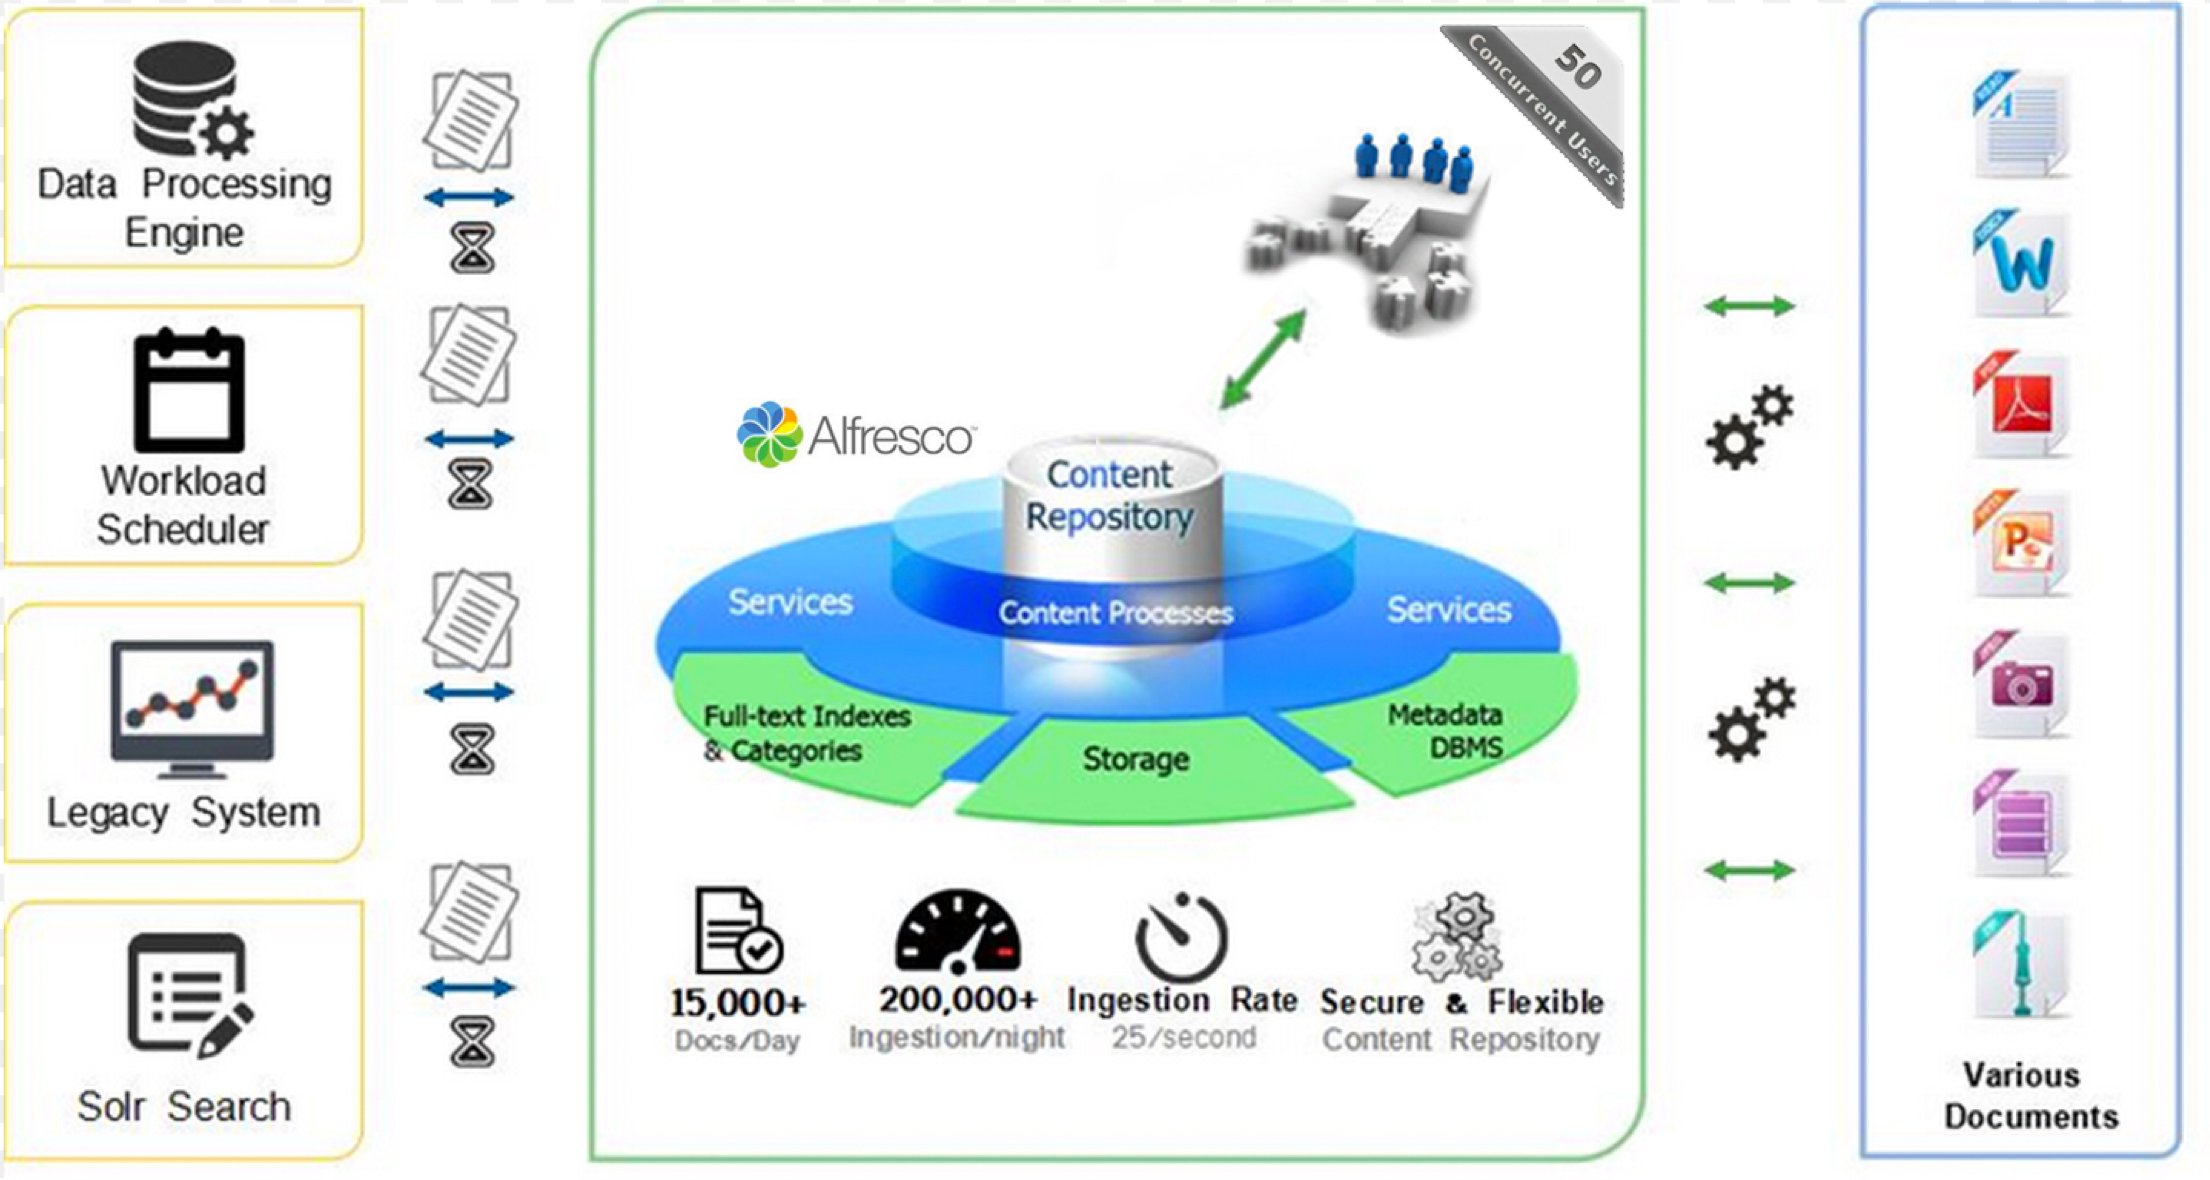
\includegraphics[width=10cm]{kapitel/gruppe4_1/bilder/uebersicht_alfresco}
	\caption{Übersicht Alfresco nach Luis Cabaceira}
	\label{fig_uebersicht_alfresco}
\end{figure}

Peter Franke – Leiter des Rechenzentrums der Hochschule Braunschweig/Wolfenbüttel – berichtet von positiven Erfahrungen seit der Einführung von Alfresco.\footnote{\url{http://www.ostfalia.de/export/sites/default/de/rz/documents/it-konzept-2011.pdf}, abgerufen am 27.05.2015}

\paragraph{Ist-Zustand}
\paragraph{Soll-Zustand}
\paragraph{Migrationsplan}





\section{Zuständigkeiten (TiK)}
\label{section_zustaendigkeiten}
In diesem Kapitel wird auf die Zuständigkeiten in Bezug auf die Informationsbereitstellung an der Hochschule Emden/Leer näher eingegangen. Es wird dargestellt, welche Bereiche bereits zentral an der Informationsbereitstellung beteiligt sind. Ebenso wird auf die Besonderheiten einzelner Fachbereiche, zentraler Einrichtungen und dem Präsidium detaillierter eingegangen (siehe Abbildung \ref{fig_organigramm_HS}). 

\begin{figure}[h!]
	\centering
	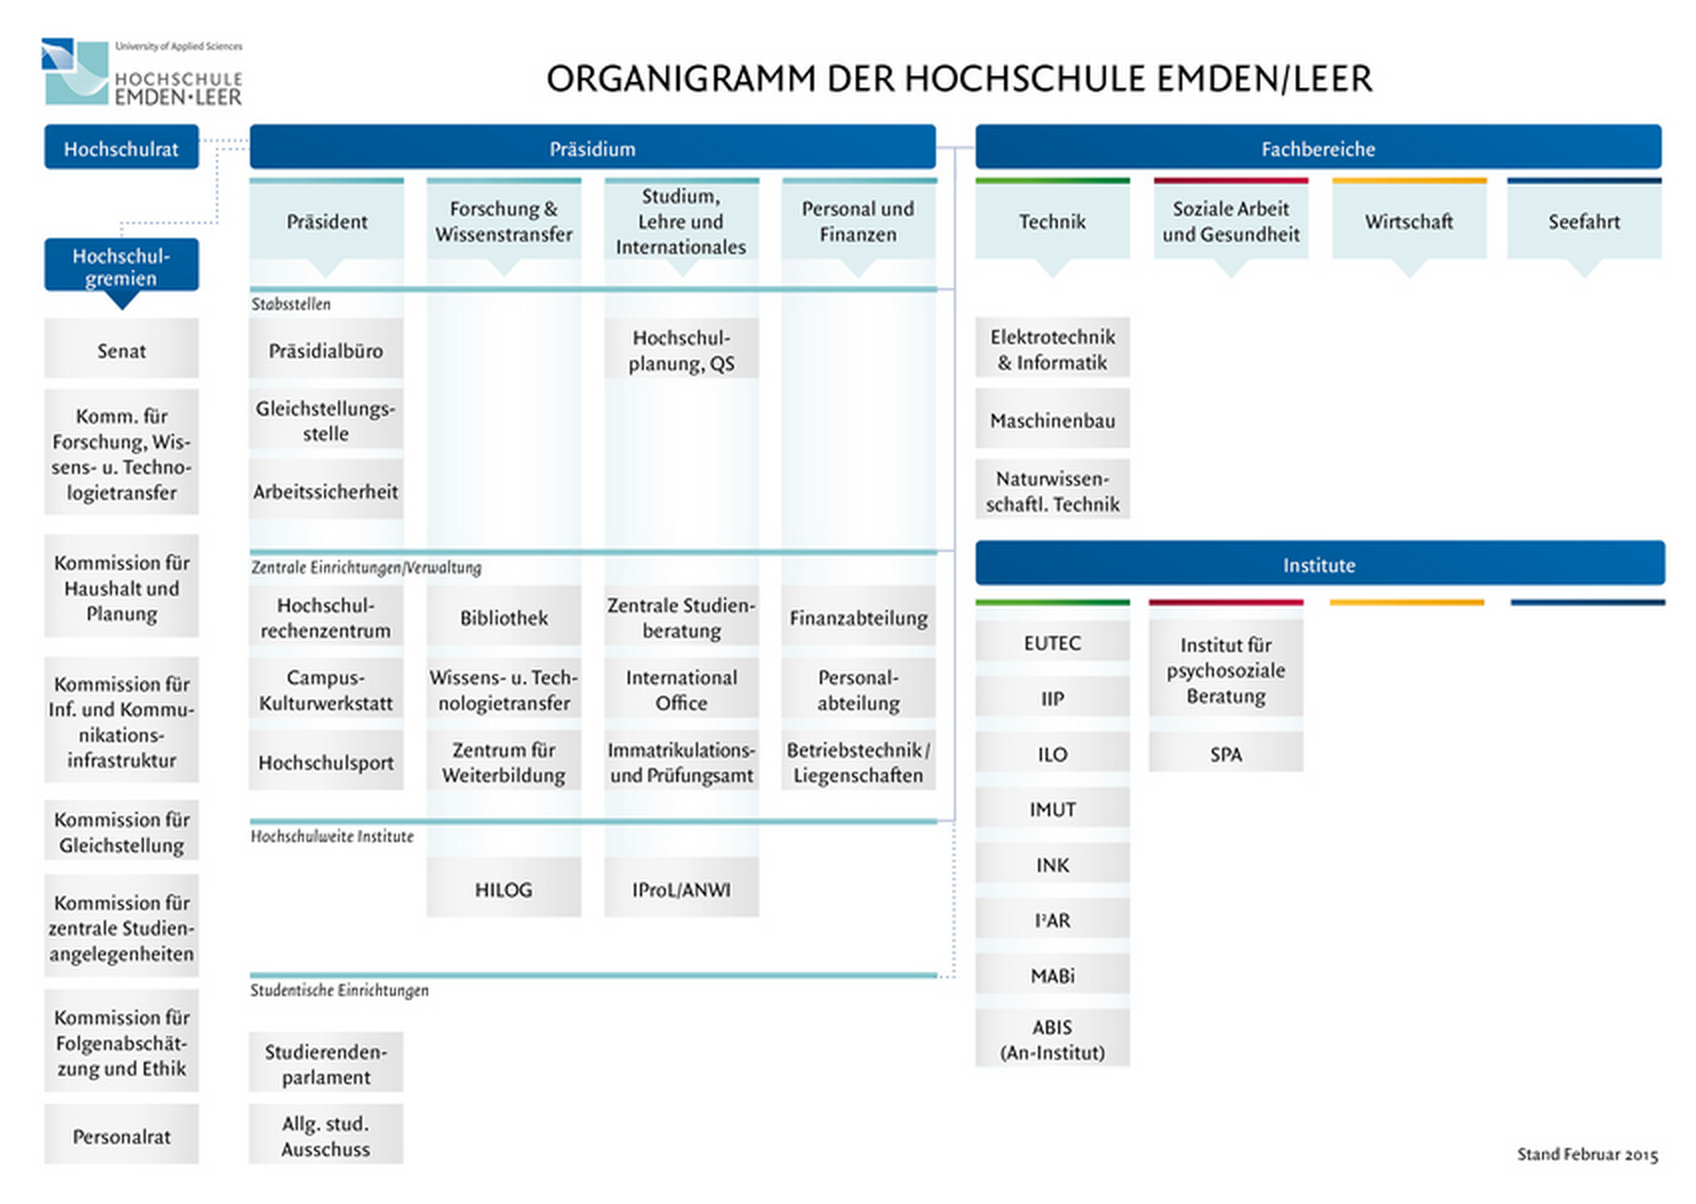
\includegraphics[width=14cm]{kapitel/gruppe2/bilder/organigramm_HS}
	\caption{Organigramm der Hochschule Emden/Leer}
	\label{fig_organigramm_HS}
\end{figure}

Nachfolgend wird ein Überblick über die IT-Systeme gegeben, welche sowohl von Mitarbeitern als auch Studierenden verwendet werden (siehe Abbildung  \ref{fig_zentrale_systeme}). Bei allen zentralen Systemen ist bereits eine Authentifizierung über Single Sign On (SSO) gegeben (siehe Kapitel \ref{realisierung_der_serviceorientierung} auf Seite \pageref{realisierung_der_serviceorientierung}).

\begin{figure}[h!]
	\centering
	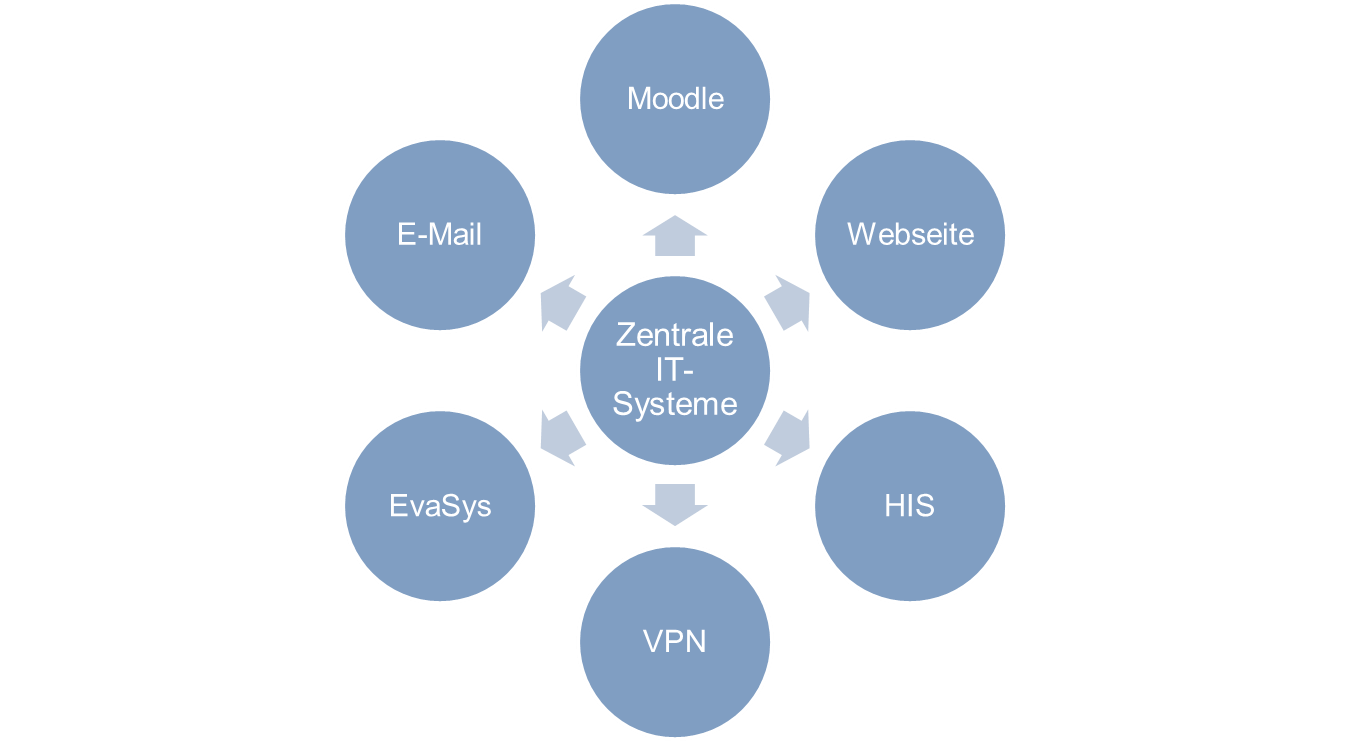
\includegraphics[width=14cm]{kapitel/gruppe2/bilder/zentrale_systeme}
	\caption{Zentrale Systeme für Mitarbeiter und Studenten}
	\label{fig_zentrale_systeme}
\end{figure}


\subsection{Fachbereiche}
Die einzelnen Fachbereiche sind unter anderem durch die Mitgliedschaft in Arbeitsgruppen in den Informationsbeschaffungsprozess involviert.

Alle Fachbereiche verfügen über die Berechtigung, relevante Informationen im Infosys darzustellen. Beim InfoSys handelt es sich um eine zentrale Plattform zur Darstellung von organisatorischen Informationen. Diese können direkt online auf der öffentlichen Webseite der Hochschule Emden/Leer eingesehen werden oder in den Eingangsbereichen der jeweiligen Fachbereiche vor Ort über entsprechende Monitore. Es werden, nach Fachbereich sortiert, die wichtigsten Neuigkeiten als Newsticker dargestellt und der Zugriff auf alle Vorlesungspläne der Fachbereiche ist gegeben, um so zügig auf organisatorische Inhalte zugreifen zu können (siehe Abbildung \ref{fig_InfoSys}). Aufbauend auf dem InfoSys wird eine selbst entwickelte Android App zur Verfügung gestellt.

\begin{figure}[h!]
	\centering
	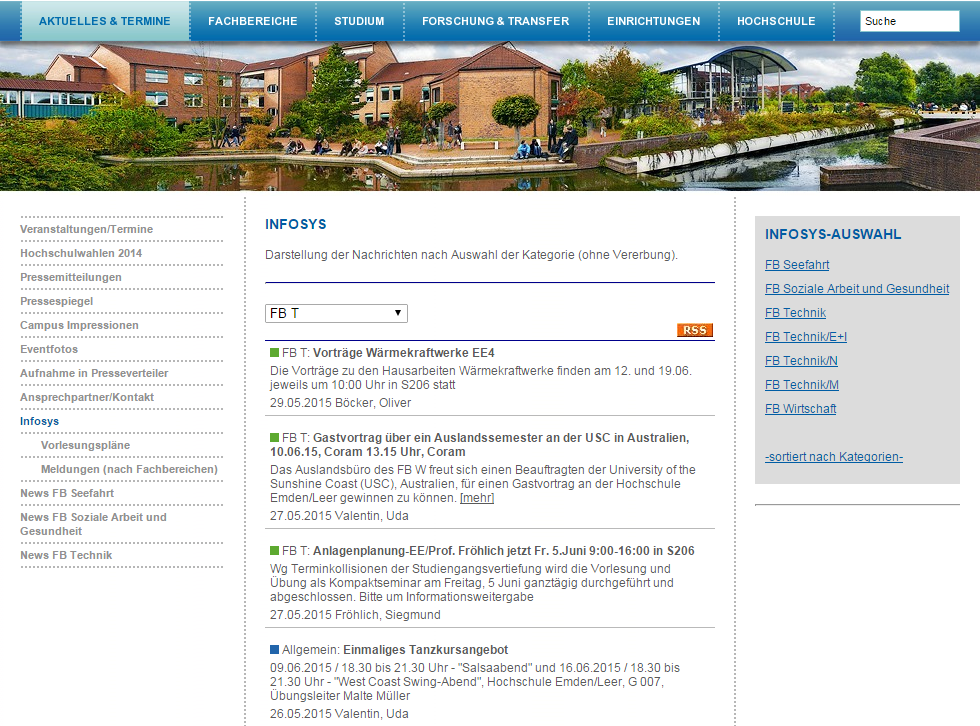
\includegraphics[width=14cm]{kapitel/gruppe2/bilder/InfoSys}
	\caption{Exemplarischer Screenshot des INFOSYS des Fachbereiches Technik}
	\label{fig_InfoSys}
\end{figure}

In den nachfolgenden Kapiteln wird auf die Besonderheiten der einzelnen Fachbereiche eingegangen.

\subsubsection{Seefahrt}
Bei dem Fachbereich Seefahrt handelt es sich um einen relativ kleinen Fachbereich. Seefahrt ist  nur am Standort Leer vertreten. Dieser Fachbereich verwendet kein zentrales System zur Vorlesung und Raumplanung, sondern eine Eigenentwicklung.

\subsubsection{Technik}
Eine Besonderheit dieses Fachbereiches ist es, dass für den Laborbetrieb ein Netzwerk neben dem zentralen Netzwerk der Hochschule Emden/Leer betrieben wird. Da unter anderem der Bereich „IT-Sicherheit“ ein wichtiger Aspekt in dem Studiengang Informatik ist, kommt es zu besonderen Konstellationen im Bereich der Forschung. Dieser Bereich verwaltet sein Netz selbst und ist somit autark vom allgemeinen Hochschulrechennetz. Es besteht jedoch eine enge Zusammenarbeit zwischen dem Bereich Technik (im speziellen E+I) und dem Rechenzentrum, so dass unter anderem gegenseitige Zugriffsrechte bestehen. 

\subsection{Präsidium}
\label{praesidium_label}

Die Hochschule Emden/Leer setzt Moodle als Lernplattform ein (siehe Abbildung 
Das Präsidium, insbesondere mit dem Bereich zentrale Verwaltung, ist über  Arbeitsgruppen in den Informationsbeschaffungsprozess involviert. Zudem verfügt das Präsidium mit einer Stabsstelle über einen zentralen Bereich im Bezug auf die Repräsentation von Informationen.  Das Präsidialbüro ist unter anderem für den Bereich Hochschulmarketing zuständig. Auch ist in der Stabstelle des Präsidialbüros die Presse- und Öffentlichkeitsarbeit angesiedelt.

\subsection{Zentrale Verwaltung}
Die zentrale Verwaltung verwendet im Bereich Personalverwaltung und Finanzen ausschließlich „SAP“ als Buchhaltungssystem. Zur Organisation von Lehr- und Vorlesungsplanung wird das System UNTIS Plus verwendet. Ebenso wird für die Urlaubsplanung, Zeiterfassung und das Gebäudeschließsystem ein eigenständiges System verwendet. Speziell für die Aufbereitung von Kennzahlen und Zahlen wird eine Eigenentwicklung als BIS (Business Intelligence System) verwendet. 

\subsubsection{Rechenzentrum}
Das Hochschulrechenzentrum der Hochschule ist stark in die Administration und Pflege der bestehenden Systeme zur Informationsbereitstellung involviert. Neben der Administration von bestehenden Systemen obliegt dem Hochschulrechenzentrum ebenfalls der Endkundensupport.

\subsection{Arbeitsgruppen zum Informationsaustausch und zur Informationsbereitstellung}
\label{subsection_arbeitsgruppen_informationsaustausch}
Die Zuständigkeiten an der Hochschule, in Bezug auf Informationssammlung, Beschaffung und Aufbereitung von Informationen, ist bereits durch Arbeitsgruppen in wichtigen Bereichen geregelt. Durch das Interview mit dem Leiter des Hochschulrechenzentrums konnte ein Einblick in die bestehenden Gremien geschaffen werden. Diese treffen sich regelmäßig zum Informations-, Wissens- und Erfahrungsaustausch.

Es existieren drei Arbeitsgruppen, welche für die Informationsverteilung in den jeweiligen Bereichen relevant sind:

\begin{itemize}
	\item Zahlen, Daten und Fakten (ZDF)
	\item WEB
	\item Moodle
\end{itemize}

\subsubsection{Zahlen, Daten und Fakten (ZDF)}
ZDF setzt sich zusammen aus den Verwaltungsabteilungen Finanzen, Personal, Presse und Rechenzentrum. Dieses Gremium ist zuständig für die Erstellung und Aufbereitung von Kennzahlen. Dies können zum Beispiel aktuelle Kennzahlen zu eingeschriebenen Studierenden pro Studiengang sein.  ZDF ist für einen Unterbereich der offiziellen Webseite der Hochschule zuständig. Die Kennzahlen und Zahlen werden gruppenbasiert erstellt. Je nach Berechtigung werden Kennzahlen in unterschiedlichen Detailgraden dargestellt. So erhalten Dekane mehr Informationen als Mitarbeiter. Öffentlich zugänglich sind nur generische Kennzahlen. 

\subsubsection{WEB}
Es existiert eine Arbeitsgruppe, welche für die Gestaltung und den Inhalt der öffentlichen Webseite der Hochschule verantwortlich ist. In dieser Arbeitsgruppe sind aus jedem Fachbereich Repräsentanten mit einbezogen. Die Leitung des Web-Teams obliegt dem Präsidialbüro.\footnote{\url{http://www.hs-emden-leer.de/fileadmin/user_upload/Einrichtungen/Praesidialbuero/Organigramm_Praesidialbuero_Juli2013_01.pdf}}

\subsubsection{Moodle}
In der Arbeitsgruppe „Moodle“ sind sowohl Repräsentanten aus jedem Fachbereich involviert sowie auch Repräsentanten aus der Verwaltungsebene. Da das Moodle E-Learning System mittlerweile als ein zentrales Moodle für alle Bereiche eingeführt wurde, haben die Mitglieder aus den Fachbereichen unter anderem das Recht, Kurse im Moodle freischalten zu können. Auf die E-Learning Plattform „Moodle“ wird detaillierter im Kapitel \ref{paragraph_moodle} auf Seite \pageref{paragraph_moodle} eingegangen.

\section{Abwägung des Einsatzes eines Informationsmanagements an der Hochschule Emden Leer}
Das Soll-Konzept analysiert die Ist-Situation um festzustellen, ob es generell einer Verbesserung des Informationsmanagements bedarf und wo diese anzusetzen sind oder ob noch kein Informationsmanagement besteht und aufgebaut werden muss. Dazu sind verschiedene Aspekte zu beleuchten. Neben der Anforderung des Marketings und neben den  technischen Neuerungen und Umsetzungen ist zu klären, wer die strategische und operative Führung übernehmen soll. 

Im klassischen Informationsmanagement ist dies die Aufgabe eines Chief Information Officers. Der Informationsmanager dient dabei als zentrale Schnittstelle zwischen technischen, organisatorischen und wirtschaftlichen Teilbereichen und dient dort als sogenannter Mittler und untersucht dafür die Informations- und Kommunikationstechniken in allen unterschiedlichen Bereichen um diese sinnvoll einzusetzen.\footnote{\cite[86]{krcmar_einfuhrung_2015}}

\begin{figure}[h!]
	\centering
	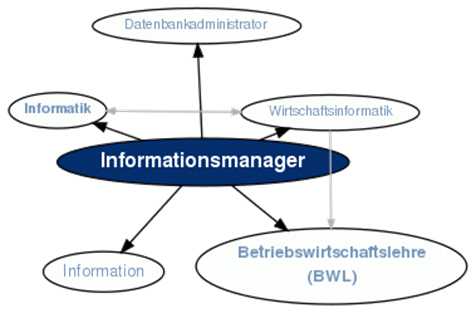
\includegraphics[width=10cm]{kapitel/gruppe3/bilder/definition_informationsmanager}
	\caption{Definition Informationsmanager}
	\label{fig_definition_informationsmanager}
\end{figure}

\subsection{Analyse des Ist-Zustandes}
Bezug nehmend auf die Abbildung \ref{fig_organigramm_HS} und der festgestellten Ist-Analyse ist festzuhalten, dass der Hochschule Emden kein Informationsmanagement im klassischen Sinne zugrunde liegt, sondern ein zentrales Informationssystem.

Es werden verschiedene Dienste und Möglichkeiten wie Moodle, Eduroam zur Verfügung gestellt und in Anspruch genommen.

Es gibt keine Verwaltung, sondern verschiedene Bereiche, die unterteilt sind in Arbeitsgruppen, Abteilungen sowie Rechenstelle und Pressestelle.

Weiterhin beinhaltet das Informationssystem verschiedene Prozesse zum Datenaustausch, bzw. Datenfluss und Backuptransfer  aus verschiedenen Systemen.\footnote{Ist-Situation \#8}

Die Nutzung des gegenwärtigen Informationssystems wird unterschiedlich stark genutzt oder ausgelastet.

Von den zentralen Einrichtungen nehmen das Hochschulrechenzentrum und die Bibliothek einen wichtigen Platz in der Hochschule ein. Das Hochschulrechenzentrum übernimmt derweil viele Aufgaben der Informationsverwaltung und Planung.

Doch nicht nur da werden Informationen gesammelt und  ausgewertet. Die Hochschule in Emden definiert eine ganze Reihe von Arbeitsgruppen, beispielsweise die Arbeitsgruppe Zahlen, Daten, Fakten, die Kennzahlen der Hochschule und der einzelnen Fachbereiche sammelt und diese auswertet.\footnote{Ist-Situation \#8}

Aktuell besteht keine Vernetzung verschiedener Intranetzsysteme zwischen verschiedenen Hochschulen.

\subsection{Analyse des zu erwartenden Soll-Zustandes}
Nach Betrachtung der Best-Practice Beispiele anderer Hochschulen, lässt sich erkennen, dass jede Hochschule und auch Universität den Umgang des Informationsmanagements anders angeht. So spielen verschiedene Faktoren eine Rolle, die an jeder Hochschule unterschiedlich ausgelegt sind.

Ein Vergleich der betrachteten Hochschulen mit der Hochschule Emden zeigt, dass Emden eine wesentlich kleinere Hochschule ist und somit andere Ansprüche sowie nicht so komplexe Strukturen besitzt, als beispielsweise die WWW Münster, die über 40.000 Studierende pflegt.

Trotz unterschiedlich integrierter Möglichkeiten zur Umsetzung des jeweiligen Informationsmanagements, gibt es doch Bereiche die gleich oder relativ ähnlich sind. So sind Bibliotheken, Gremien, Ausschüsse, ebenso wie Fachbereiche und auch das Präsidium Teil einer jeden Hochschule oder Universität.

Es ist zu schauen wo sich das Informationsmanagement ansetzen lässt um mehrere Bereiche und Bestandteile untereinander zu verbinden. Fakt ist, dass es in Emden bereits Arbeitsgruppen gibt, die bestimmte Informationen gewinnen und filtern. So wäre der Aufbau einer neuen Struktur eine Möglichkeit zur Verbesserung des Informationsaustausches.

\subsection{Soll-Möglichkeit}
\subsection{Zu erwartende Kosten}
\subsection{Prognose und zu erwartender Verlauf / Fazit}


\chapter{Kosten- und Zeitplanung}
	\chapter{Zusammenfassung}
	\printbibliography[heading=bibintoc, title=Literatur- und Quellenverzeichnis]
%\addcontentsline{toc}{chapter}{Listings}
\listoftables
\listoffigures
%\lstlistoflistings
	\appendix
\end{document}